\documentclass[12pt, a4 paper]{article}
% Set target color model to RGB
\usepackage[inner=2.5cm,outer=2.5cm,top=3cm,bottom=3cm]{geometry}
\usepackage{latexsym}           % math symbols that were omitted in latex2e
\usepackage{amsbsy}             % bold greek defs
\usepackage{amsmath,graphicx}
\usepackage{bbm}
\usepackage{mathrsfs}
\usepackage{stmaryrd}
\usepackage{graphics}
\usepackage{acronym}
\usepackage{longtable}
\usepackage{mathtools}
\usepackage{setspace}
\usepackage{cite}
\usepackage{array}
\usepackage{amsmath,amsthm}
\usepackage{amssymb}
\usepackage{wasysym,url}
\usepackage{fixltx2e,amsmath}
\usepackage{setspace,float}
\usepackage{color}
\usepackage{cases,bm}
\usepackage{mathrsfs}
\usepackage{enumitem}
\usepackage{hyperref}
\usepackage{mathtools,cuted}
\usepackage[linesnumbered,ruled,vlined]{algorithm2e}
\usepackage{epsfig}
\usepackage{color}
\usepackage{sectsty}
\usepackage{subfigure}
\DontPrintSemicolon
\hypersetup{%
pdfauthor={Abijith J Kamath},%
pdftitle={Homework},%
pdfkeywords={Tikz,latex,bootstrap,uncertaintes},%
pdfcreator={PDFLaTeX},%
pdfproducer={PDFLaTeX},%
}

\newcommand{\ra}[1]{\renewcommand{\arraystretch}{#1}}

\newtheorem{thm}{Theorem}[section]
\newtheorem{prop}[thm]{Proposition}
\newtheorem{lem}[thm]{Lemma}
\newtheorem{cor}[thm]{Corollary}
\newtheorem{defn}[thm]{Definition}
\newtheorem{rem}[thm]{Remark}
\numberwithin{equation}{section}

\newcommand{\homework}[6]{
   \pagestyle{myheadings}
   \thispagestyle{plain}
   \newpage
   \setcounter{page}{1}
   \noindent
   \begin{center}
   \framebox{
      \vbox{\vspace{2mm}
    \hbox to 6.28in { {\bf E1 213:~Pattern Recognition and Neural Networks\hfill {\small Spring 2021}} }
       \vspace{6mm}
       \hbox to 6.28in { {\bfseries \Large \hfill #1  \hfill} }
       \vspace{6mm}
       \hbox to 6.28in { {\it Author: {\rm Abijith J. Kamath}} \hfill {\small {\it Email:} abijithj@iisc.ac.in}}
      \vspace{2mm}}
   }
   \end{center}
   \markboth{E1 213 -- #1}{E1 213 -- #1}
   \vspace*{4mm}
}

\newcommand{\problem}[1]{~\\\fbox{\textbf{#1}}\newline\newline}
\newcommand{\subproblem}[1]{~\newline\textbf{(#1)}}

\newcommand{\solution}{~\newline\textbf{\textit{(Solution)}} }

\linespread{1.3}

\setlength{\intextsep}{20pt} % Vertical space above & below [h] floats
\setlength{\textfloatsep}{20pt} % Vertical space below (above) [t] ([b]) floats
\setlength{\abovecaptionskip}{10pt}
\setlength{\belowcaptionskip}{10pt}

\newcommand{\by}{\mathbf{y}}
\newcommand{\bx}{\mathbf{x}}
\newcommand{\bX}{\mathbf{X}}
\newcommand{\bW}{\mathbf{W}}
\newcommand{\bA}{\mathbf{A}}
\newcommand{\bF}{\mathbf{F}}
\newcommand{\rr}{\mathbb{R}}
\newcommand{\cc}{\mathbb{C}}
\newcommand{\Ex}{\mathbb{E}}
\newcommand{\TT}{\mathsf{T}}
\newcommand{\HH}{\mathsf{H}}

\newcommand{\bmu}{\boldsymbol{\mu}}
\newcommand{\btheta}{\boldsymbol{\theta}}
\newcommand{\bSigma}{\boldsymbol{\Sigma}}

\chapterfont{\fontfamily{lmss}\selectfont}
\sectionfont{\fontfamily{lmss}\selectfont}
\subsectionfont{\fontfamily{lmss}\selectfont}

\begin{document}
\homework{Assignment 2: Linear Models}{}





\section{Introduction}
\label{sec:intro}

Let patterns be in $\rr^{d}$ and consider the $2$-class classification problem - given a pattern $\bx$, classify the pattern with a label $y$. In classification using linear least-squares and logistic regression the training data $\{\bx^{(i)}, y^{(i)}\}_{i=1}^{n}$ is used to directly learn a discriminative function that scores the new patterns, and the classification is achieved by thresholding the score.

% ------------------------------------------------------------------------------------------------------------------------------------------------------

\subsection{Linear Least-Squares Classification}
\label{subsec:linearRegression}

Consider the two-class classification problem of classifying patterns into labels $y \in \{-1, +1\}$. The discriminative function in linear least-squares classification is a function that is linear in the weights, using features of the patterns. In this case, the patterns are directly used as the features, and the discriminative function is given as:
\begin{equation}
	f(\bx) = \sum_{i=1}^{d} w_{i} x_{i} + w_{0} = \bW^{\TT} \tilde{\bx},
\label{eq:linearDiscriminator}
\end{equation}
where $\bW = [w_{0}, w_{1}, \cdots, w_{d}] \in \rr^{d+1}$ are the weights to be learnt from the training samples and $\tilde{\bx}$ is the augmented feature vector with $1$ padded as its first entry. The classification is then done using the sign of the score function $f(\bx)$. \\

This can be easily extended to a multi-class classifier by consider similar score functions for each class. The labels are converted to one-hot vectors. The decision rule is to choose the class that gives the largest score. \\

The weights are obtained by minimising the $\ell^{2}$-norm between the predictions $f(\bx^{i})$ and $y^{(i)}$:
\begin{equation}
	J(\bW) = \frac{1}{2} \sum_{i=1}^{n} \left( \bW^{\TT}\bx^{(i)} - y^{(i)} \right)^{2}.
\label{eq:lsClassifier}
\end{equation}
The minimiser of $J(\bW)$ can be obtained in closed form as $\bW^{*} = \bA^{\dagger} \by$, where $\bA = [\bx^{(1)} \; \bx^{(2)} \; \cdots ; \bx^{(n)}]^{\TT}$ and $\by = [y^{(1)} \; y^{(2)} \; \cdots \; y^{(n)}]^{\TT}$. This directly extends to the multi-class classifier with the labels in $\by$ taken to be one-hot vectors. The closed form solution will then give the complete weight matrix.

% ------------------------------------------------------------------------------------------------------------------------------------------------------

\subsection{Logistic Regression}
\label{subsec:logisticRegression}

Consider the two-class classification problem of classifying patterns into labels $y \in \{-1, +1\}$. The discriminative function in logistic regression is the sigmoid:
\begin{equation}
	f(\bx) = \frac{1}{1+e^{-\bW^{\TT}\tilde{\bx}}},
\label{eq:logisticDiscriminator}
\end{equation}
which is treated as the probability of assigning $y=+1$ to the pattern $\bx$ ($\bW$ and $\tilde{\bx}$ have the same meaning as above). If the score is less than $1/2$, the pattern is classified into $y=-1$. \\

The weights are obtained from the training samples by maximising the likelihood using gradient descent. The weights cannot be obtained in closed form like in Linear Least-Squares classification. The gradient descent updates for the weights is given by:
\begin{equation}
	\bW^{+} = \bW + \eta \sum_{i=1}^{n} \left( y^{(i)} - \sigma(\bW^{\TT}\tilde{\bx}^{(i)}) \right) \tilde{\bx}^{(i)},
\label{eq:logGD}
\end{equation}
where $\sigma$ is the sigmoid function and $\eta$ is the step size. \\

Logistic regression can be extended to multi-class classification by taking the score function for each class to be the softmax function, which is interpreted as assigning the probability of the pattern being in each class and then choosing the class that gives the highest probability.

% ------------------------------------------------------------------------------------------------------------------------------------------------------

\section{Linear Classification on Synthetic Data}
\label{sec:LRandLOG}

\problem{Problem (1.a) Gamma-distributed Classes in 2D}
\label{prob:1.a}

Let the class conditionals be modelled as Gamma distributions with different shape and scale parameters. The $2$-class linear least-squares (LS) classifier is trained by minimising (\ref{eq:lsClassifier}) and logistic regression (LOG) is trained using gradient descent with constant step-size using (\ref{eq:logGD}). \\

{\it \bfseries Results:} Figure \ref{fig:LS_LOG_Gamma} shows the accuracies of classification in confusion matrices and the samples along with the discriminant function. The first and third columns shows the confusion matrices of the linear classifier and logistic regression, respectively with varying training sizes. The second and fourth column shows the samples along with the discriminant function. The accuracies reported are averaged over $10000$ realisations and one of the discriminant functions is plotted. \\

\begin{figure}
\centering
\subfigure[LS, Size $10$]{\label{fig:a}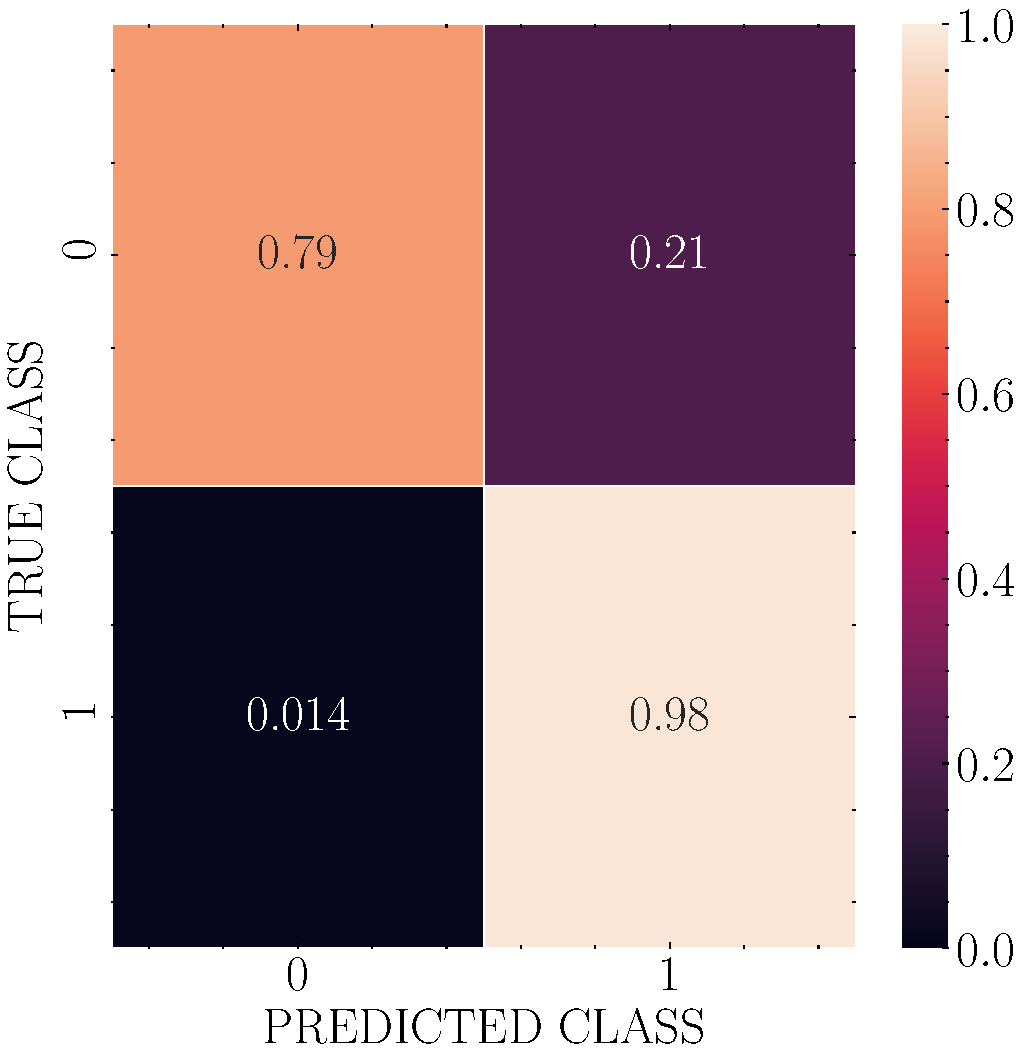
\includegraphics[width=1.5in]{../results/ex1/acc_LS_dataset_Gamma_size_10}}
\subfigure[LS Classifier]{\label{fig:a}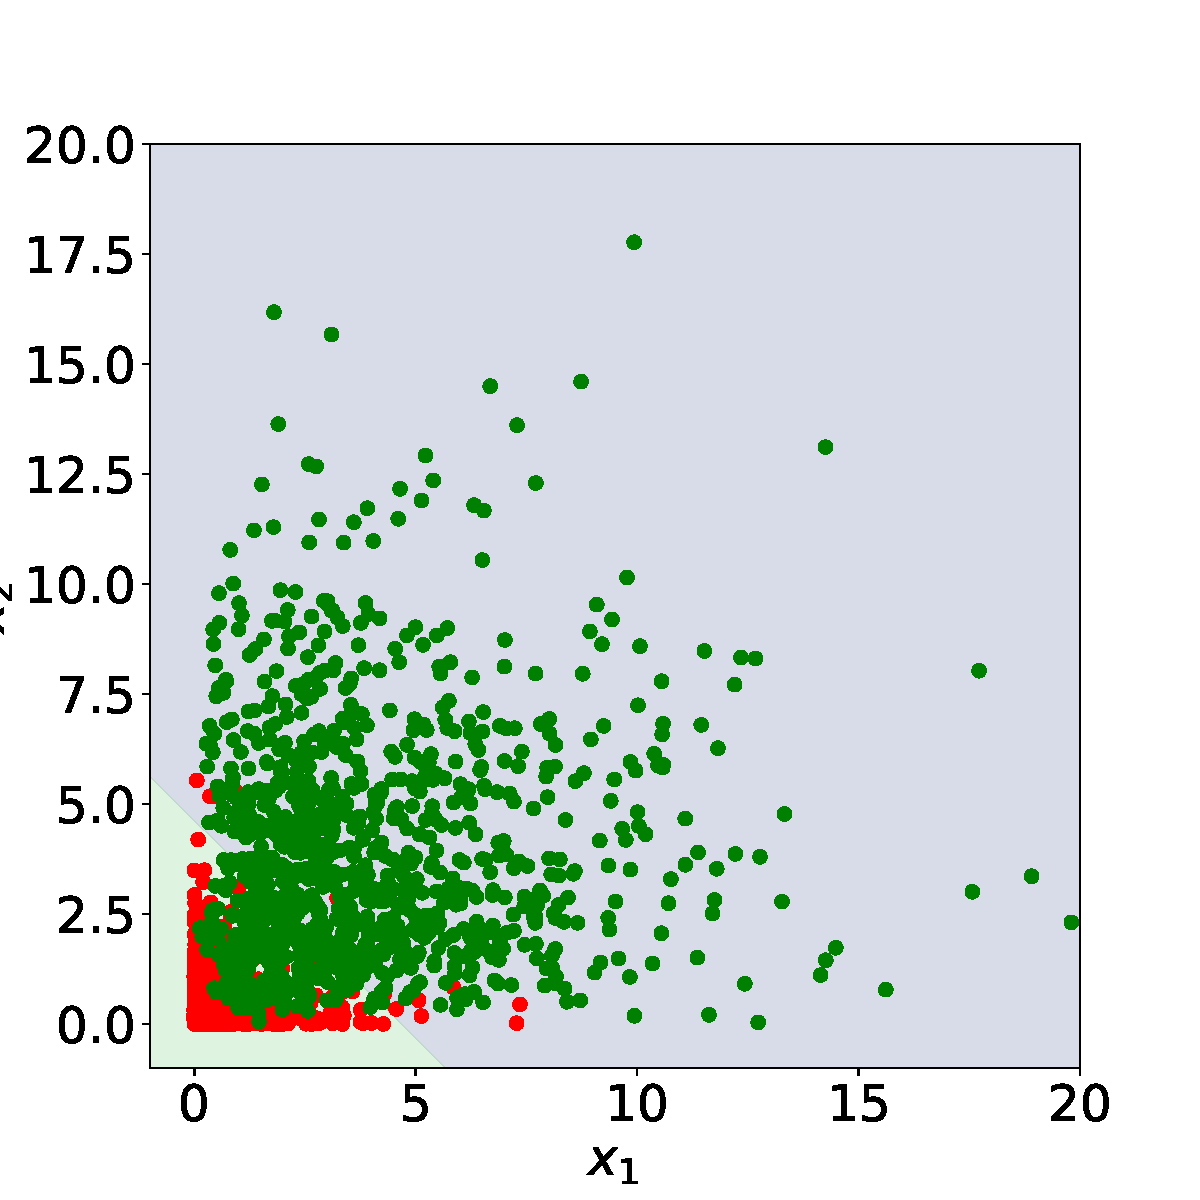
\includegraphics[width=1.5in]{../results/ex1/samples_LS_dataset_Gamma_size_10}}
\subfigure[LOG, Size $10$]{\label{fig:a}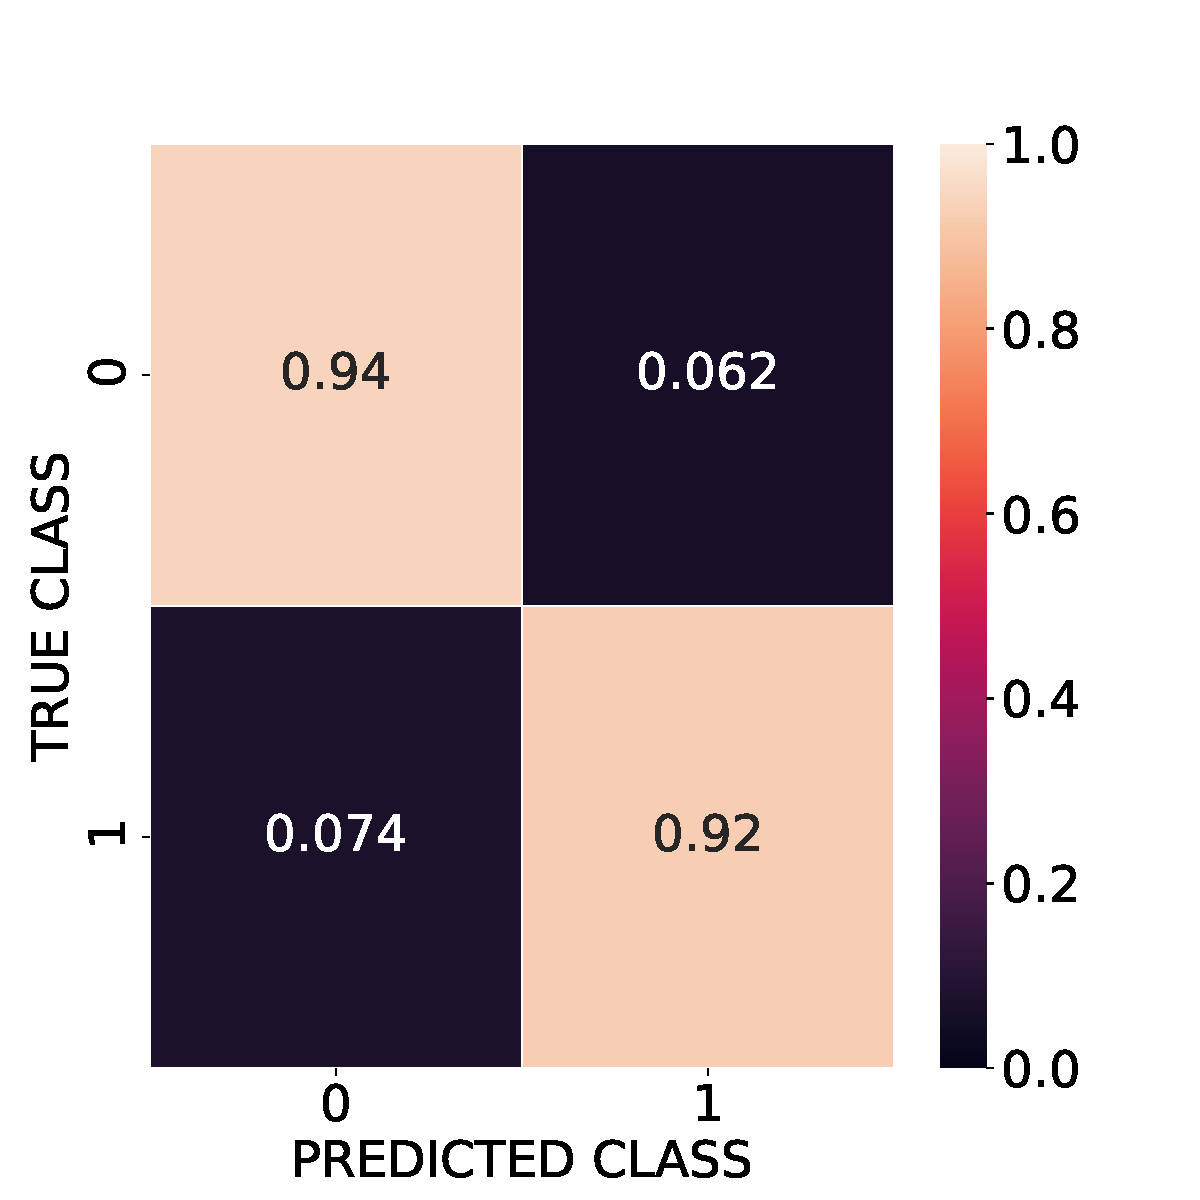
\includegraphics[width=1.5in]{../results/ex1/acc_LOG_dataset_Gamma_size_10}}
\subfigure[LOG Classifier]{\label{fig:a}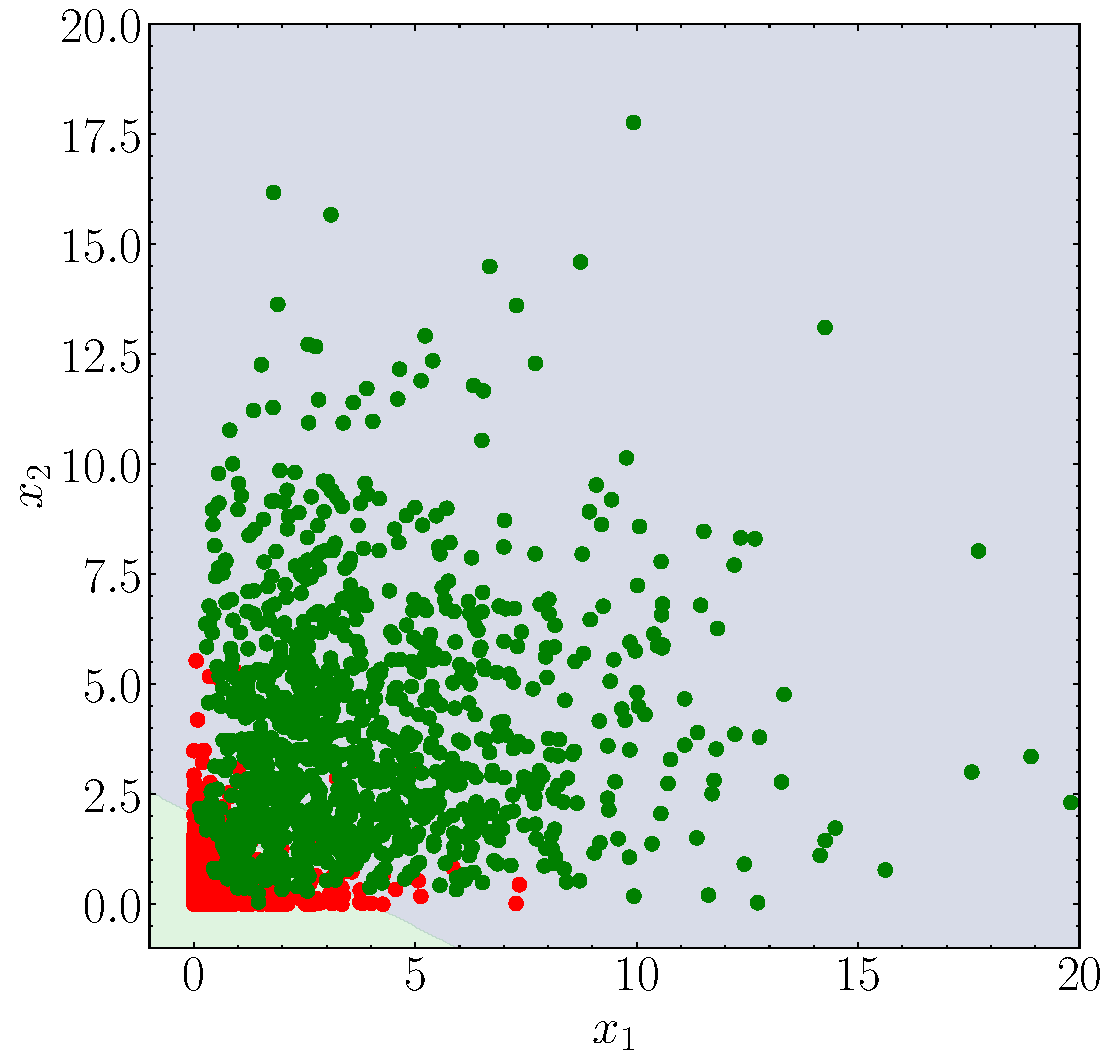
\includegraphics[width=1.5in]{../results/ex1/samples_LOG_dataset_Gamma_size_10}}

\subfigure[LS, Size $50$]{\label{fig:a}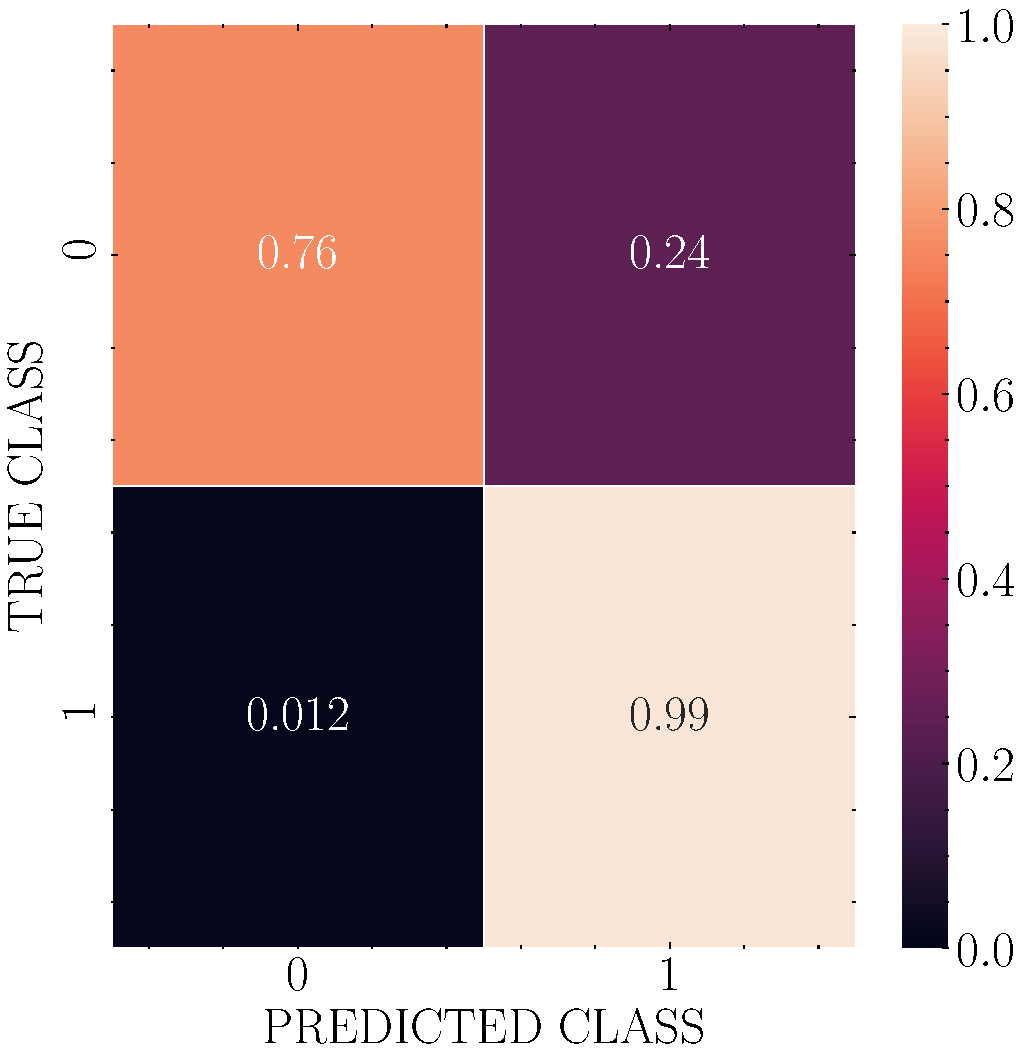
\includegraphics[width=1.5in]{../results/ex1/acc_LS_dataset_Gamma_size_50}}
\subfigure[LS Classifier]{\label{fig:a}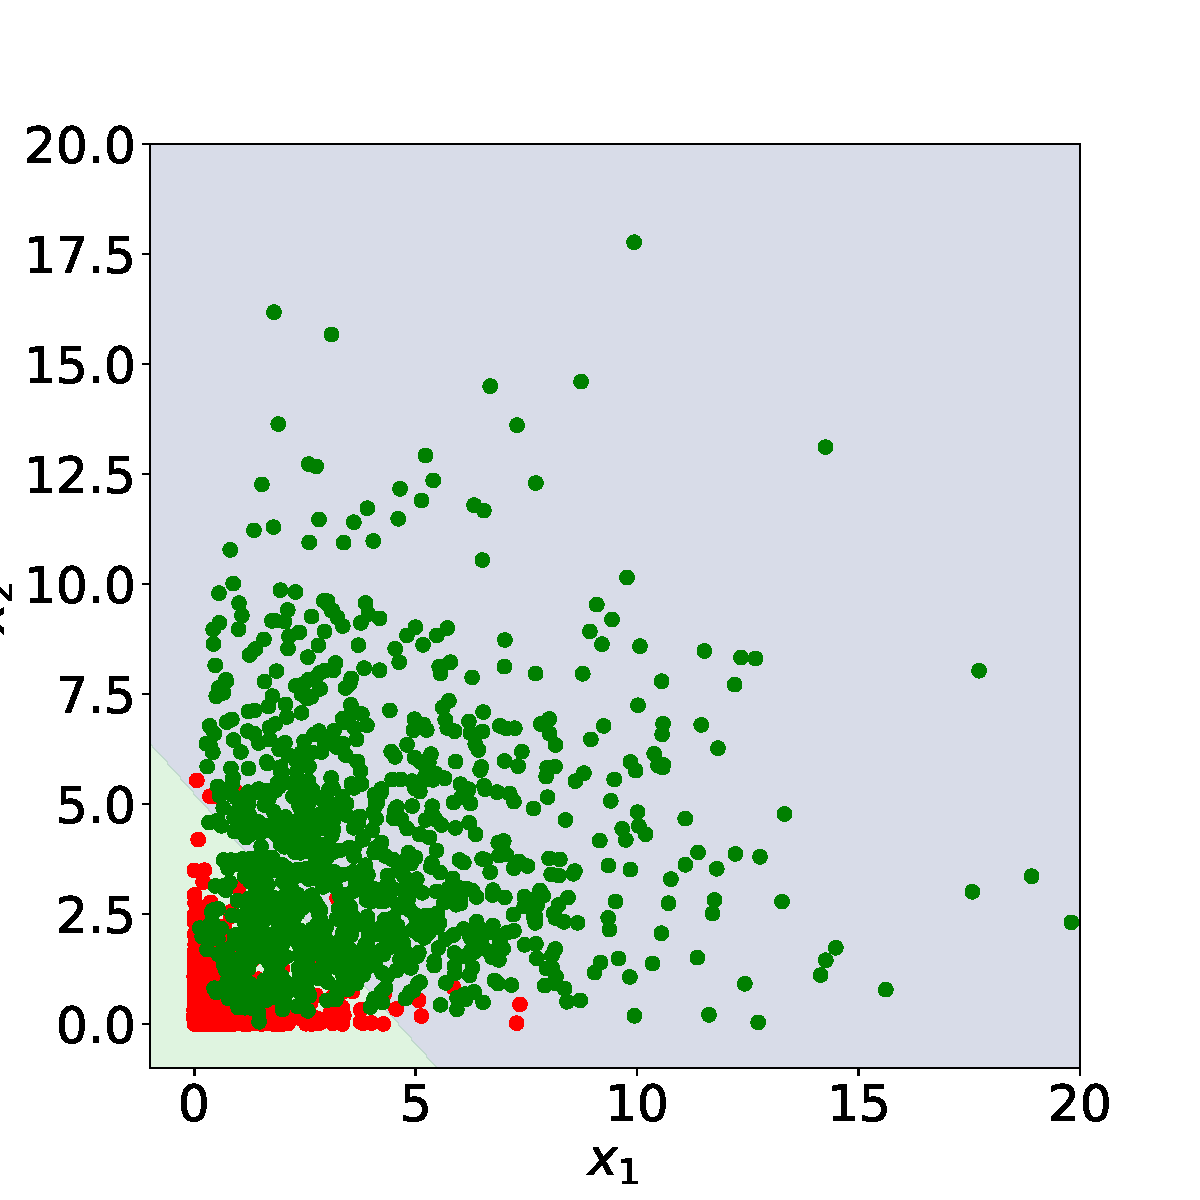
\includegraphics[width=1.5in]{../results/ex1/samples_LS_dataset_Gamma_size_50}}
\subfigure[LOG, Size $50$]{\label{fig:a}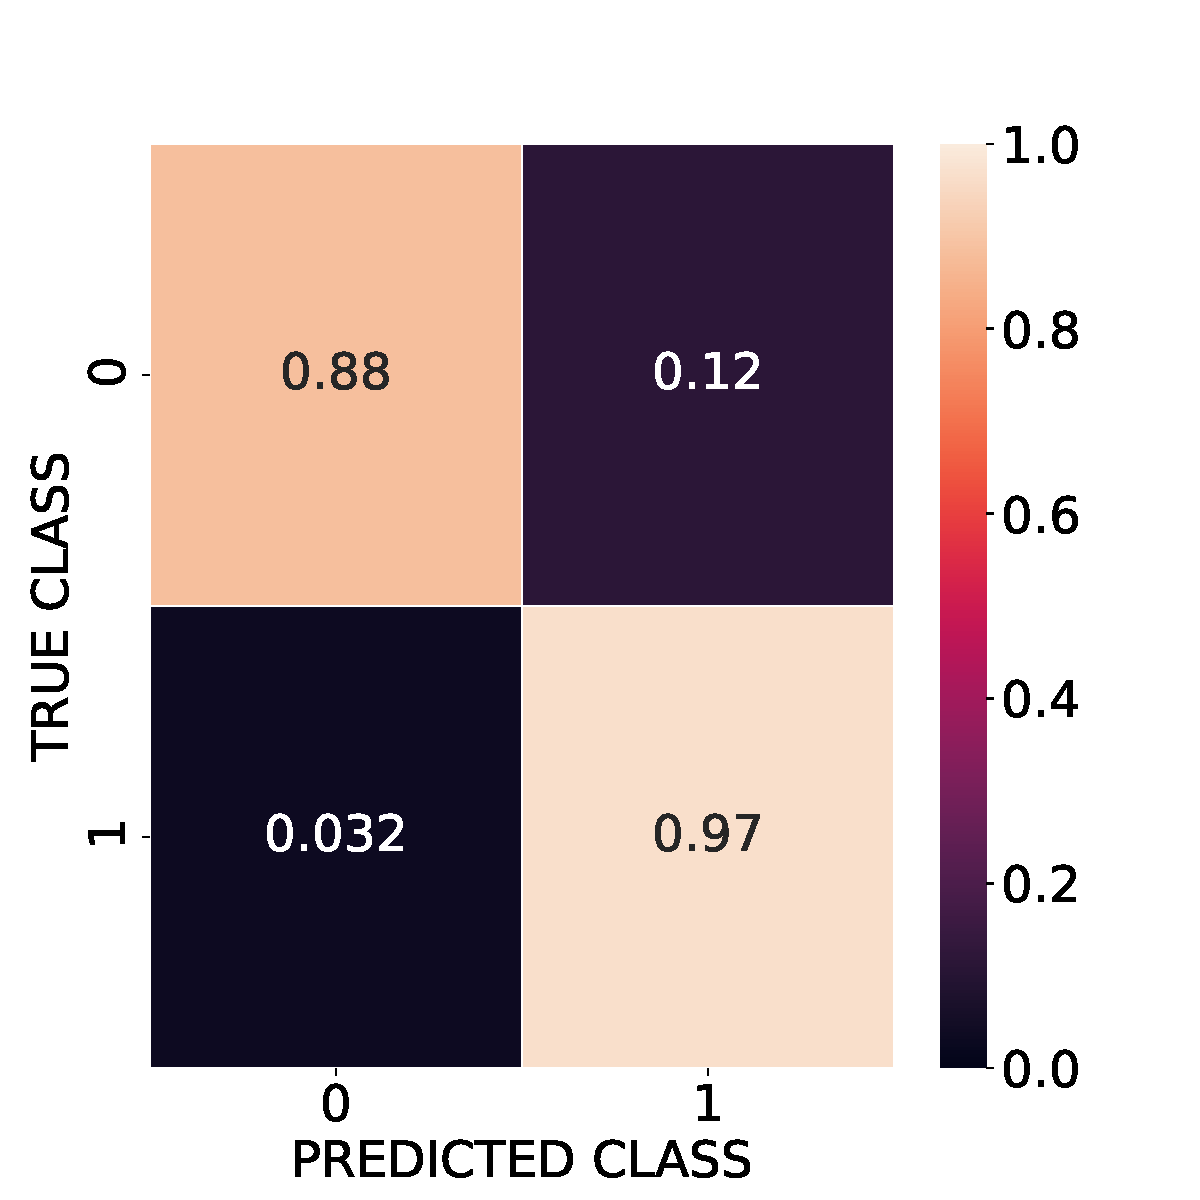
\includegraphics[width=1.5in]{../results/ex1/acc_LOG_dataset_Gamma_size_50}}
\subfigure[LOG Classifier]{\label{fig:a}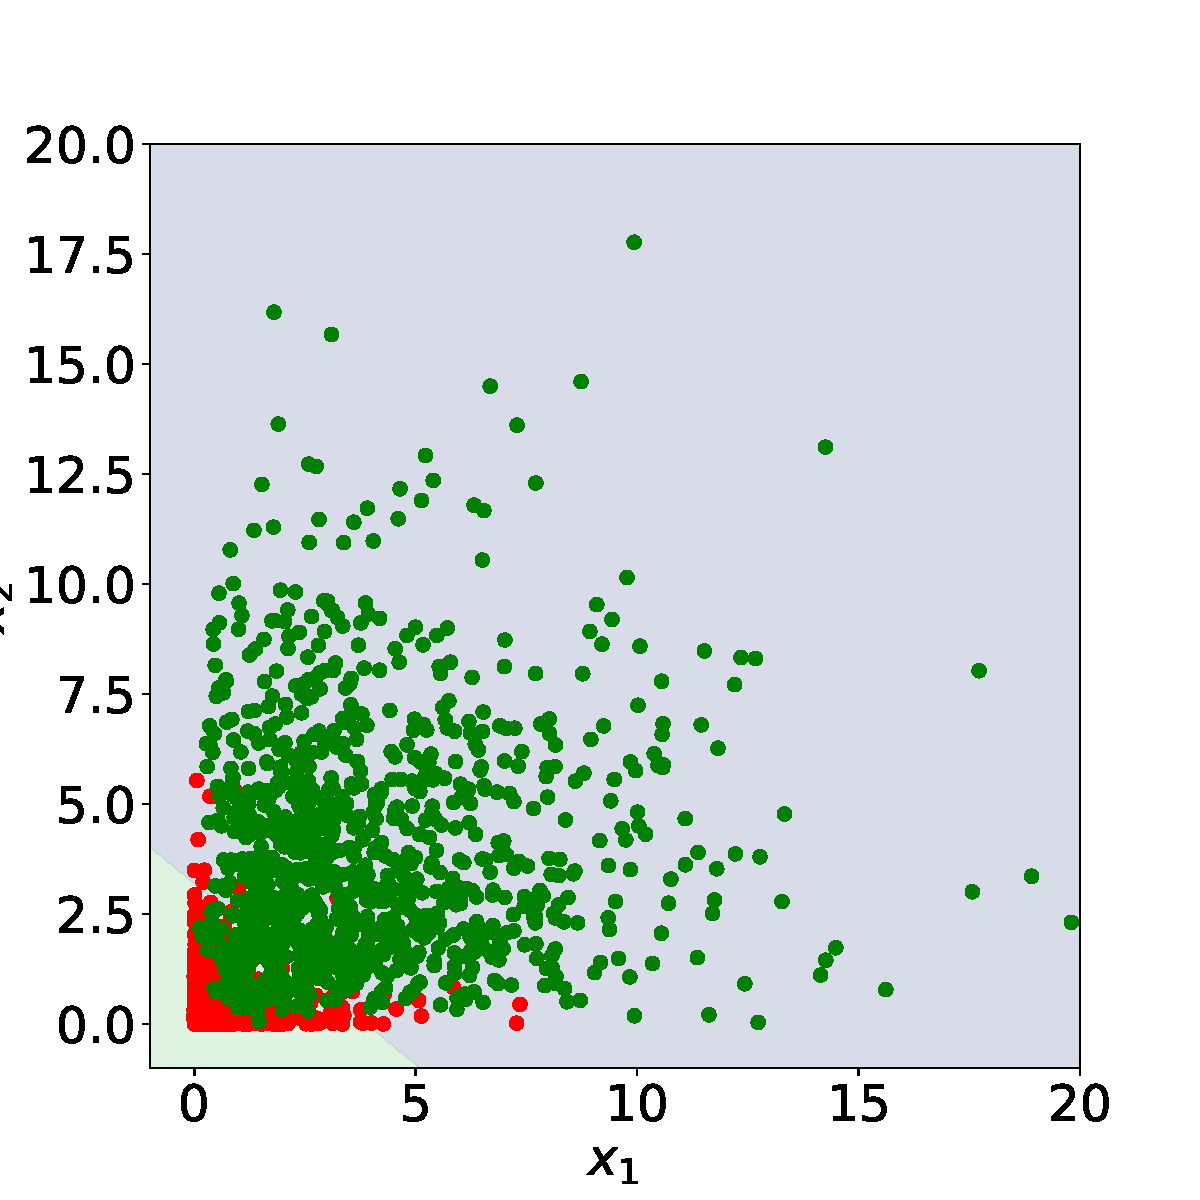
\includegraphics[width=1.5in]{../results/ex1/samples_LOG_dataset_Gamma_size_50}}

\subfigure[LS, Size $100$]{\label{fig:a}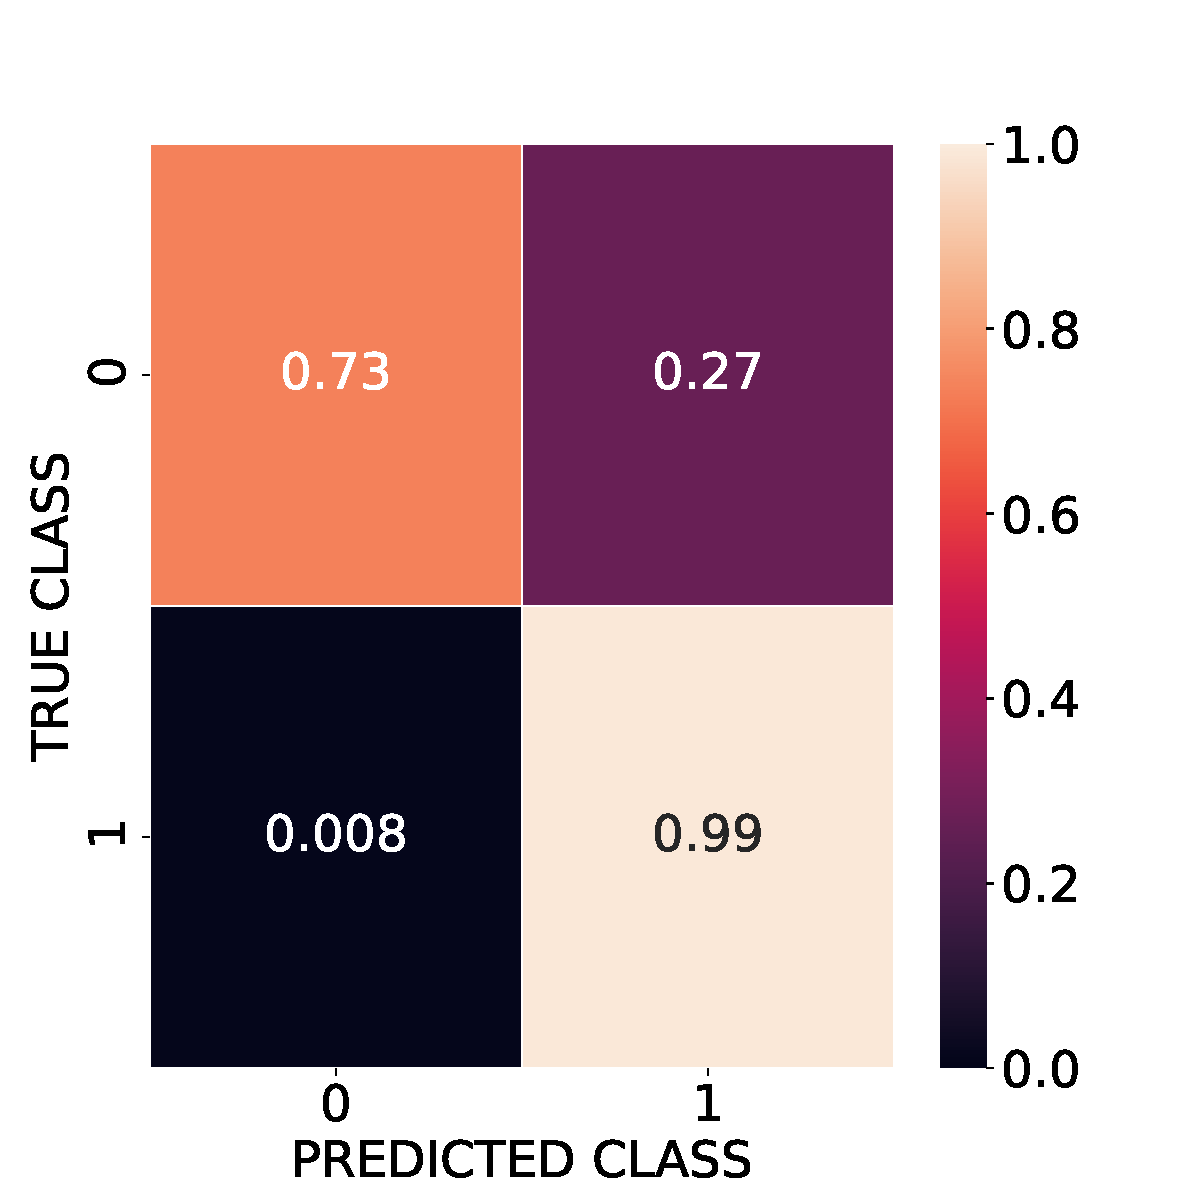
\includegraphics[width=1.5in]{../results/ex1/acc_LS_dataset_Gamma_size_100}}
\subfigure[LS Classifier]{\label{fig:a}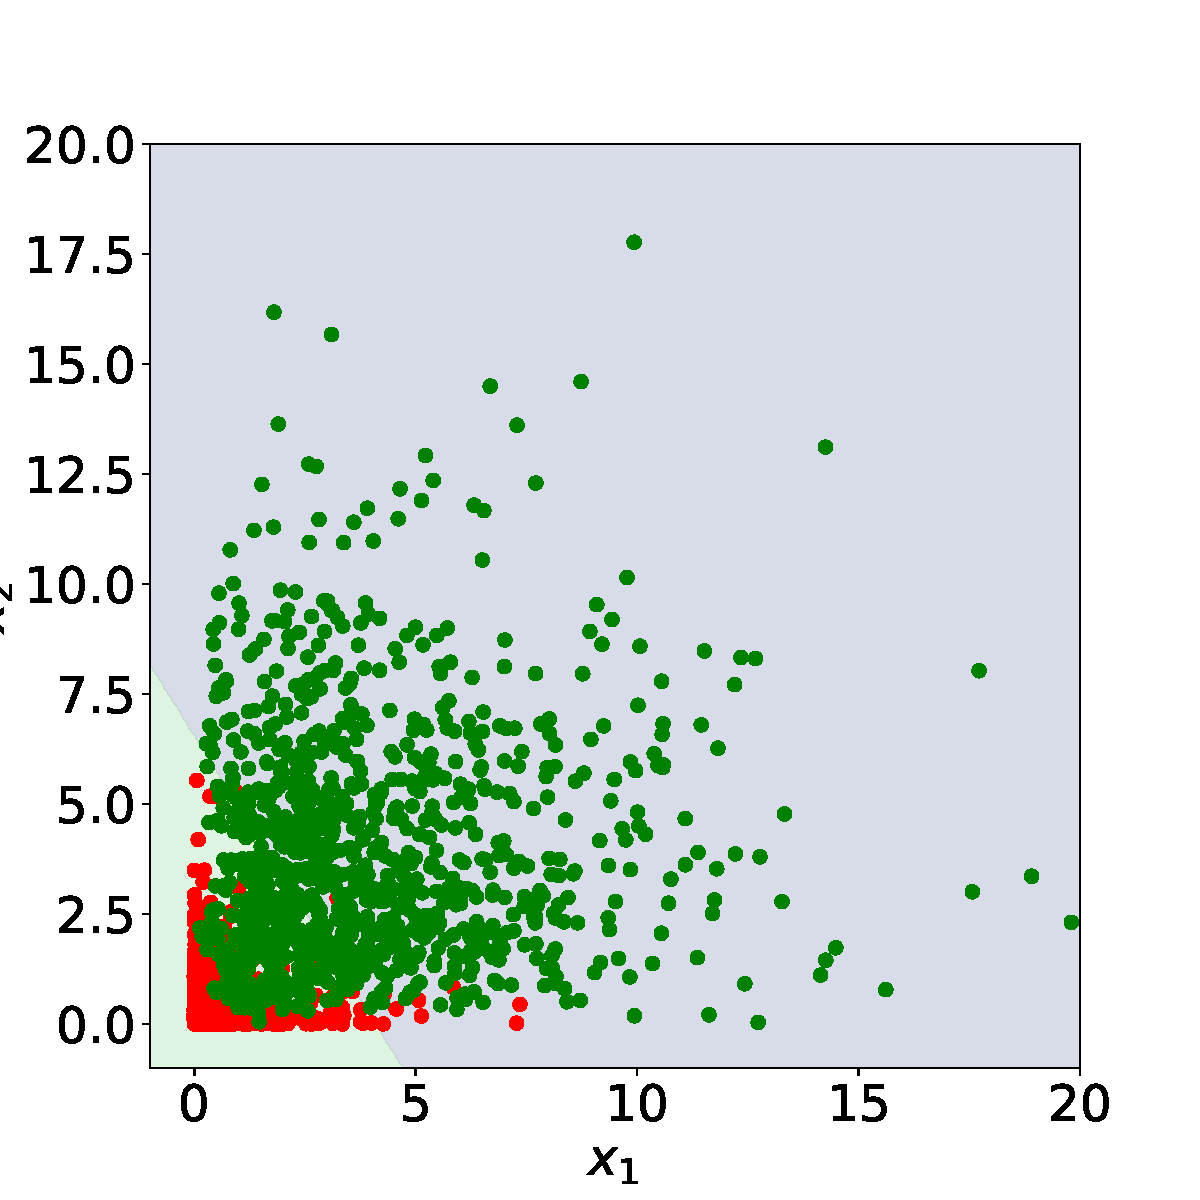
\includegraphics[width=1.5in]{../results/ex1/samples_LS_dataset_Gamma_size_100}}
\subfigure[LOG, Size $100$]{\label{fig:a}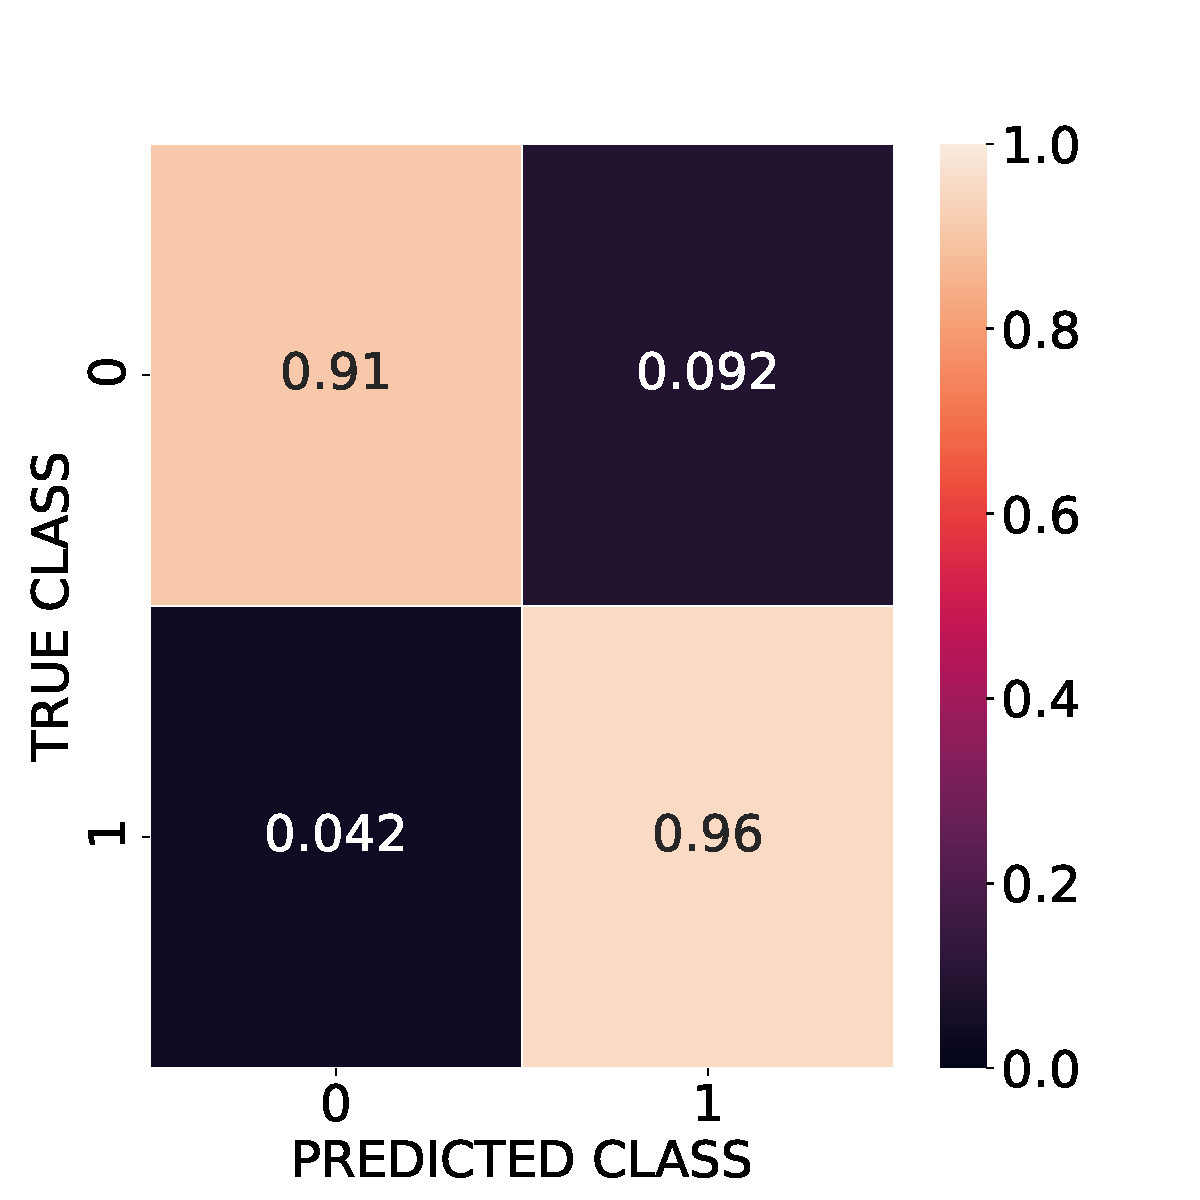
\includegraphics[width=1.5in]{../results/ex1/acc_LOG_dataset_Gamma_size_100}}
\subfigure[LOG Classifier]{\label{fig:a}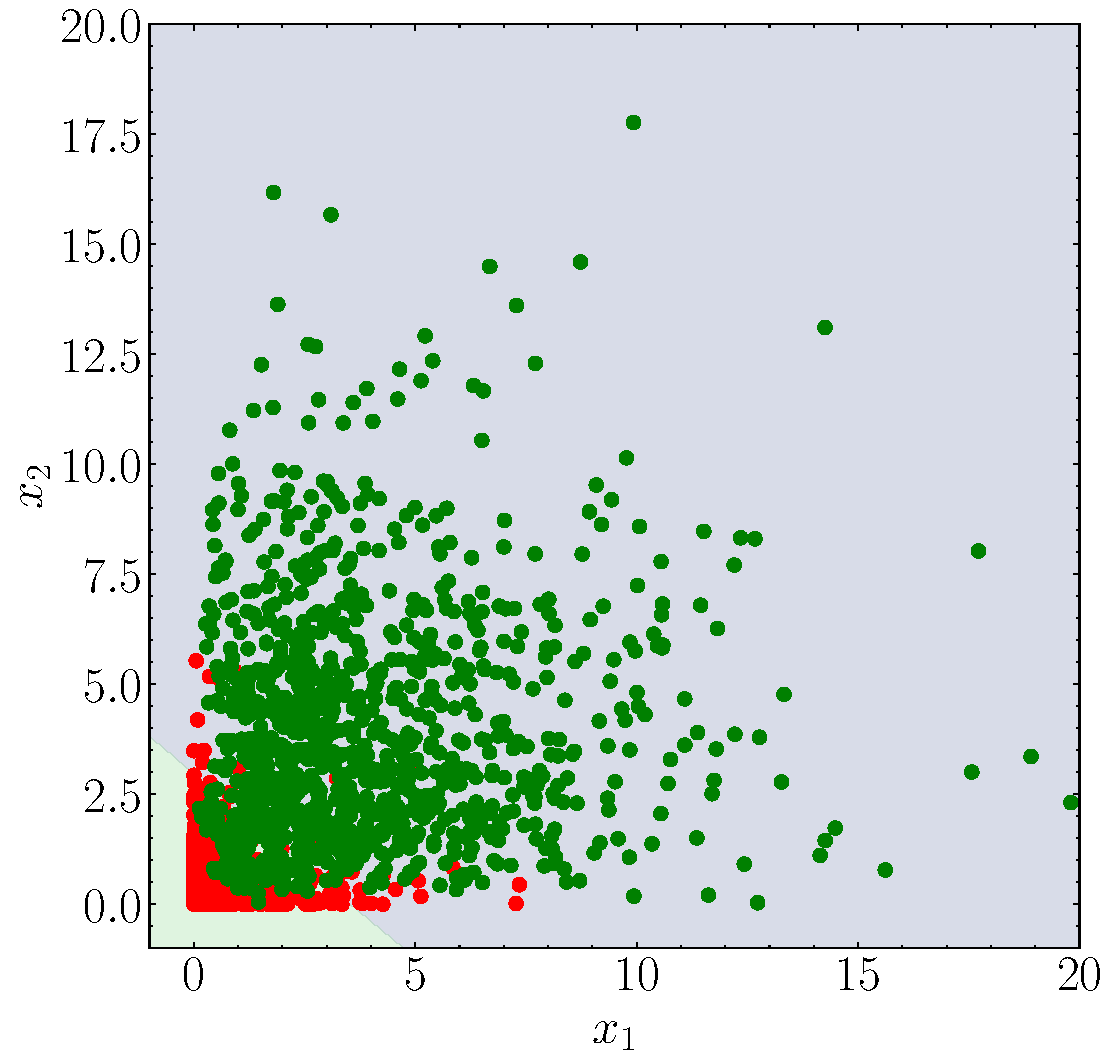
\includegraphics[width=1.5in]{../results/ex1/samples_LOG_dataset_Gamma_size_100}}

\subfigure[LS, Size $500$]{\label{fig:a}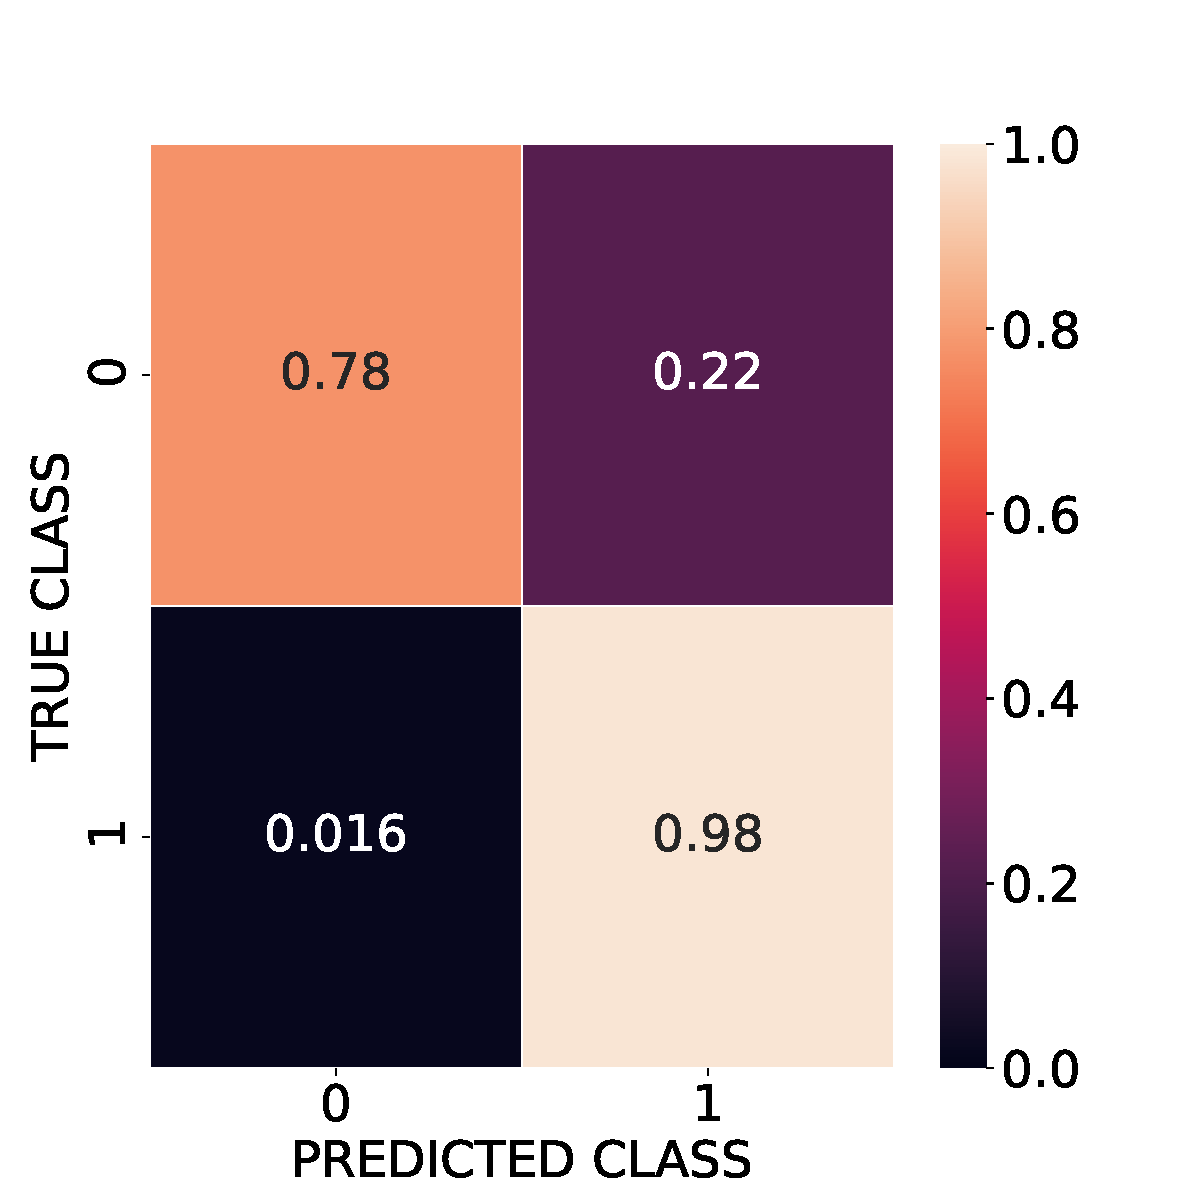
\includegraphics[width=1.5in]{../results/ex1/acc_LS_dataset_Gamma_size_500}}
\subfigure[LS Classifier]{\label{fig:a}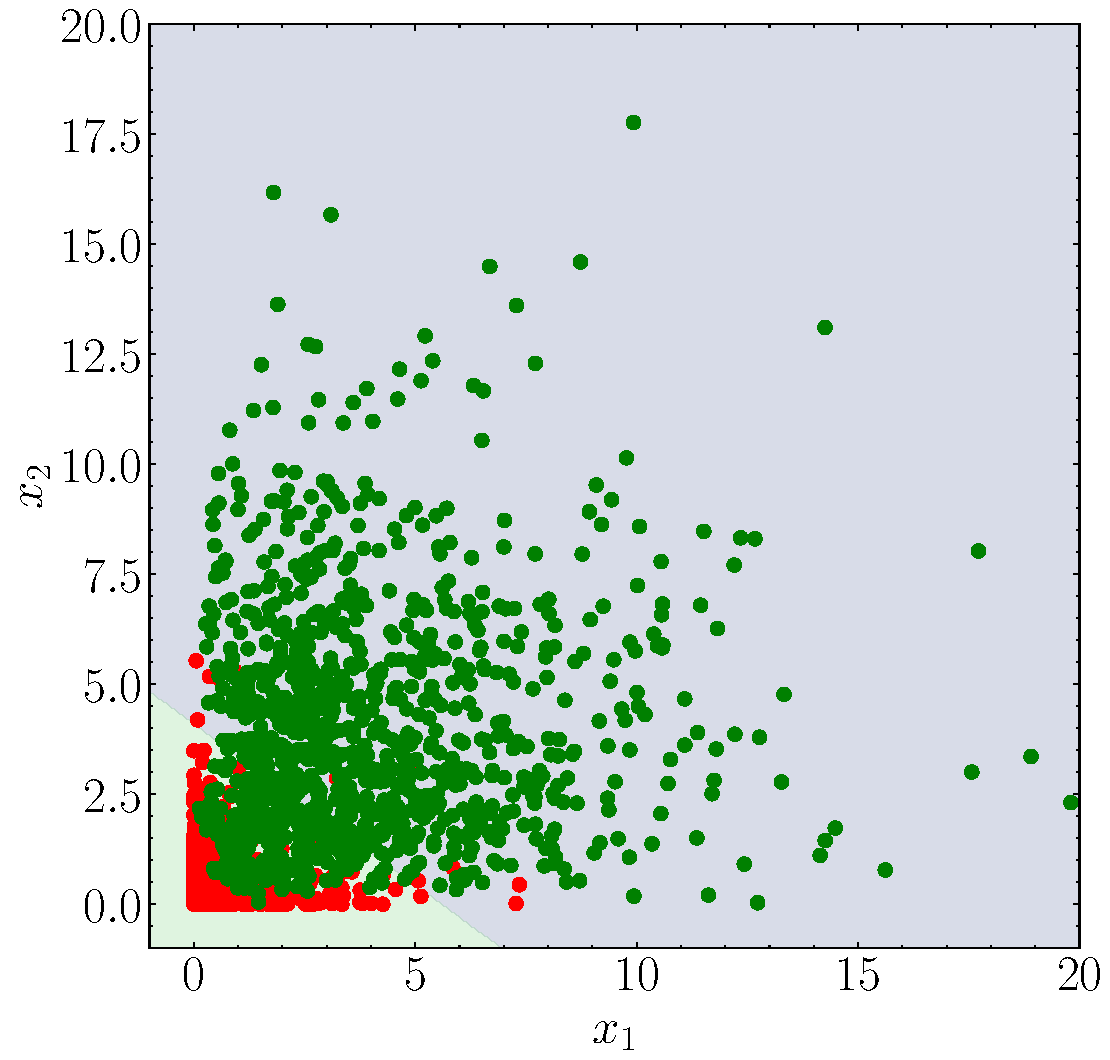
\includegraphics[width=1.5in]{../results/ex1/samples_LS_dataset_Gamma_size_500}}
\subfigure[LOG, Size $500$]{\label{fig:a}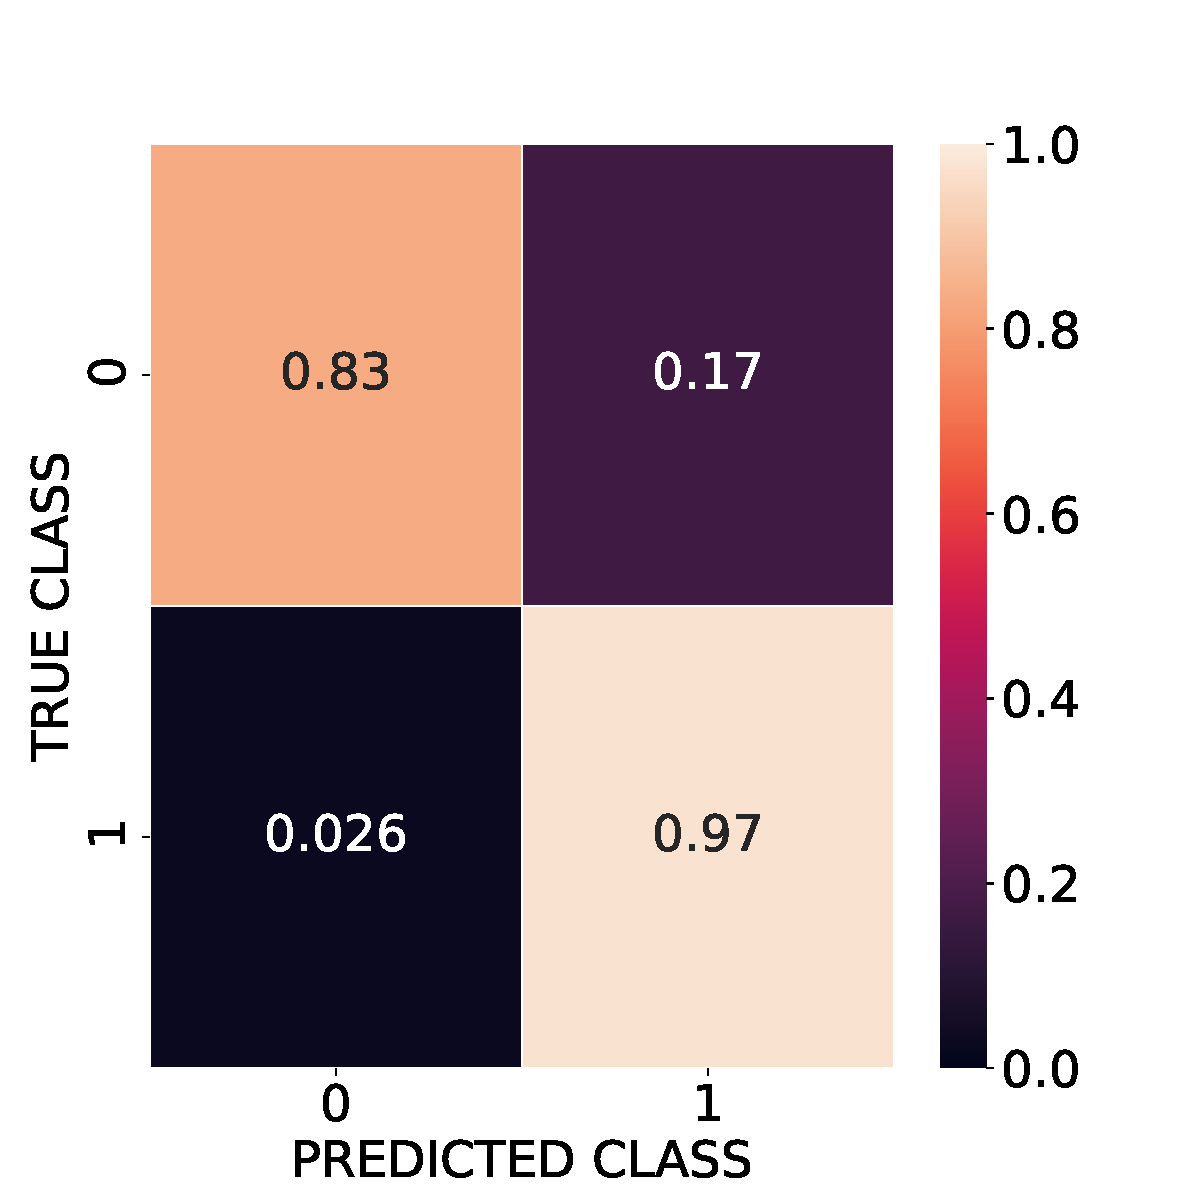
\includegraphics[width=1.5in]{../results/ex1/acc_LOG_dataset_Gamma_size_500}}
\subfigure[LOG Classifier]{\label{fig:a}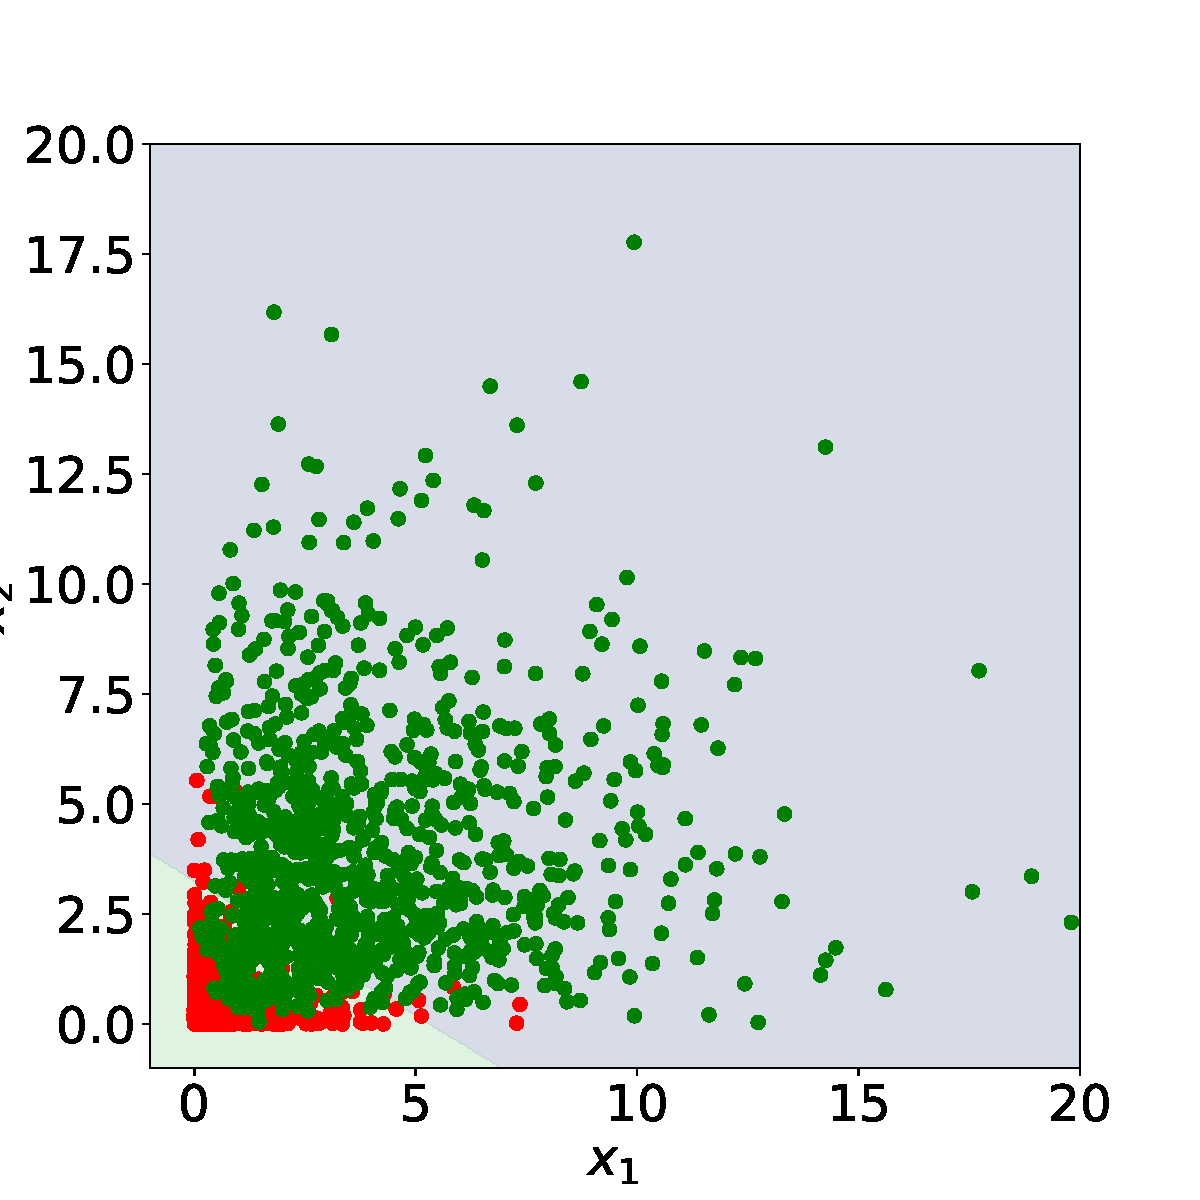
\includegraphics[width=1.5in]{../results/ex1/samples_LOG_dataset_Gamma_size_500}}

\subfigure[LS, Size $999$]{\label{fig:a}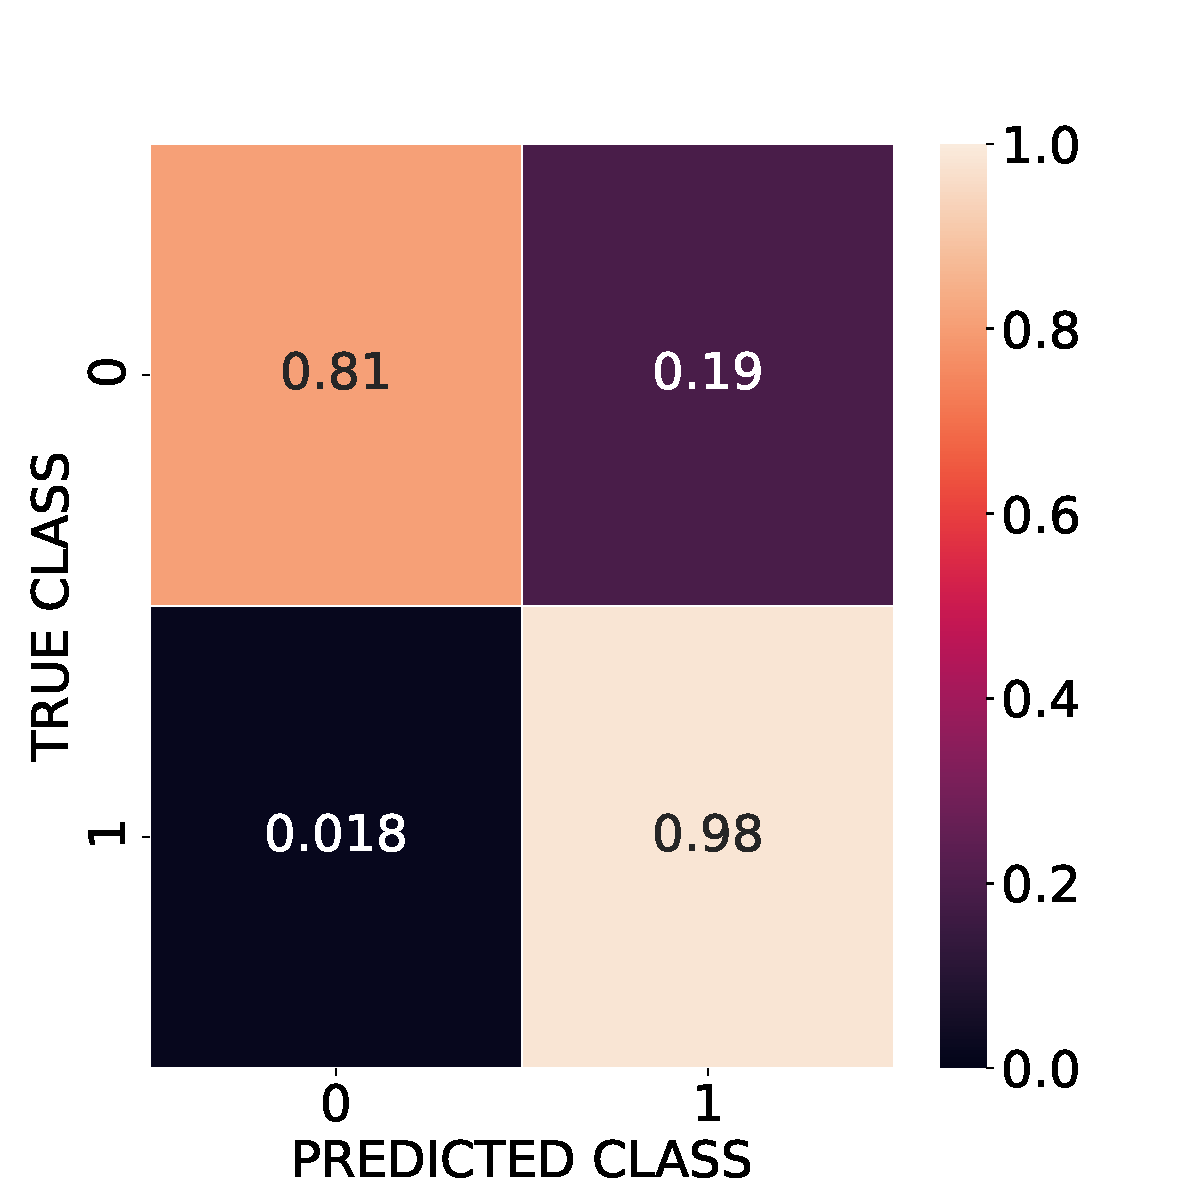
\includegraphics[width=1.5in]{../results/ex1/acc_LS_dataset_Gamma_size_999}}
\subfigure[LS Classifier]{\label{fig:a}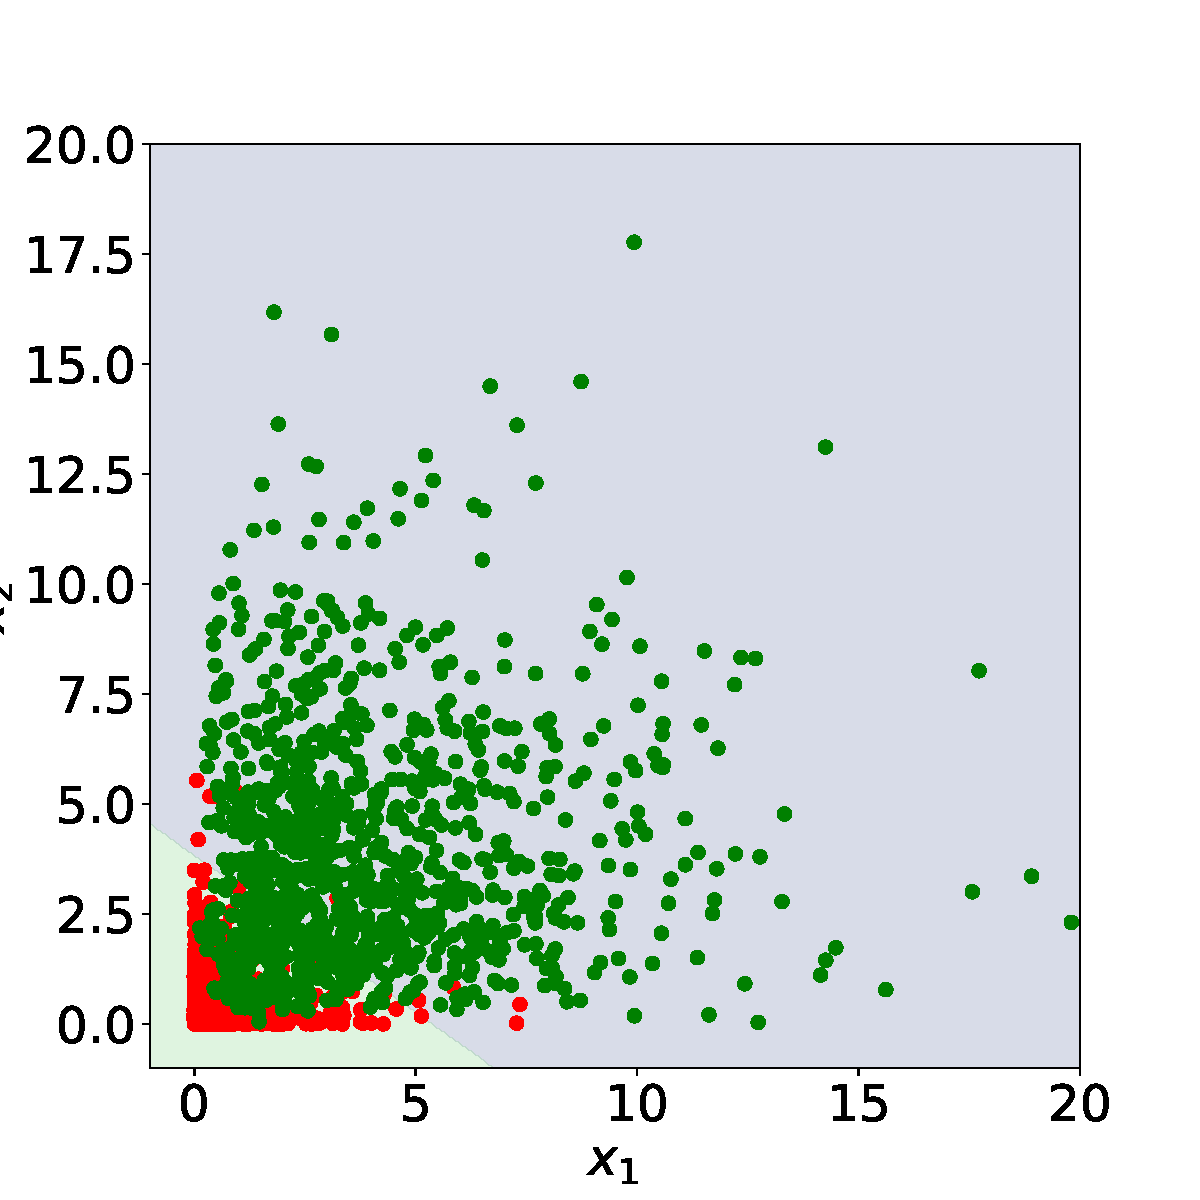
\includegraphics[width=1.5in]{../results/ex1/samples_LS_dataset_Gamma_size_999}}
\subfigure[LOG, Size $999$]{\label{fig:a}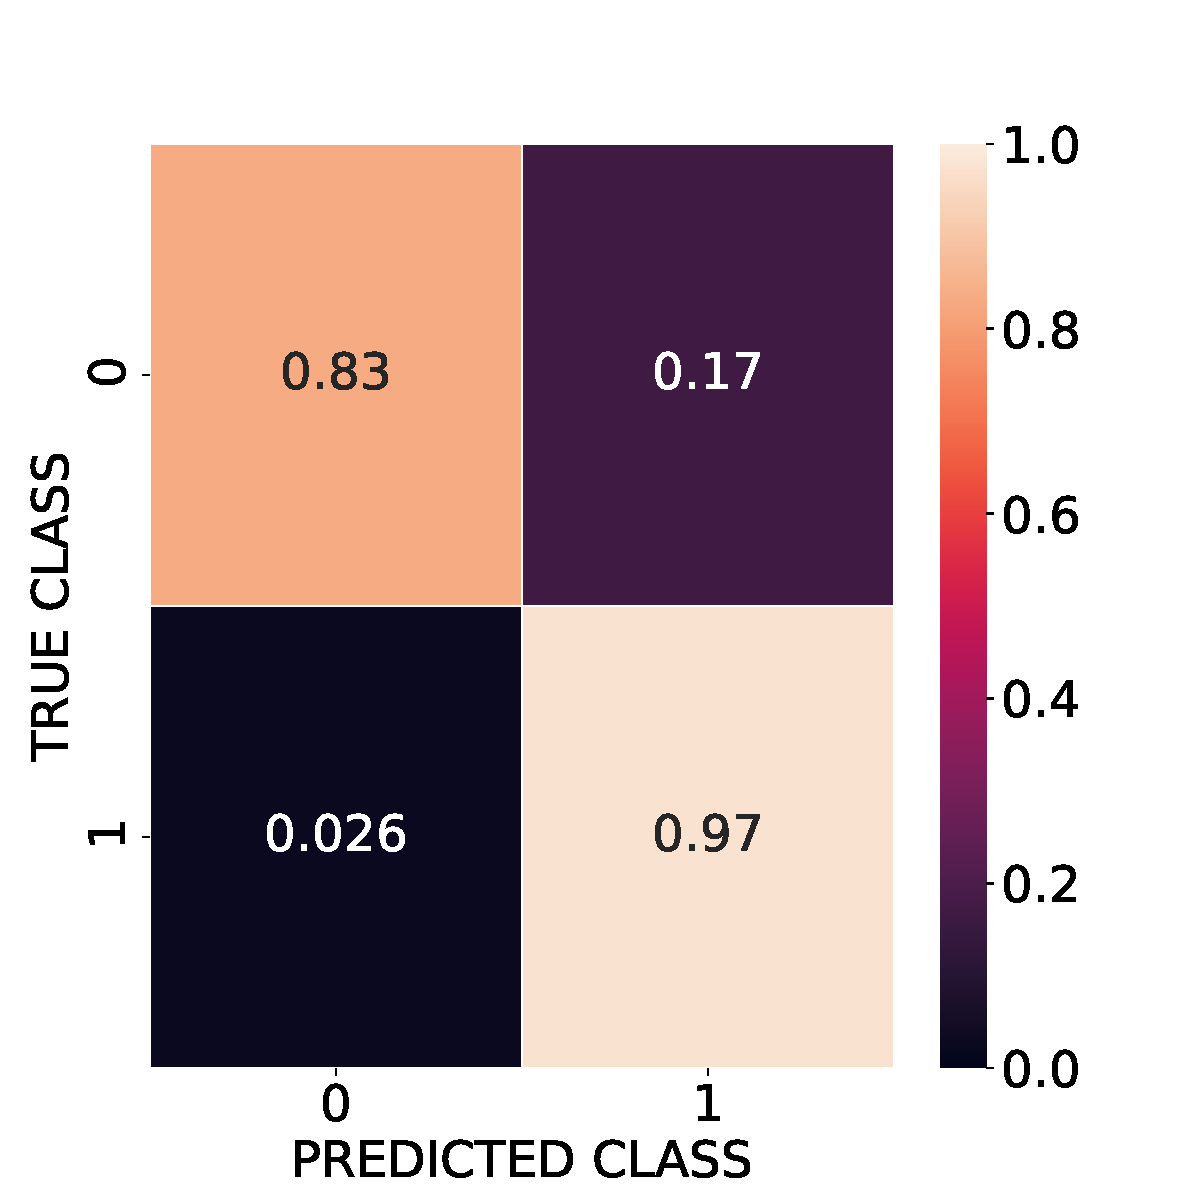
\includegraphics[width=1.5in]{../results/ex1/acc_LOG_dataset_Gamma_size_999}}
\subfigure[LOG Classifier]{\label{fig:a}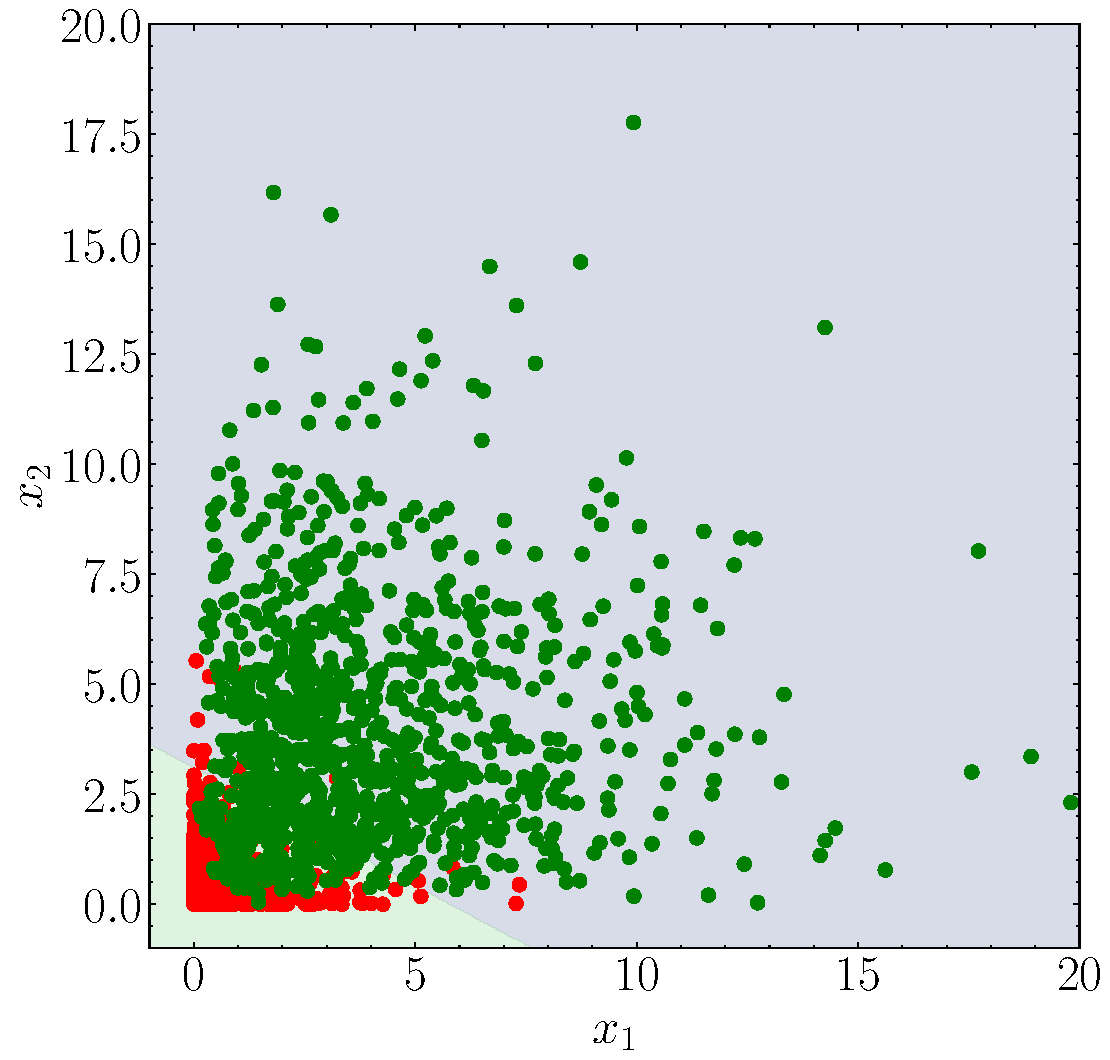
\includegraphics[width=1.5in]{../results/ex1/samples_LOG_dataset_Gamma_size_999}}

\caption{Linear Least-Squares Classifier and Logistic Regression on Gamma distributed data.}
\label{fig:LS_LOG_Gamma}
\end{figure}

{\it \bfseries Inferences:} It can be seen that the accuracy increases with increasing training size from $10$, $50$, $100$, $500$ and $999$ in both classifiers. Between the classifiers, logistic regression consistently gives better accuracy. Since the $x_{1}$ and $x_{2}$ coordinates are independent and Gamma distributed, it is known that the linear classifier has a slope of $-1$. It can be seen that logistic regression achieves this with fewer training samples. This is reflected in the accuracy. \\

% ------------------------------------------------------------------------------------------------------------------------------------------------------

\problem{Problem (1.b) Uniform-distributed Classes in 2D}
\label{prob:1.b}

Let the class conditionals be modelled as uniform distributions with different supports. The $2$-class linear least-squares (LS) classifier is trained by minimising (\ref{eq:lsClassifier}) and logistic regression (LOG) is trained using gradient descent with constant step-size using (\ref{eq:logGD}). \\

{\it \bfseries Results:} Figure \ref{fig:LS_LOG_Uniform} shows the accuracies of classification in confusion matrices and the samples along with the discriminant function. The first and third columns shows the confusion matrices of the linear classifier and logistic regression, respectively with varying training sizes. The second and fourth column shows the samples along with the discriminant function. The accuracies reported are averaged over $10000$ realisations and one of the discriminant functions is plotted. \\

\begin{figure}
\centering
\subfigure[LS, Size $10$]{\label{fig:a}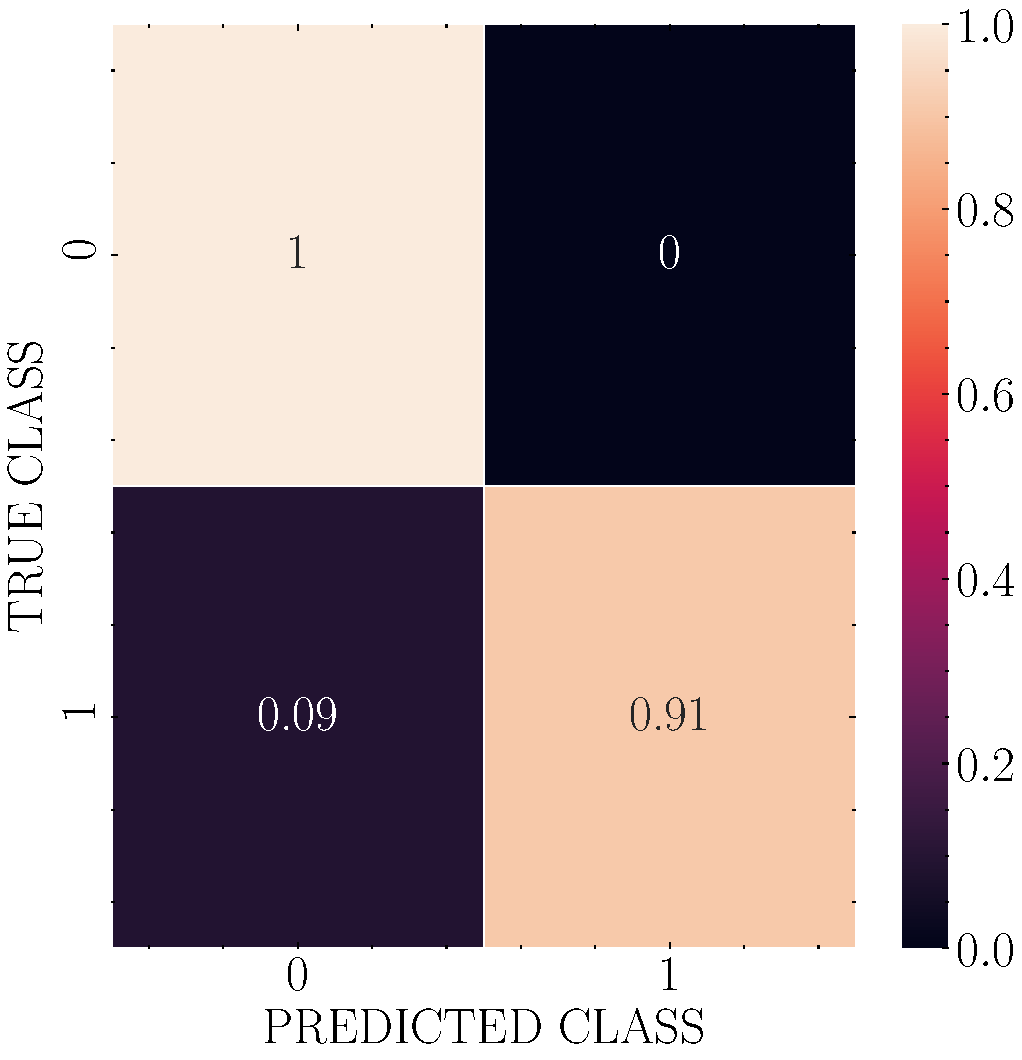
\includegraphics[width=1.5in]{../results/ex1/acc_LS_dataset_Uniform_size_10}}
\subfigure[LS Classifier]{\label{fig:a}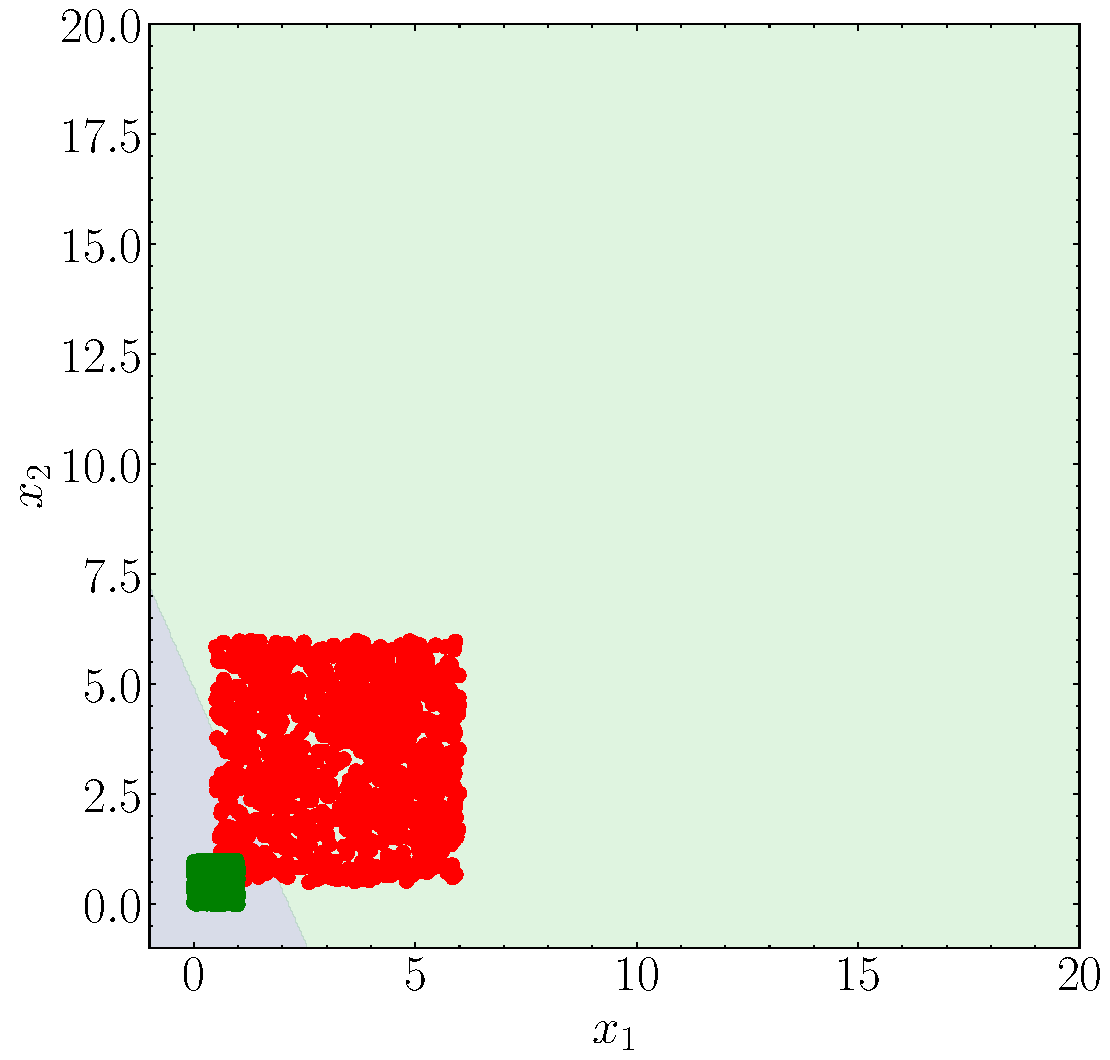
\includegraphics[width=1.5in]{../results/ex1/samples_LS_dataset_Uniform_size_10}}
\subfigure[LOG, Size $10$]{\label{fig:a}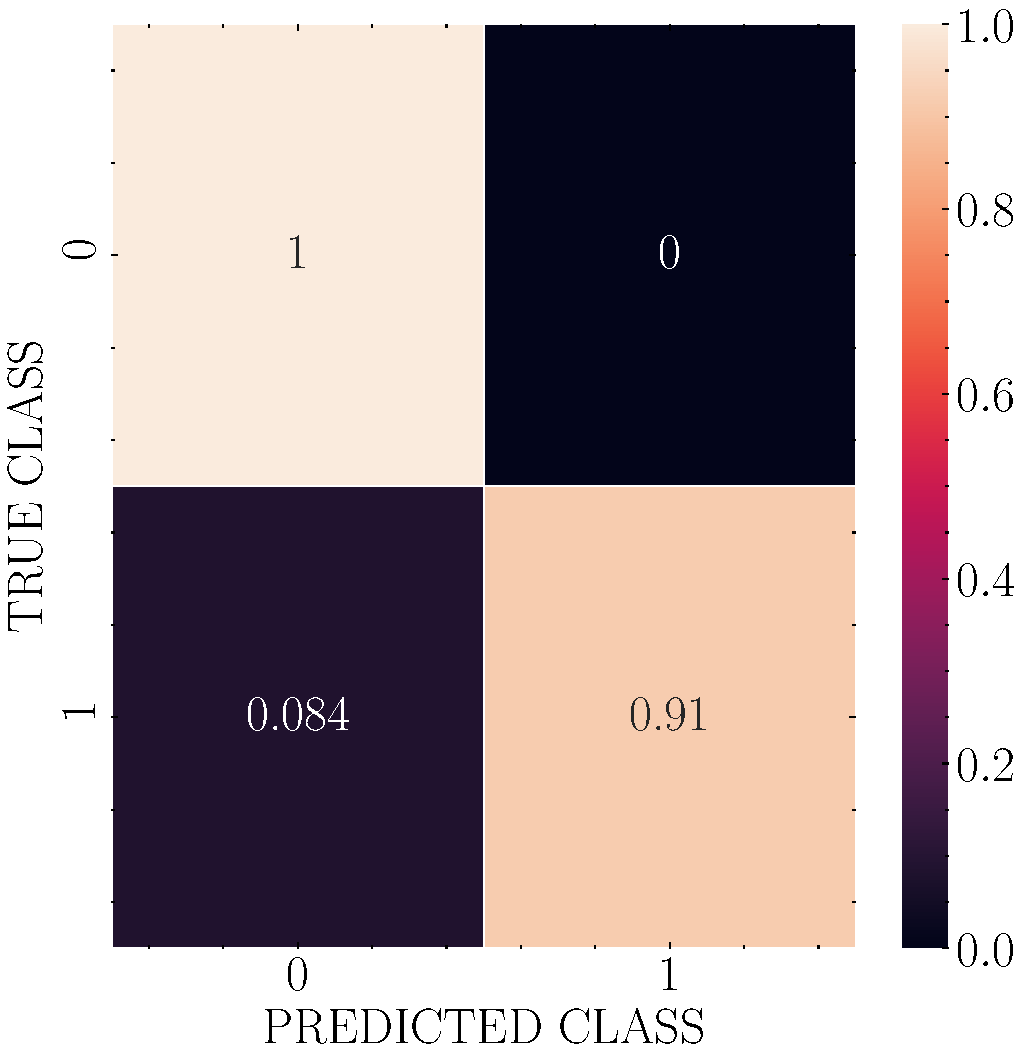
\includegraphics[width=1.5in]{../results/ex1/acc_LOG_dataset_Uniform_size_10}}
\subfigure[LOG Classifier]{\label{fig:a}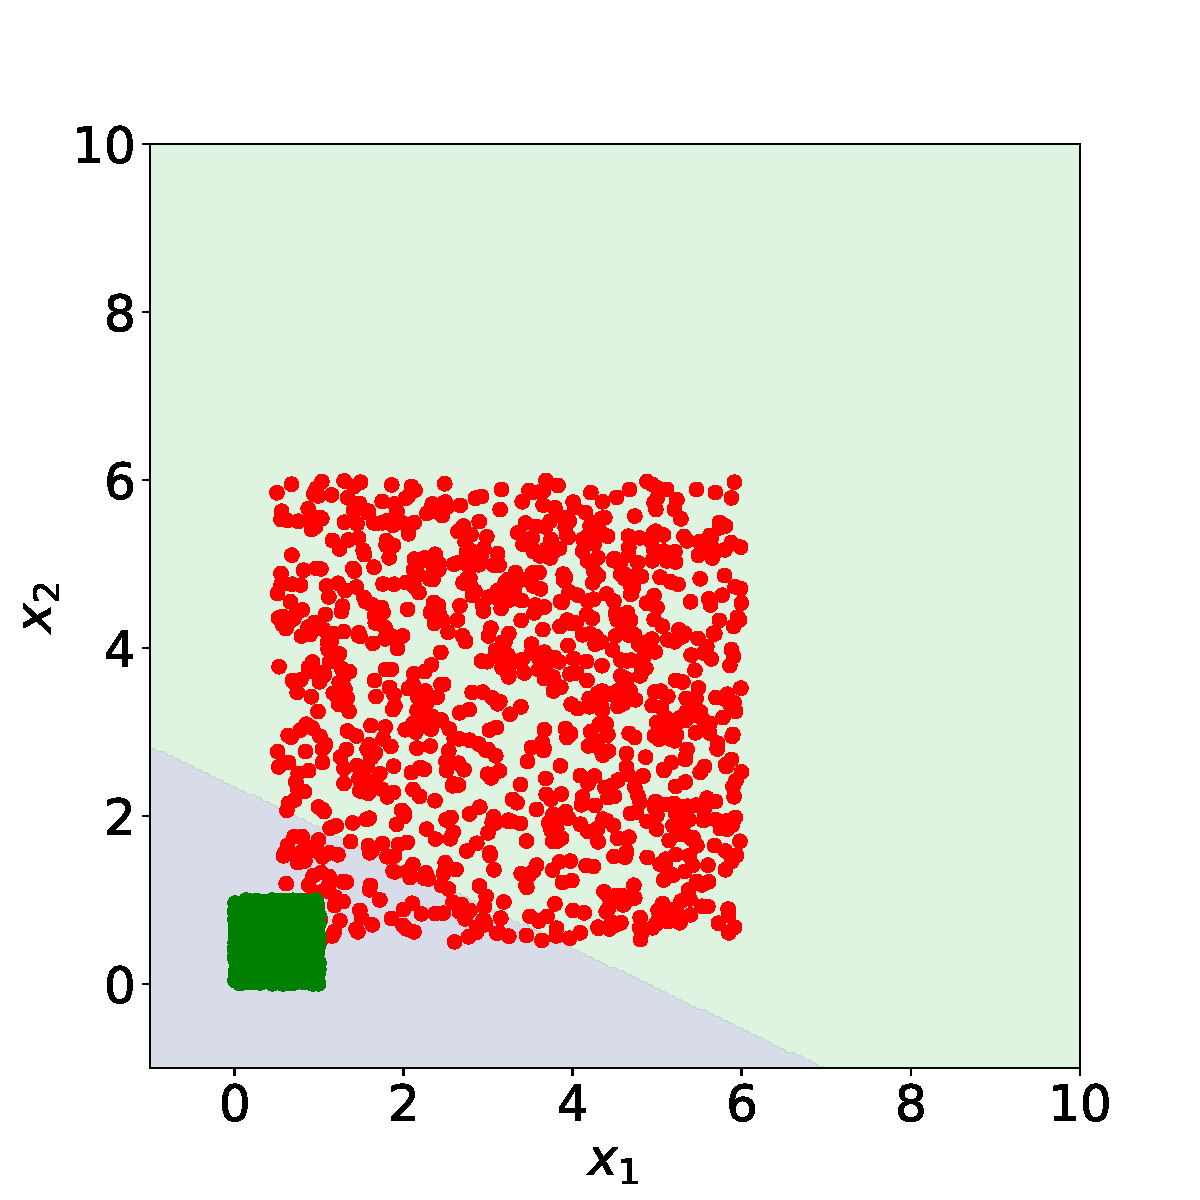
\includegraphics[width=1.5in]{../results/ex1/samples_LOG_dataset_Uniform_size_10}}

\subfigure[LS, Size $50$]{\label{fig:a}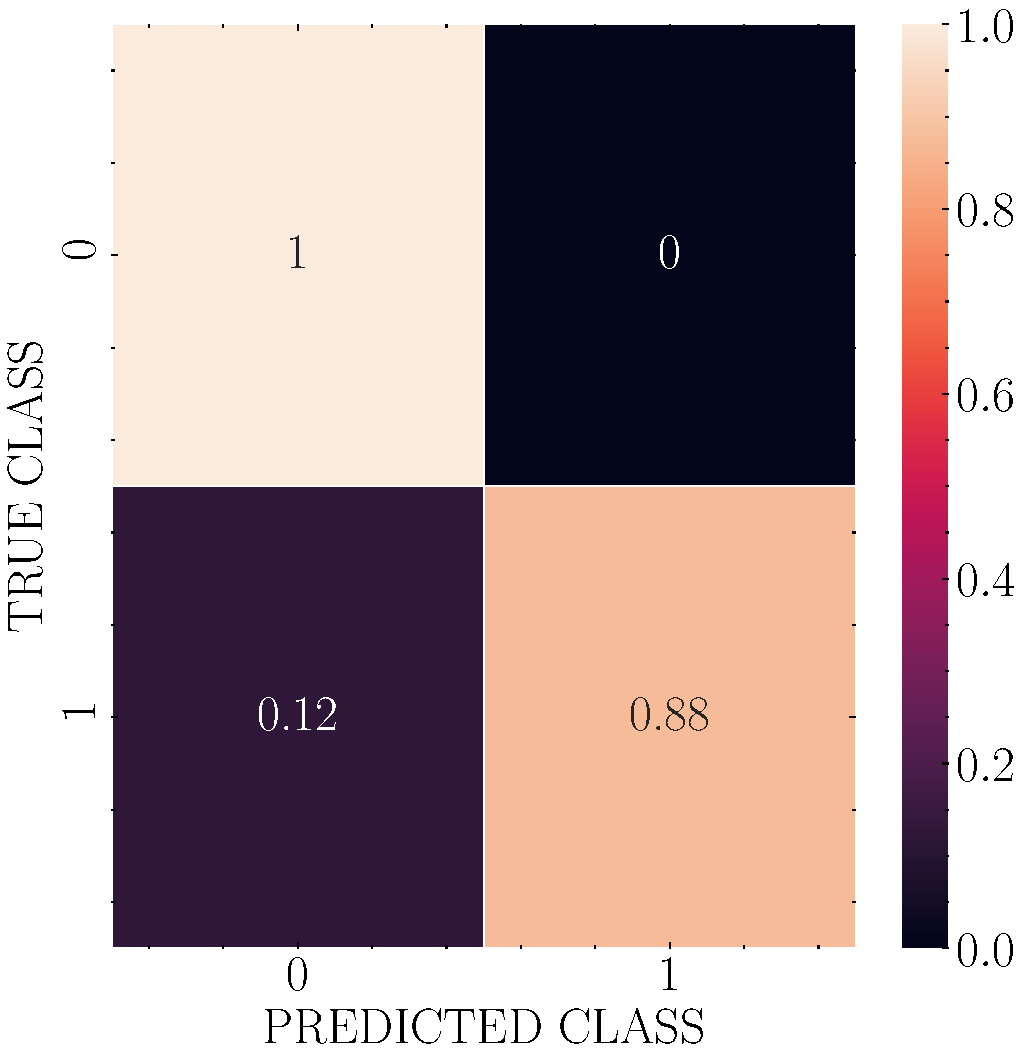
\includegraphics[width=1.5in]{../results/ex1/acc_LS_dataset_Uniform_size_50}}
\subfigure[LS Classifier]{\label{fig:a}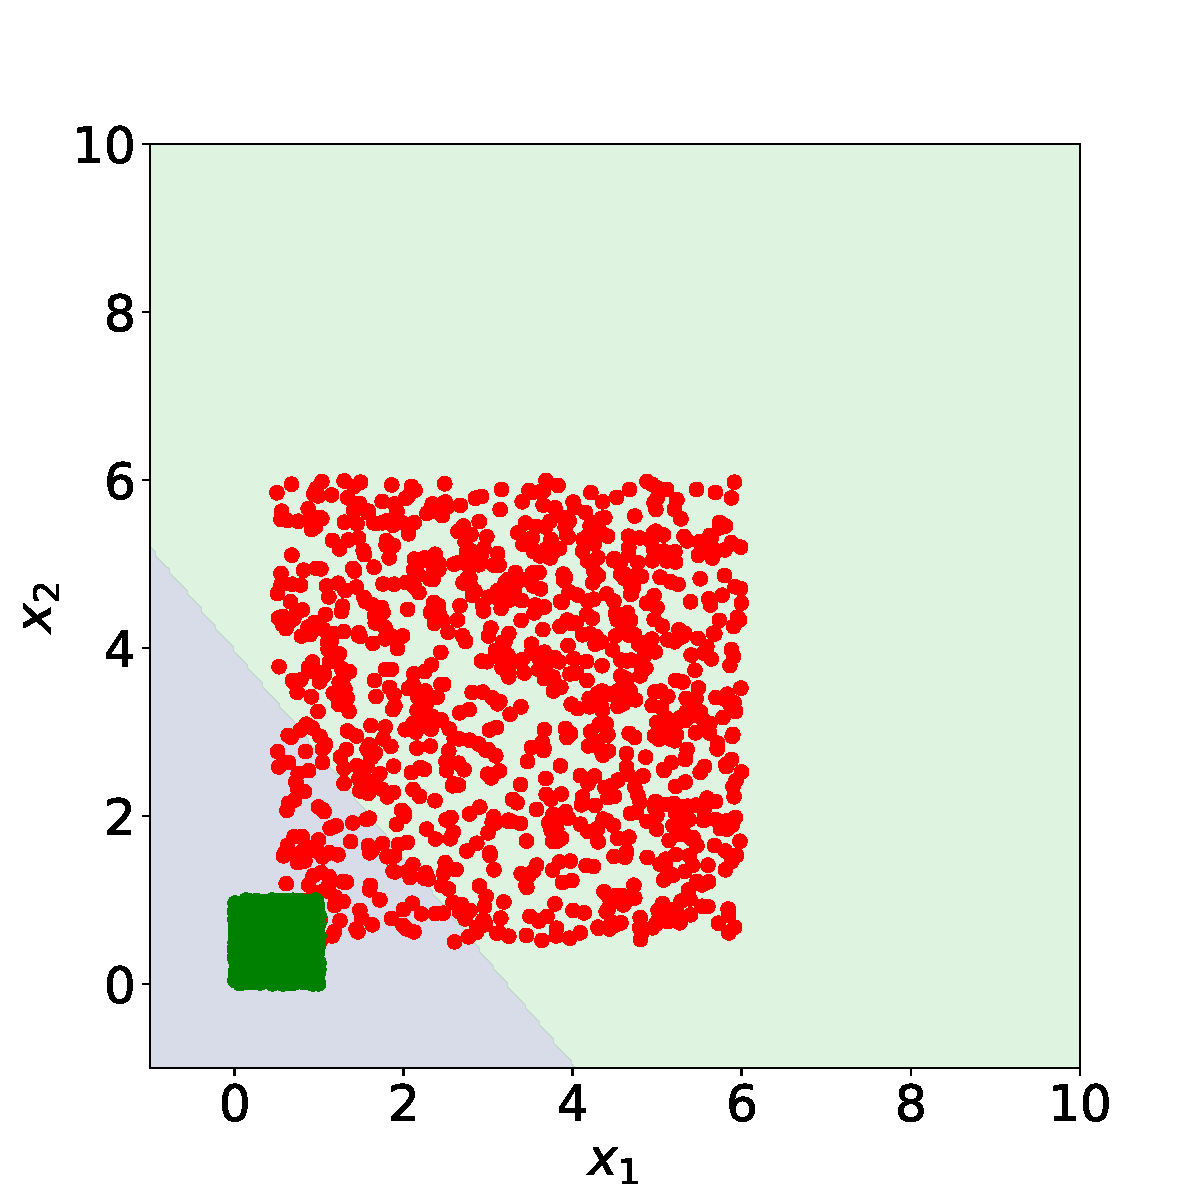
\includegraphics[width=1.5in]{../results/ex1/samples_LS_dataset_Uniform_size_50}}
\subfigure[LOG, Size $50$]{\label{fig:a}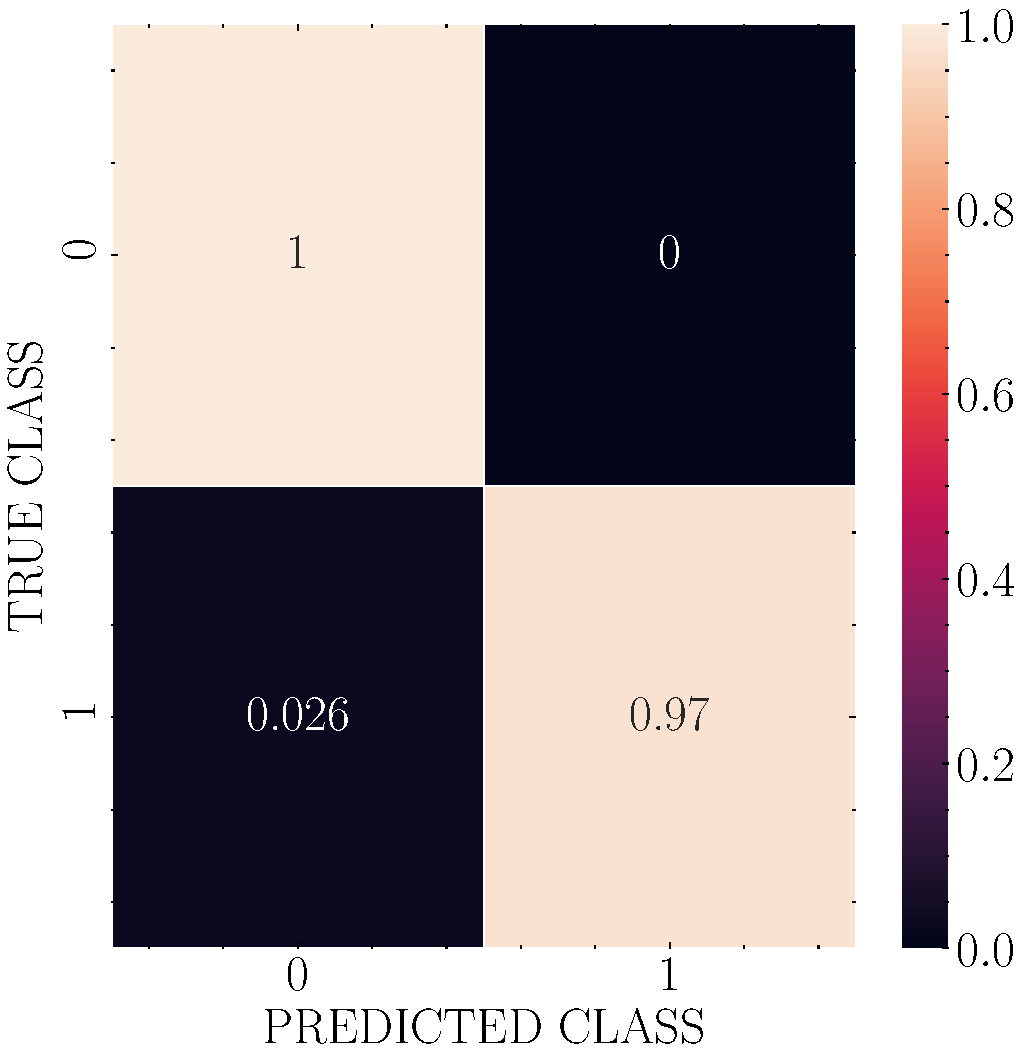
\includegraphics[width=1.5in]{../results/ex1/acc_LOG_dataset_Uniform_size_50}}
\subfigure[LOG Classifier]{\label{fig:a}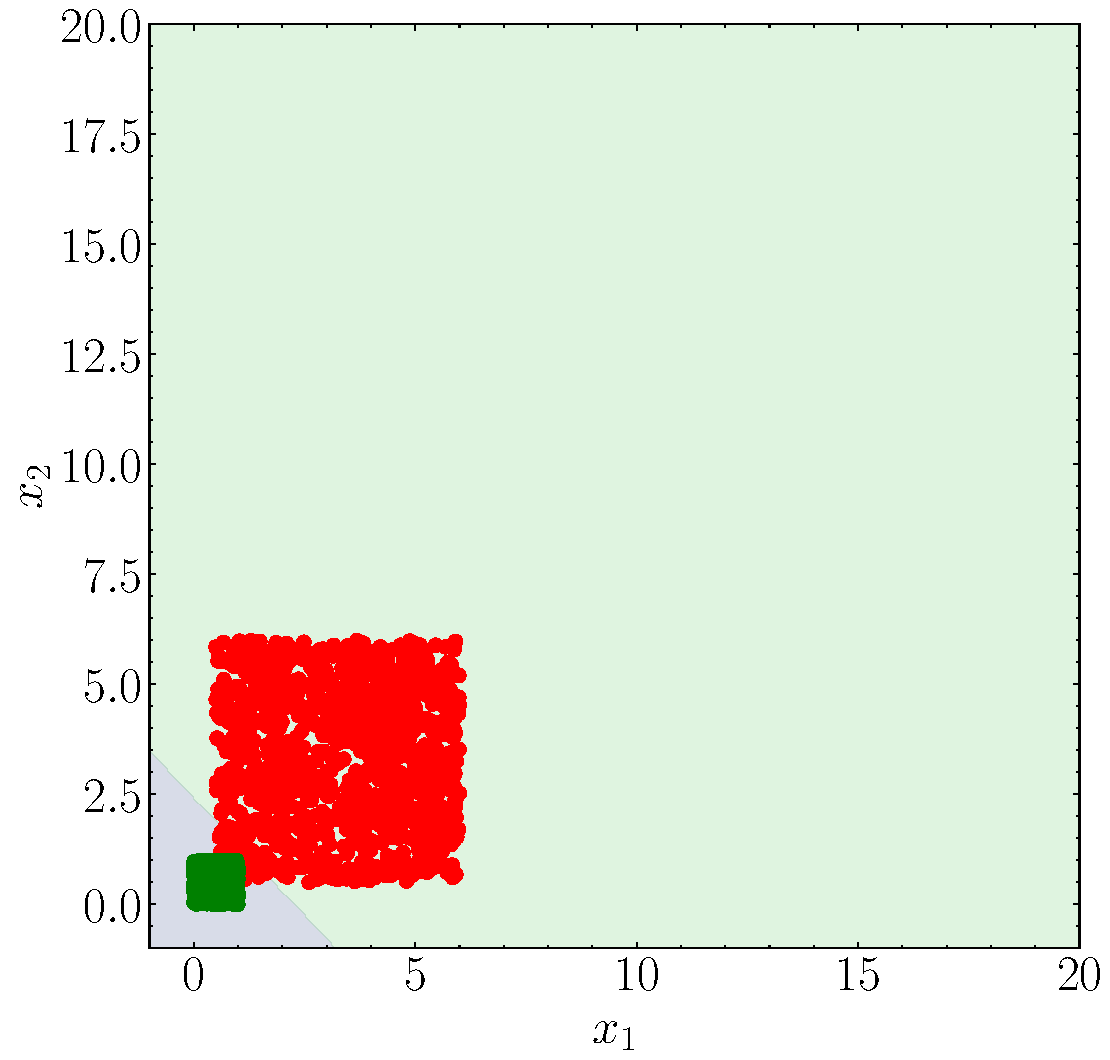
\includegraphics[width=1.5in]{../results/ex1/samples_LOG_dataset_Uniform_size_50}}

\subfigure[LS, Size $100$]{\label{fig:a}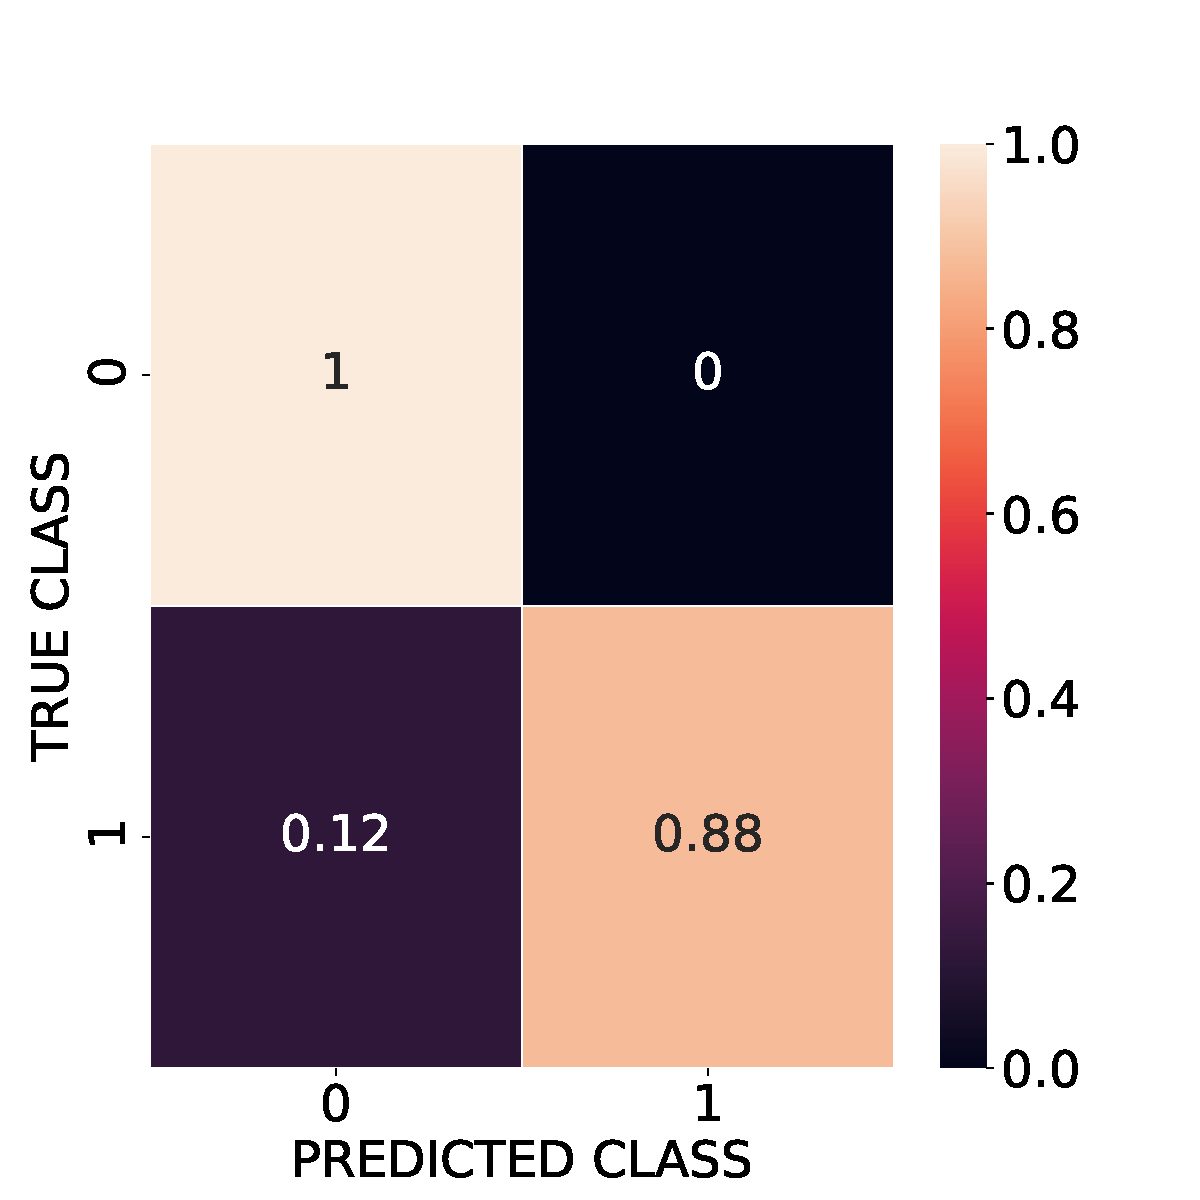
\includegraphics[width=1.5in]{../results/ex1/acc_LS_dataset_Uniform_size_100}}
\subfigure[LS Classifier]{\label{fig:a}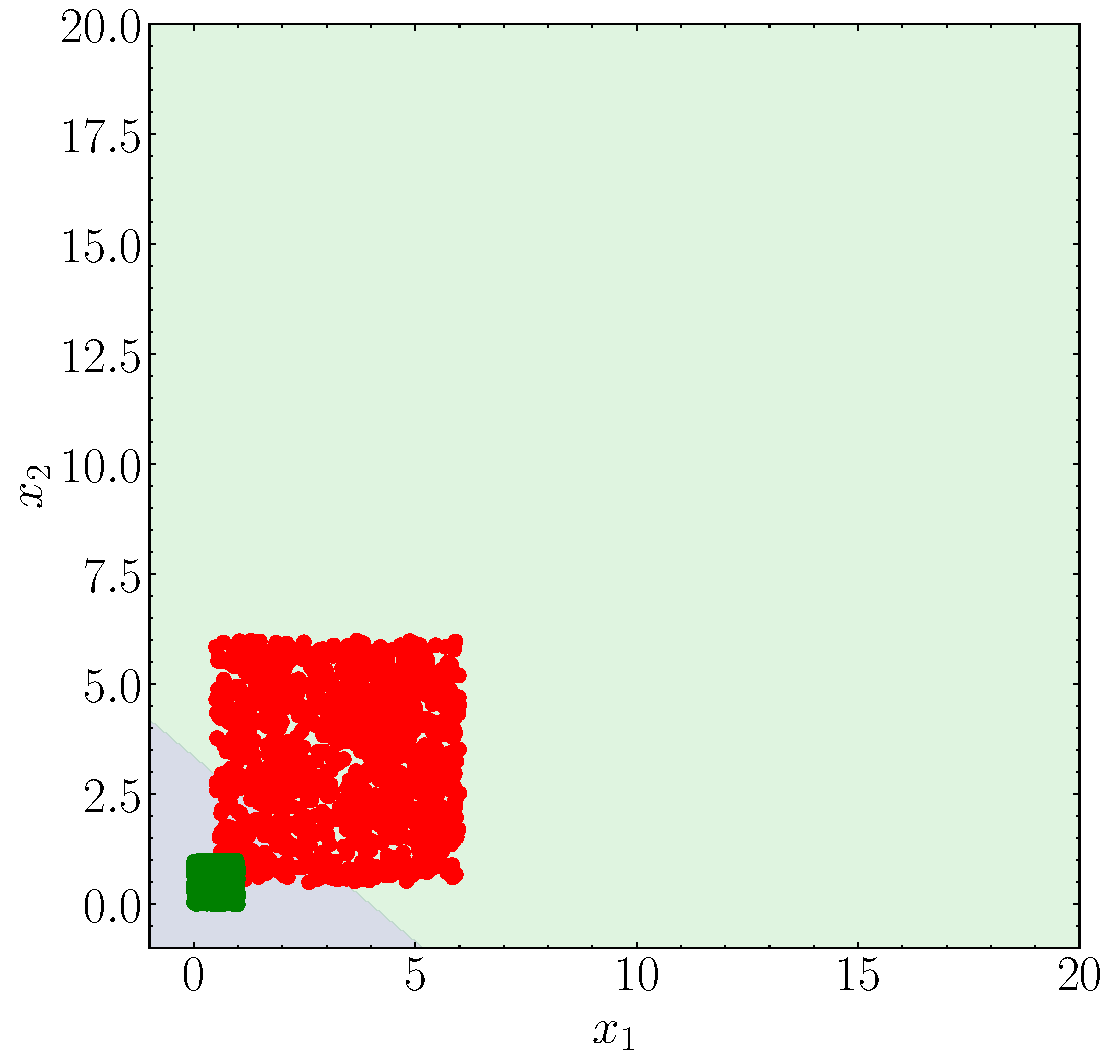
\includegraphics[width=1.5in]{../results/ex1/samples_LS_dataset_Uniform_size_100}}
\subfigure[LOG, Size $100$]{\label{fig:a}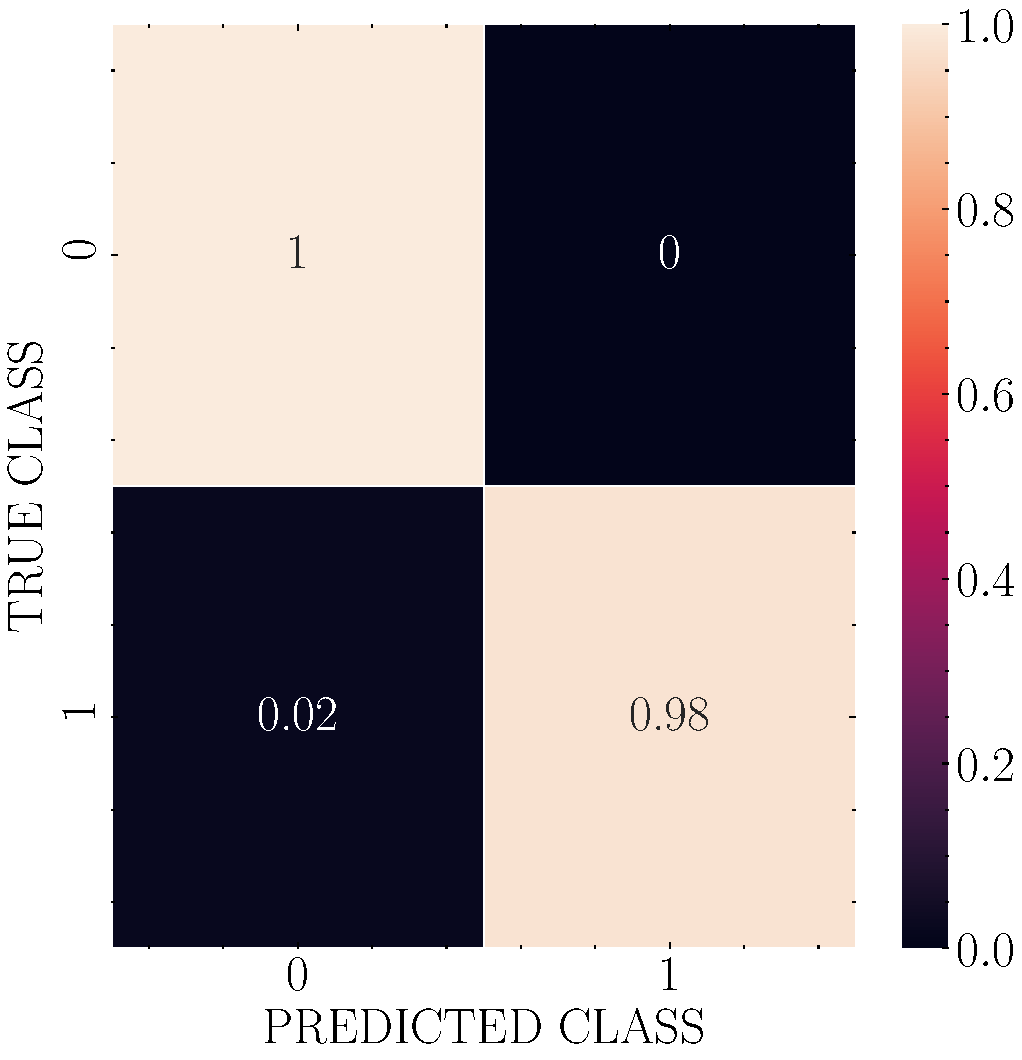
\includegraphics[width=1.5in]{../results/ex1/acc_LOG_dataset_Uniform_size_100}}
\subfigure[LOG Classifier]{\label{fig:a}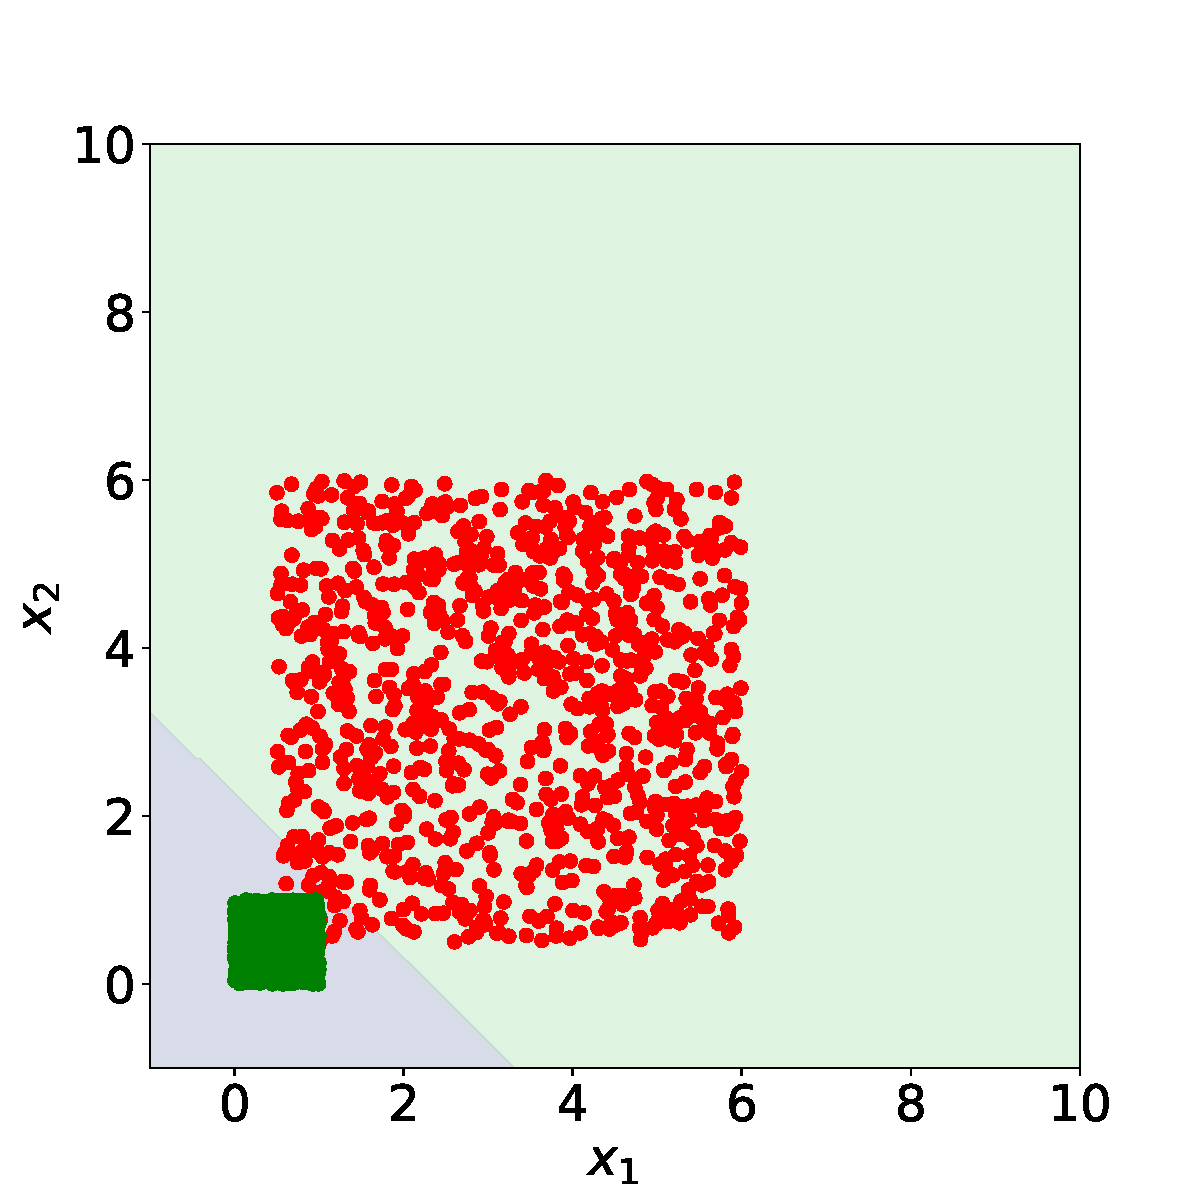
\includegraphics[width=1.5in]{../results/ex1/samples_LOG_dataset_Uniform_size_100}}

\subfigure[LS, Size $500$]{\label{fig:a}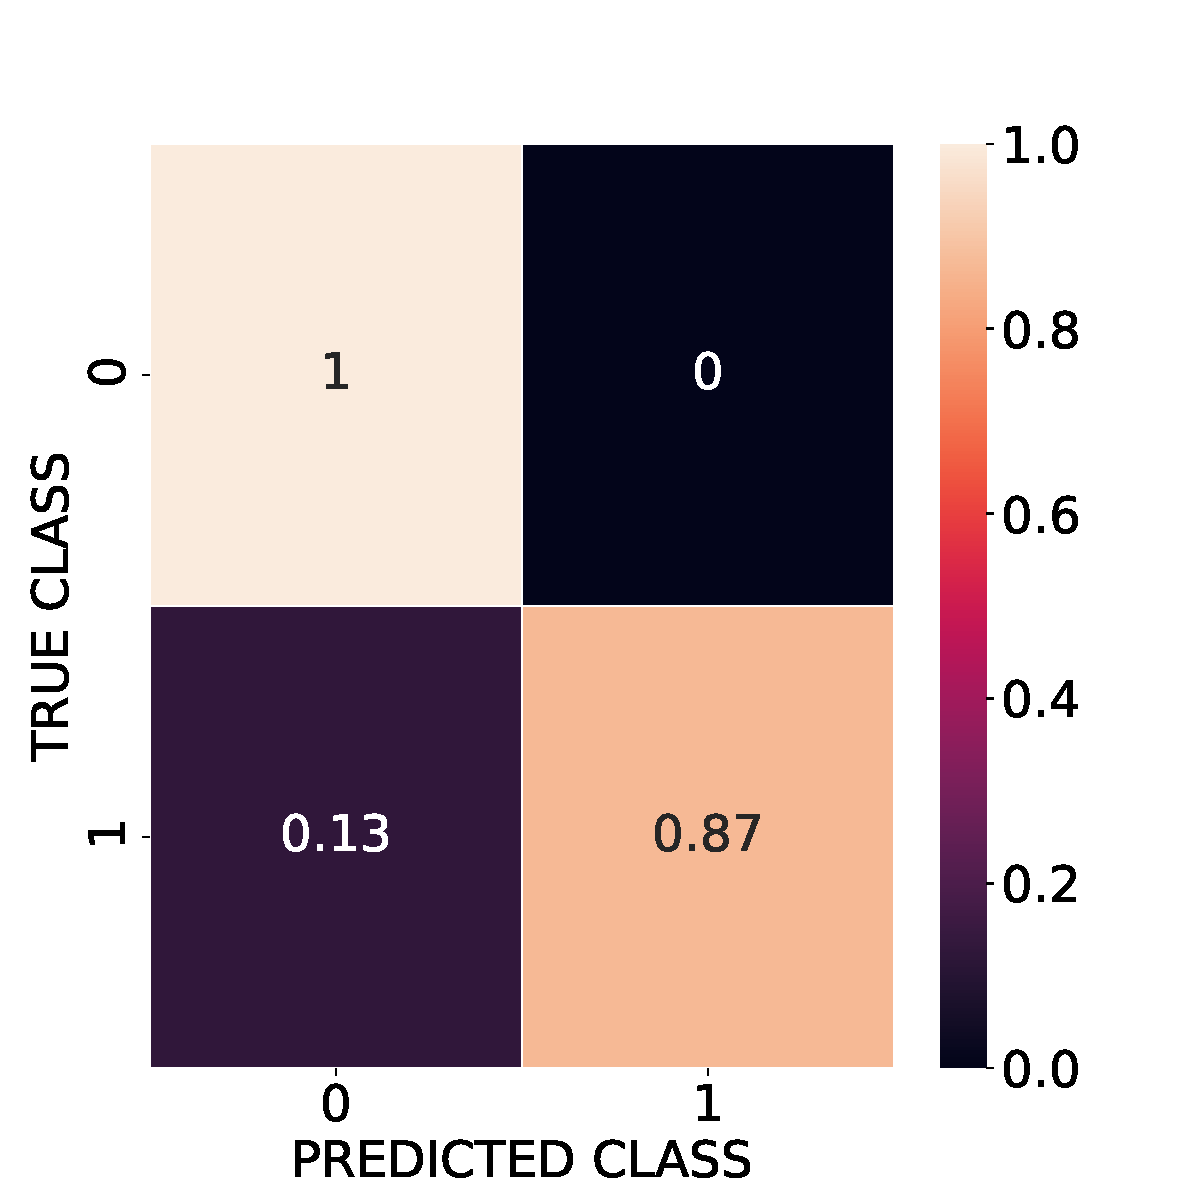
\includegraphics[width=1.5in]{../results/ex1/acc_LS_dataset_Uniform_size_500}}
\subfigure[LS Classifier]{\label{fig:a}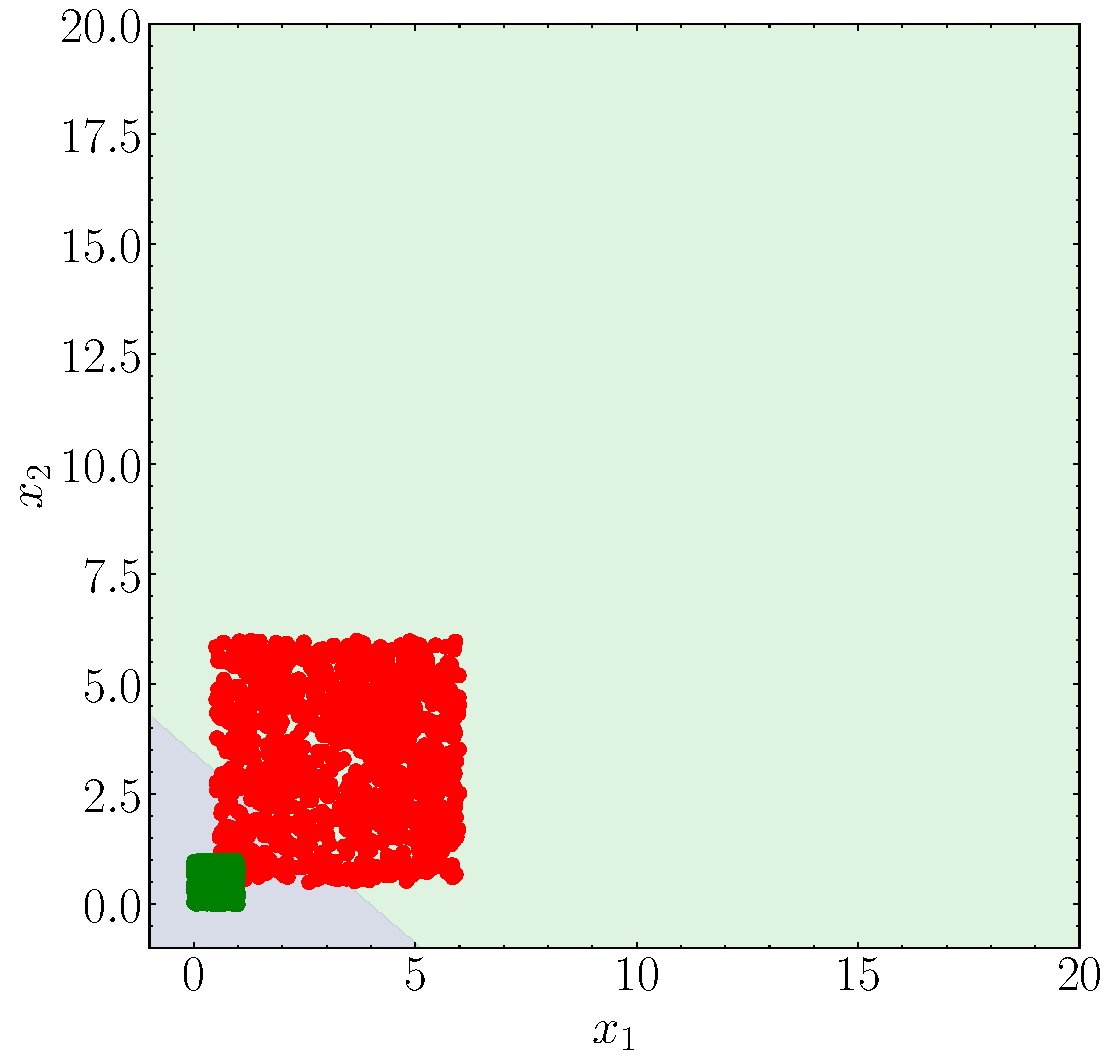
\includegraphics[width=1.5in]{../results/ex1/samples_LS_dataset_Uniform_size_500}}
\subfigure[LOG, Size $500$]{\label{fig:a}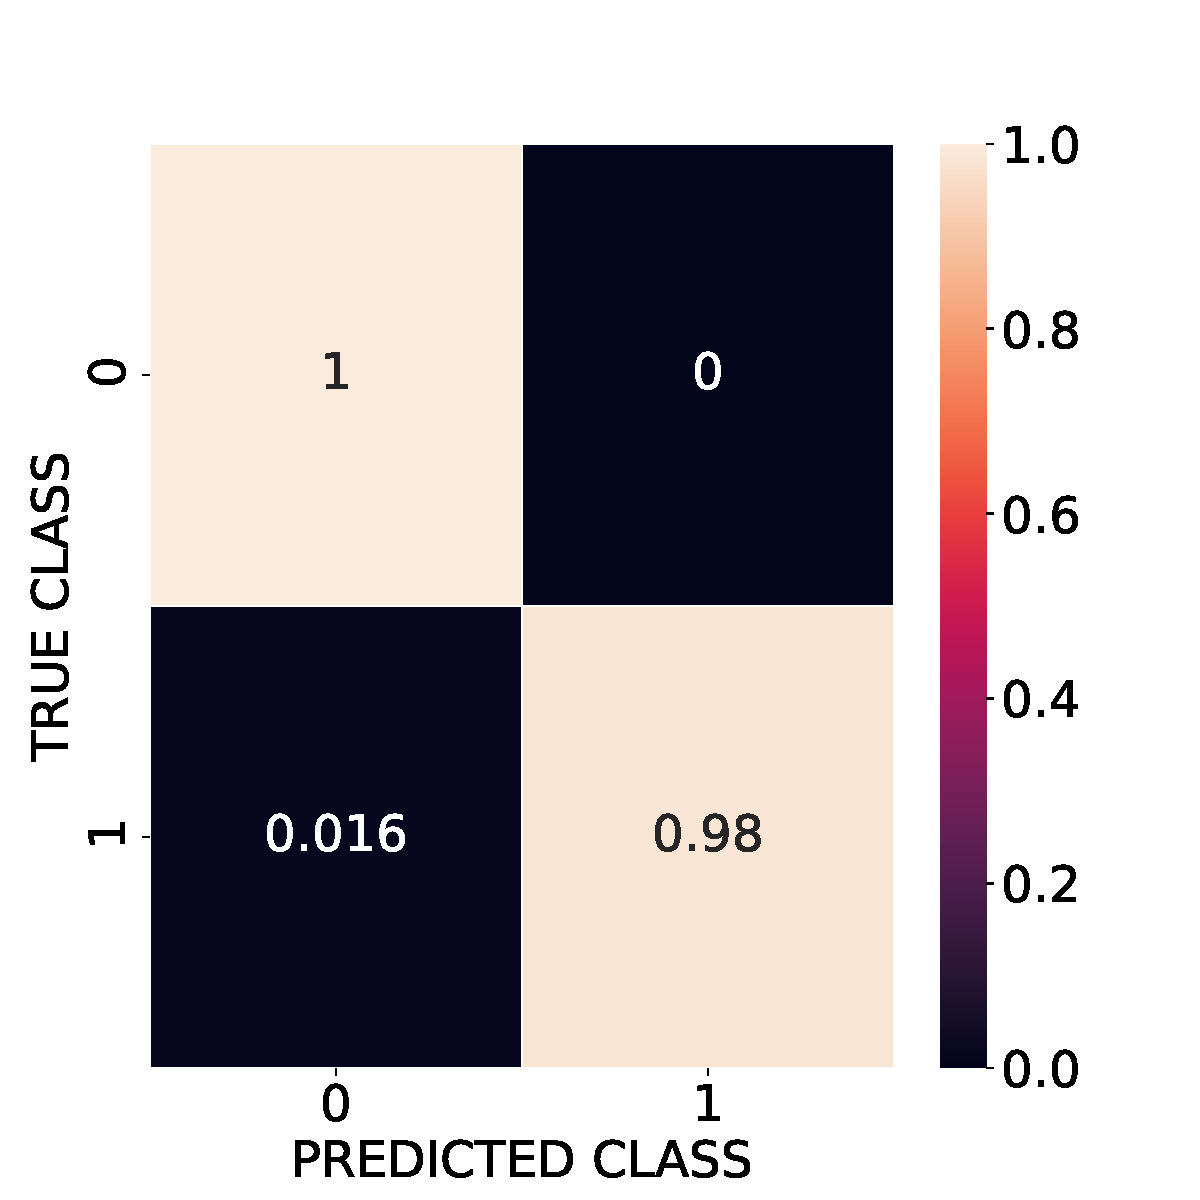
\includegraphics[width=1.5in]{../results/ex1/acc_LOG_dataset_Uniform_size_500}}
\subfigure[LOG Classifier]{\label{fig:a}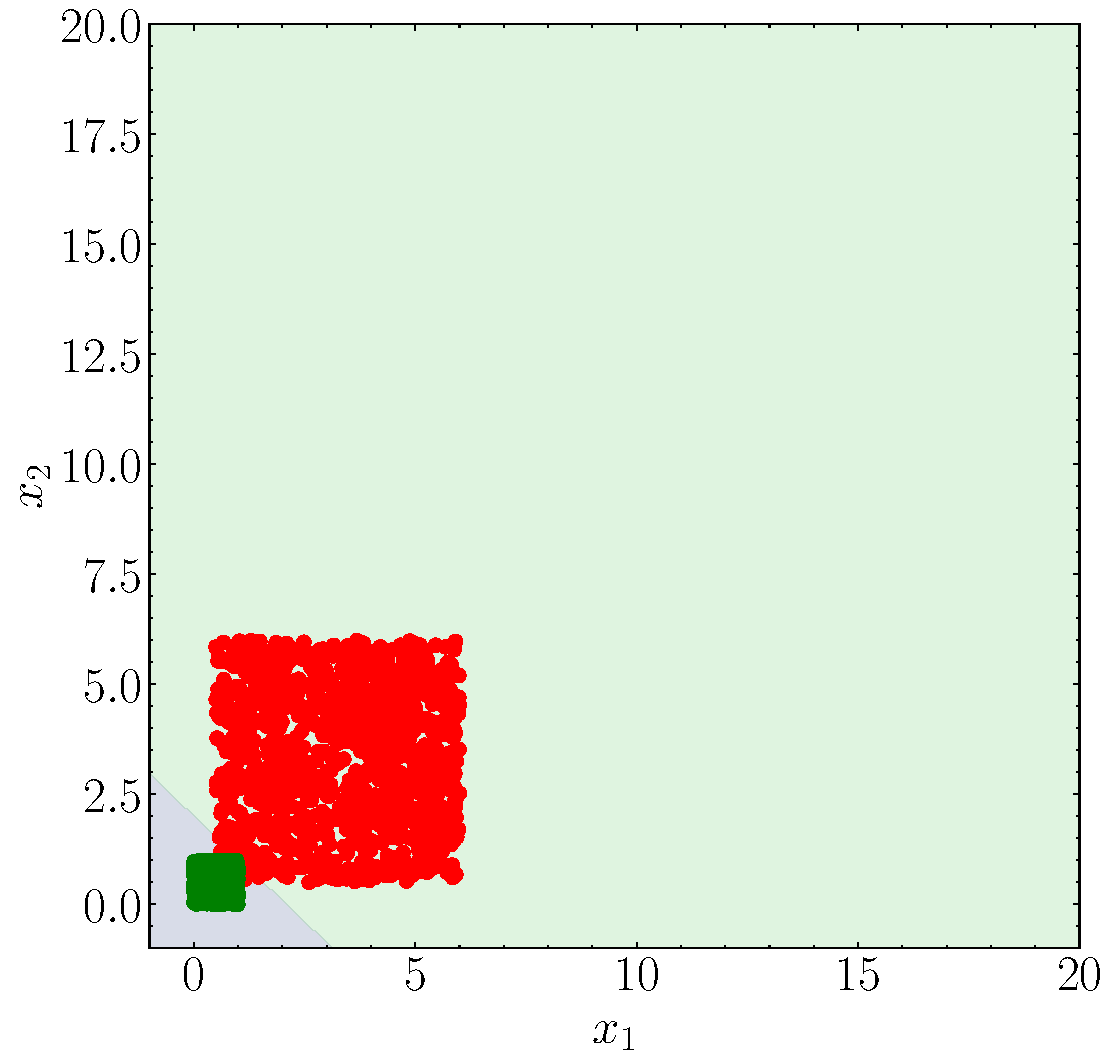
\includegraphics[width=1.5in]{../results/ex1/samples_LOG_dataset_Uniform_size_500}}

\subfigure[LS, Size $999$]{\label{fig:a}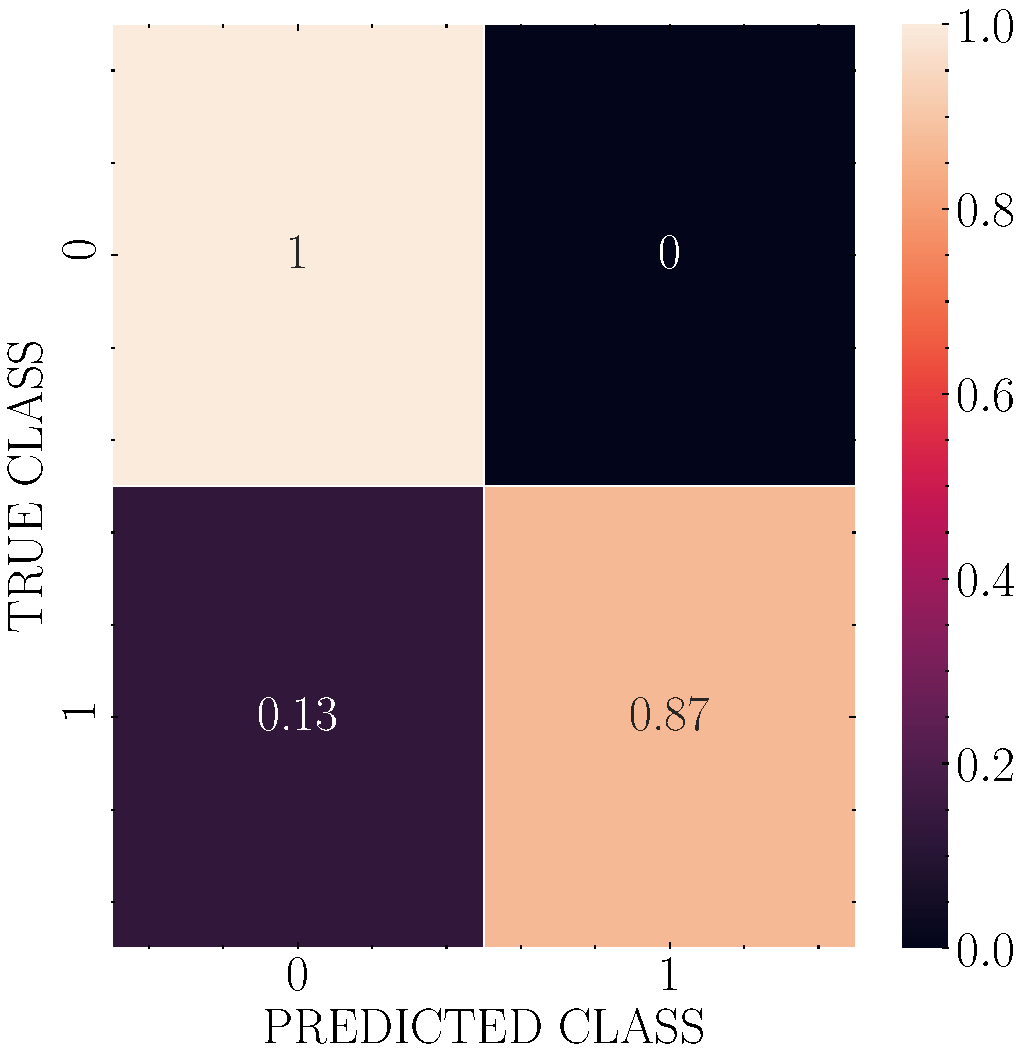
\includegraphics[width=1.5in]{../results/ex1/acc_LS_dataset_Uniform_size_999}}
\subfigure[LS Classifier]{\label{fig:a}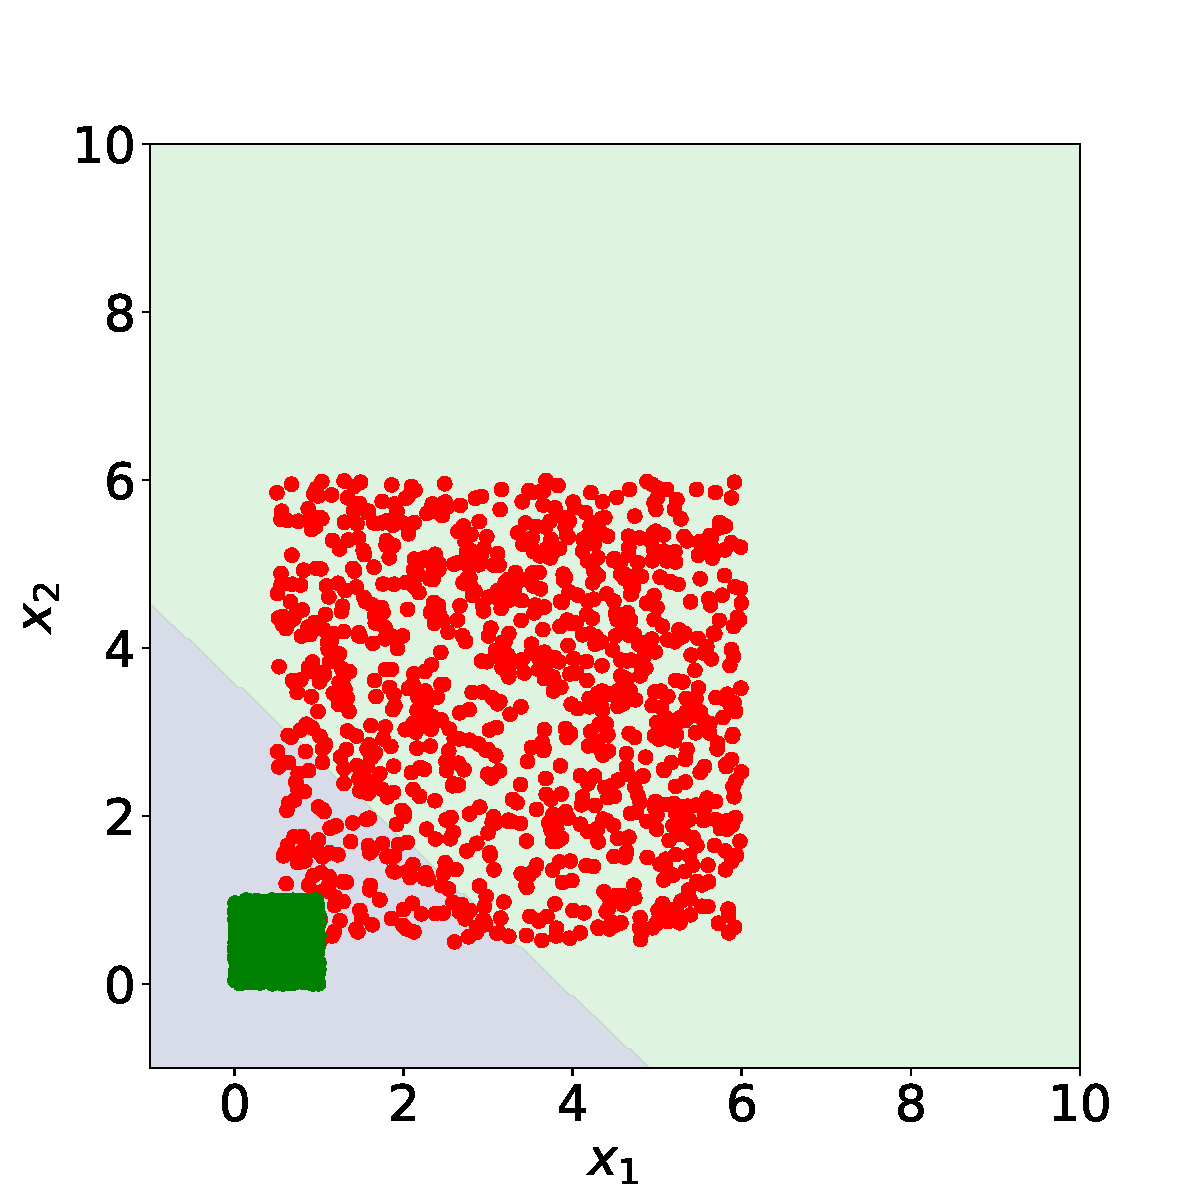
\includegraphics[width=1.5in]{../results/ex1/samples_LS_dataset_Uniform_size_999}}
\subfigure[LOG, Size $999$]{\label{fig:a}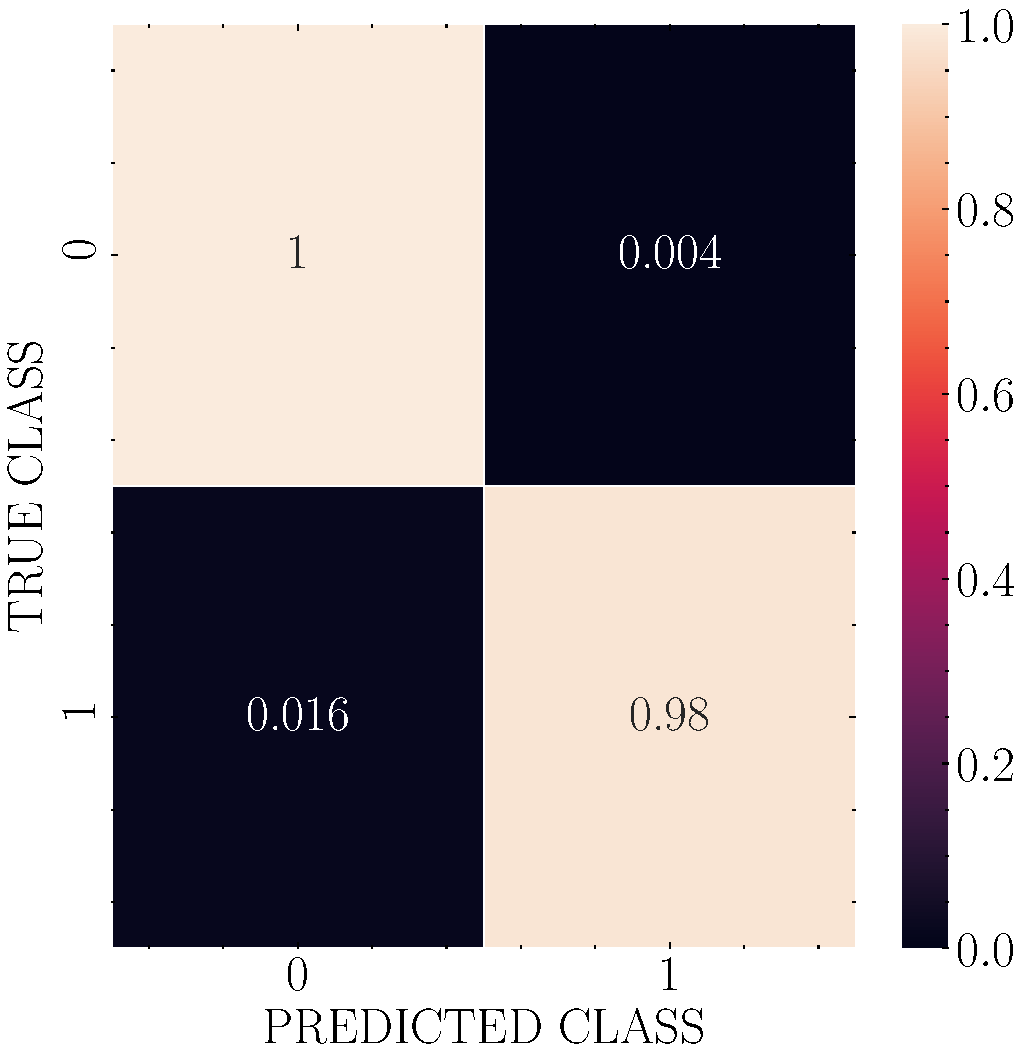
\includegraphics[width=1.5in]{../results/ex1/acc_LOG_dataset_Uniform_size_999}}
\subfigure[LOG Classifier]{\label{fig:a}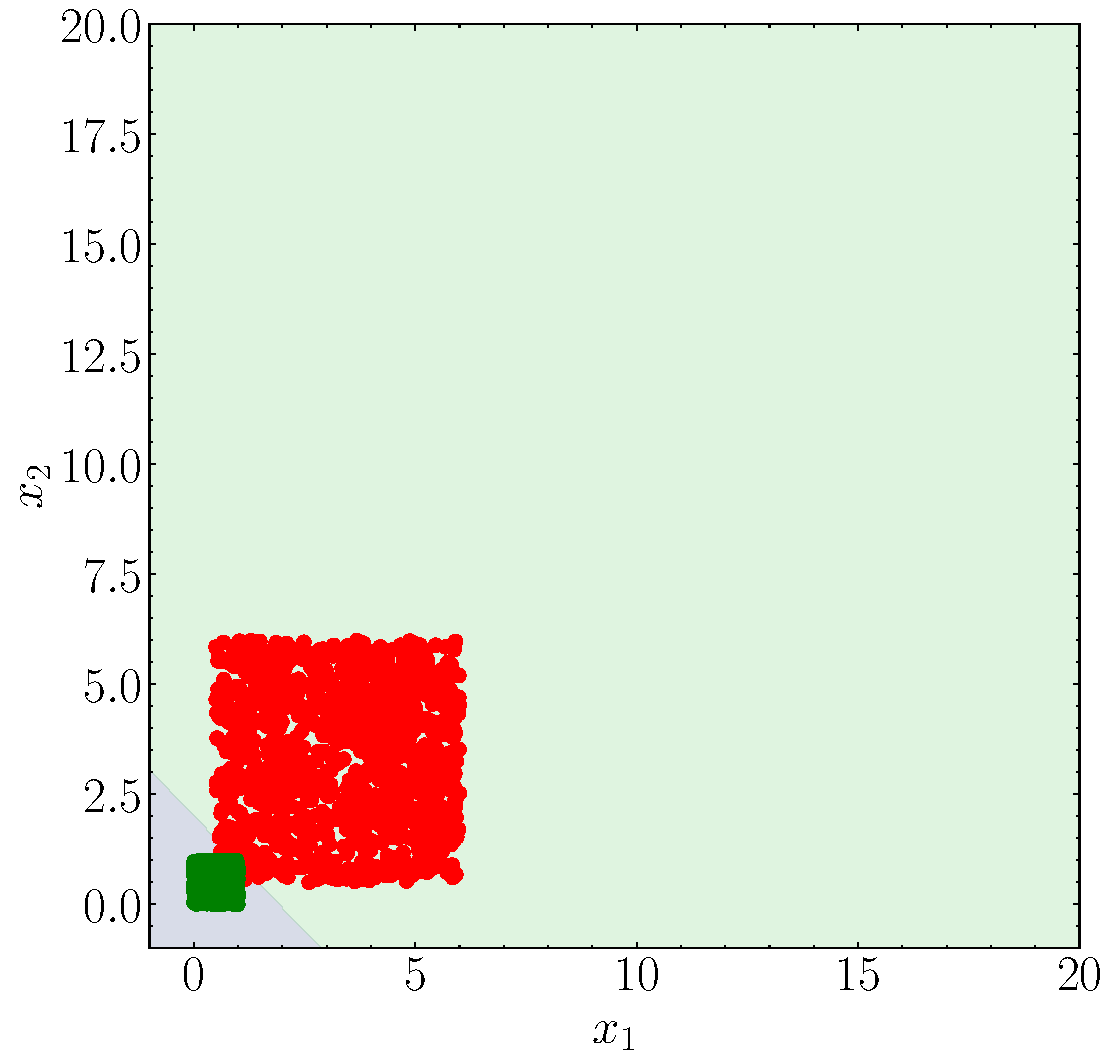
\includegraphics[width=1.5in]{../results/ex1/samples_LOG_dataset_Uniform_size_999}}

\caption{Linear Least-Squares Classifier and Logistic Regression on Uniform distributed data.}
\label{fig:LS_LOG_Uniform}
\end{figure}

{\it \bfseries Inferences:} It can be seen that the accuracy of the linear classifier does not vary with increasing training size. Since the least-squares cost equally penalises all points, class $0$ is always perfectly classified and the discriminant function always has a large offset owing to the larger spread of class $1$. In logistic regression, the accuracy increases with increasing training size. It is known that the Bayes' classifier for such class conditionals passes through the points of intersection of the squares generated by the limits of the class conditionals. With increasing training size, logistic regression approximately achieves the Bayes' classifier. In this case, logistic regression outperforms linear least-squares classification. \\

% ------------------------------------------------------------------------------------------------------------------------------------------------------

\problem{Problem (1.c) Gaussian-distributed Classes in 10D}
\label{prob:1.c}

Let the class conditionals be modelled as Gaussian distributions with different mean and identity covariance. The $2$-class linear least-squares (LS) classifier is trained by minimising (\ref{eq:lsClassifier}) and logistic regression (LOG) is trained using gradient descent with constant step-size using (\ref{eq:logGD}). \\

{\it \bfseries Results:} Figure \ref{fig:LS_LOG_Gaussian} shows the accuracies of classification in confusion matrices. The classifier and the training size used are mentioned in the respective captions. The accuracies reported are averaged over $10000$ realisations. \\

\begin{figure}
\centering
\subfigure[LS, Size $10$]{\label{fig:a}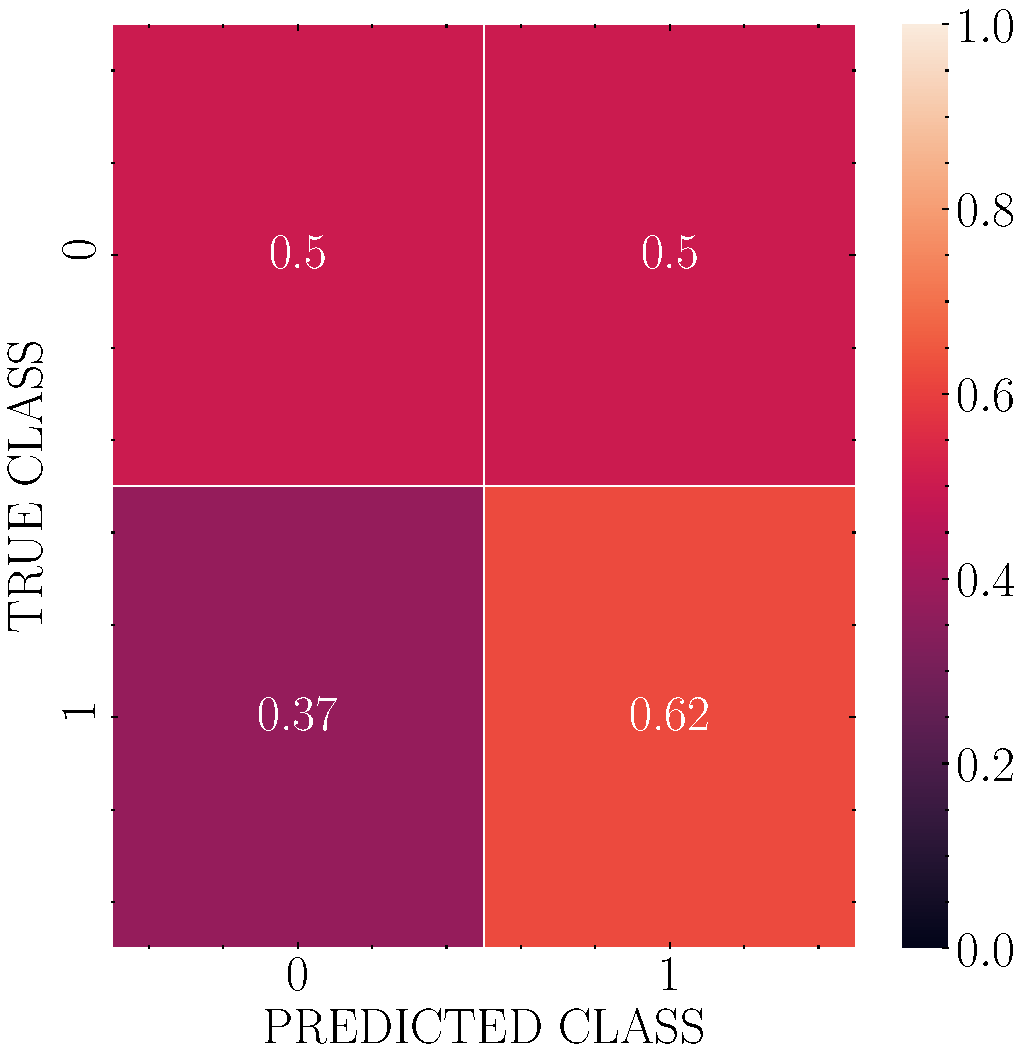
\includegraphics[width=1.5in]{../results/ex1/acc_LS_dataset_Normal_size_10}}
\subfigure[LOG, Size $10$]{\label{fig:a}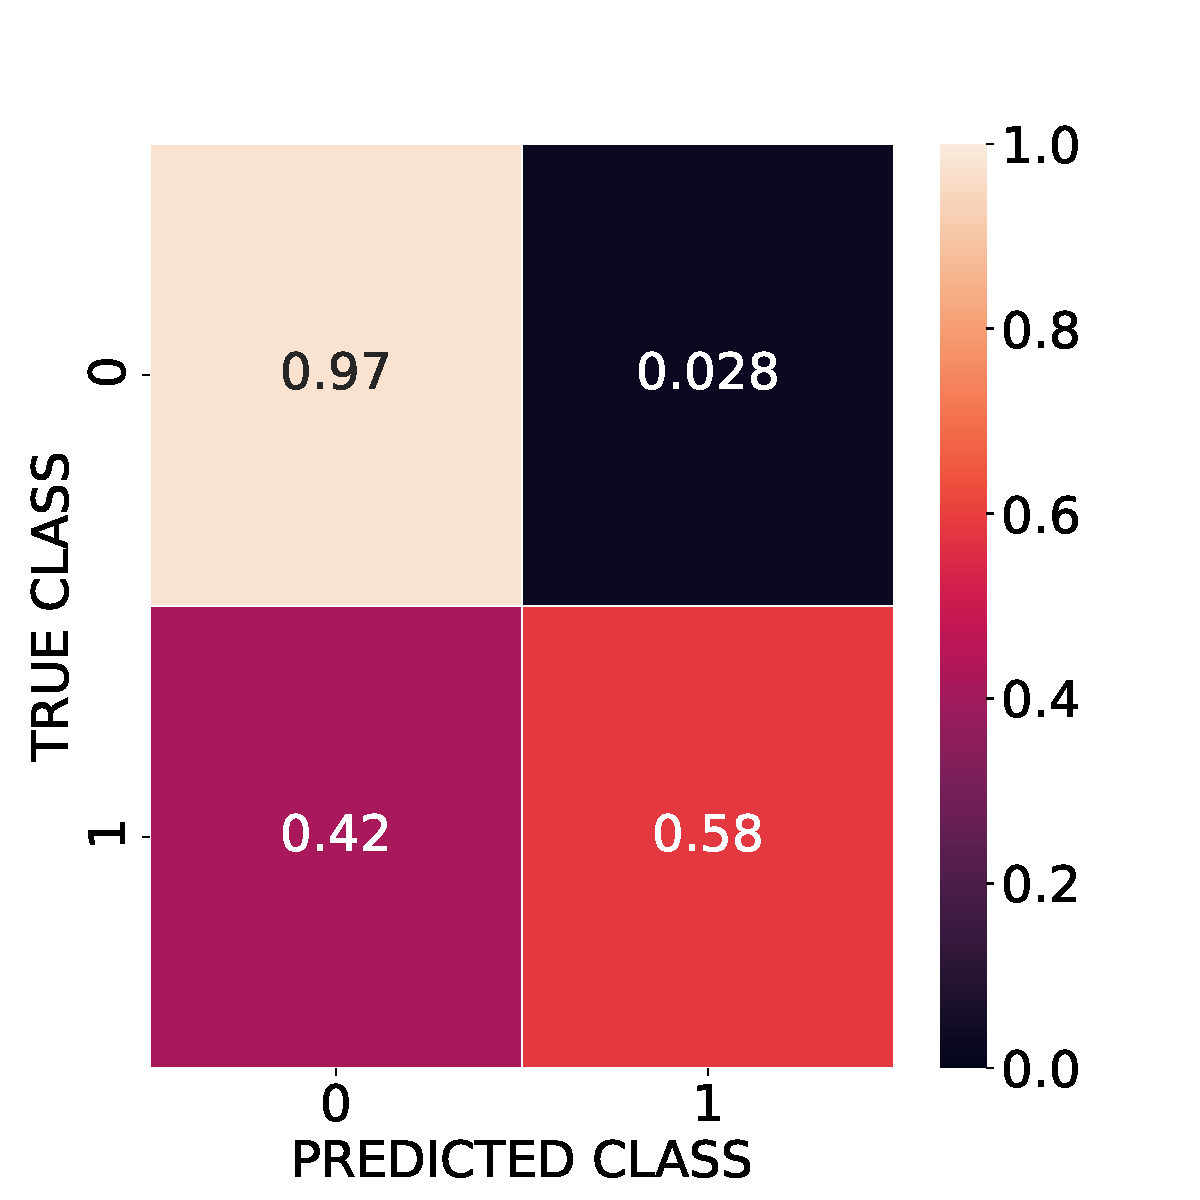
\includegraphics[width=1.5in]{../results/ex1/acc_LOG_dataset_Normal_size_10}}
\subfigure[LS, Size $50$]{\label{fig:a}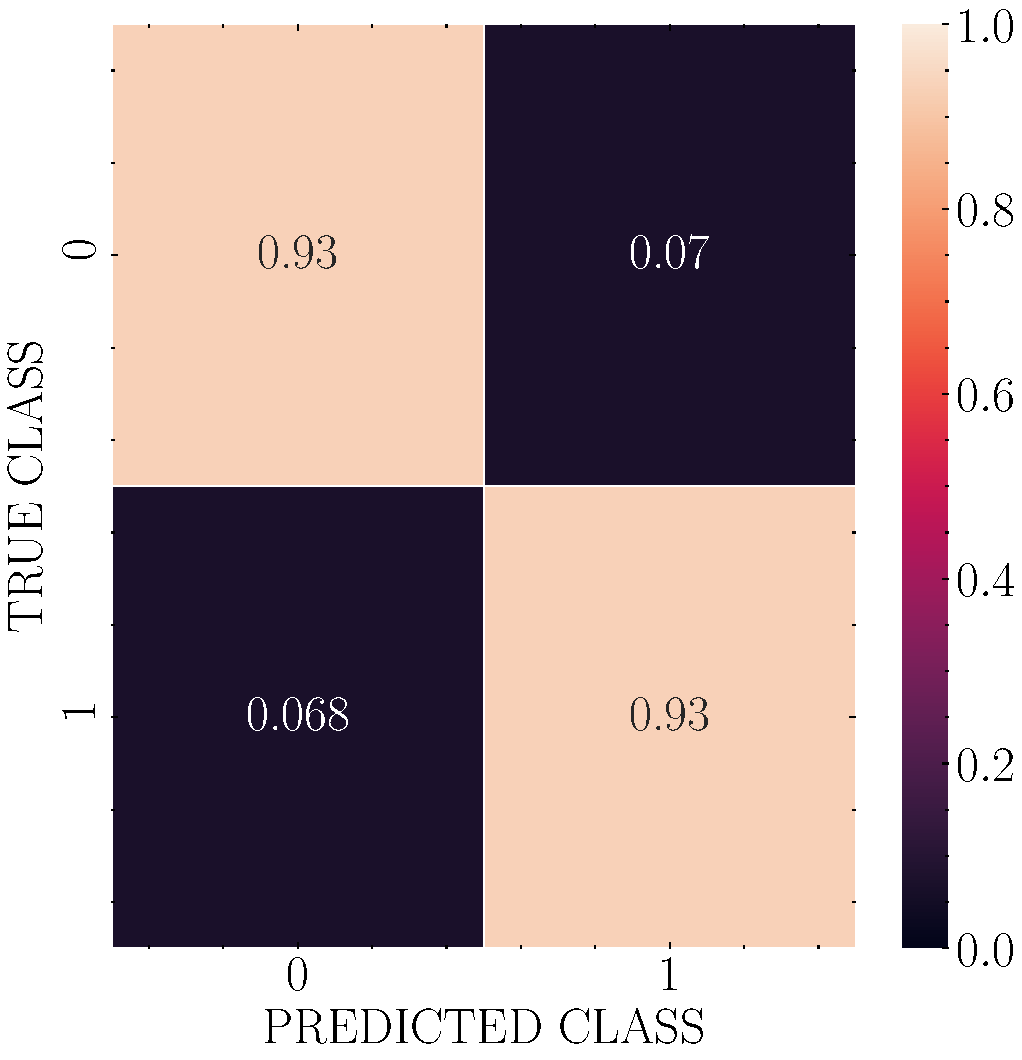
\includegraphics[width=1.5in]{../results/ex1/acc_LS_dataset_Normal_size_50}}
\subfigure[LOG, Size $50$]{\label{fig:a}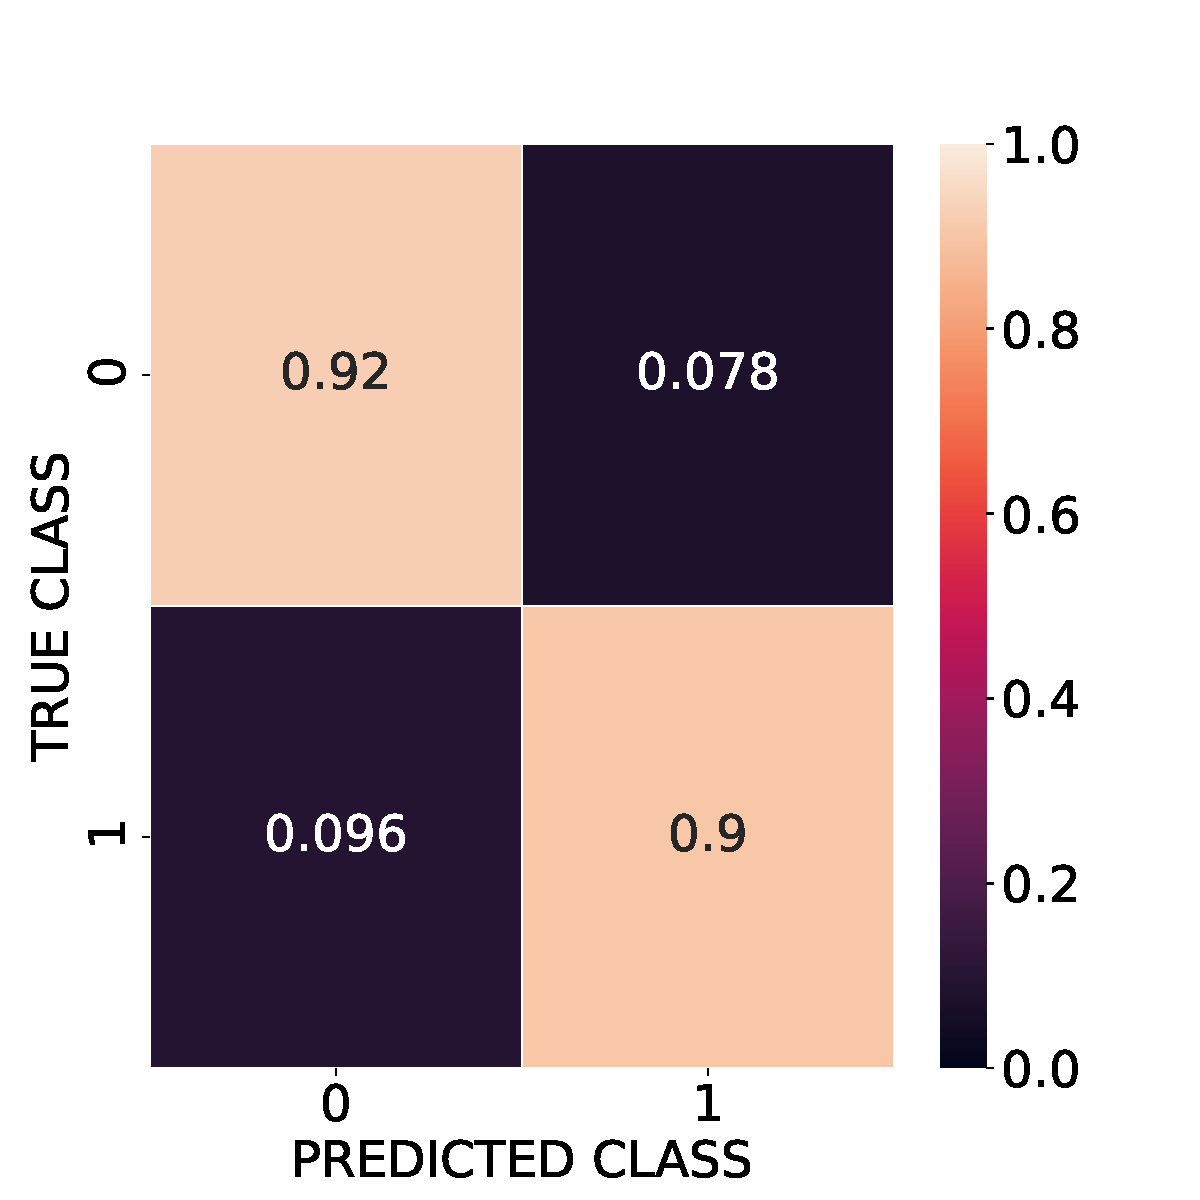
\includegraphics[width=1.5in]{../results/ex1/acc_LOG_dataset_Normal_size_50}}

\subfigure[LS, Size $100$]{\label{fig:a}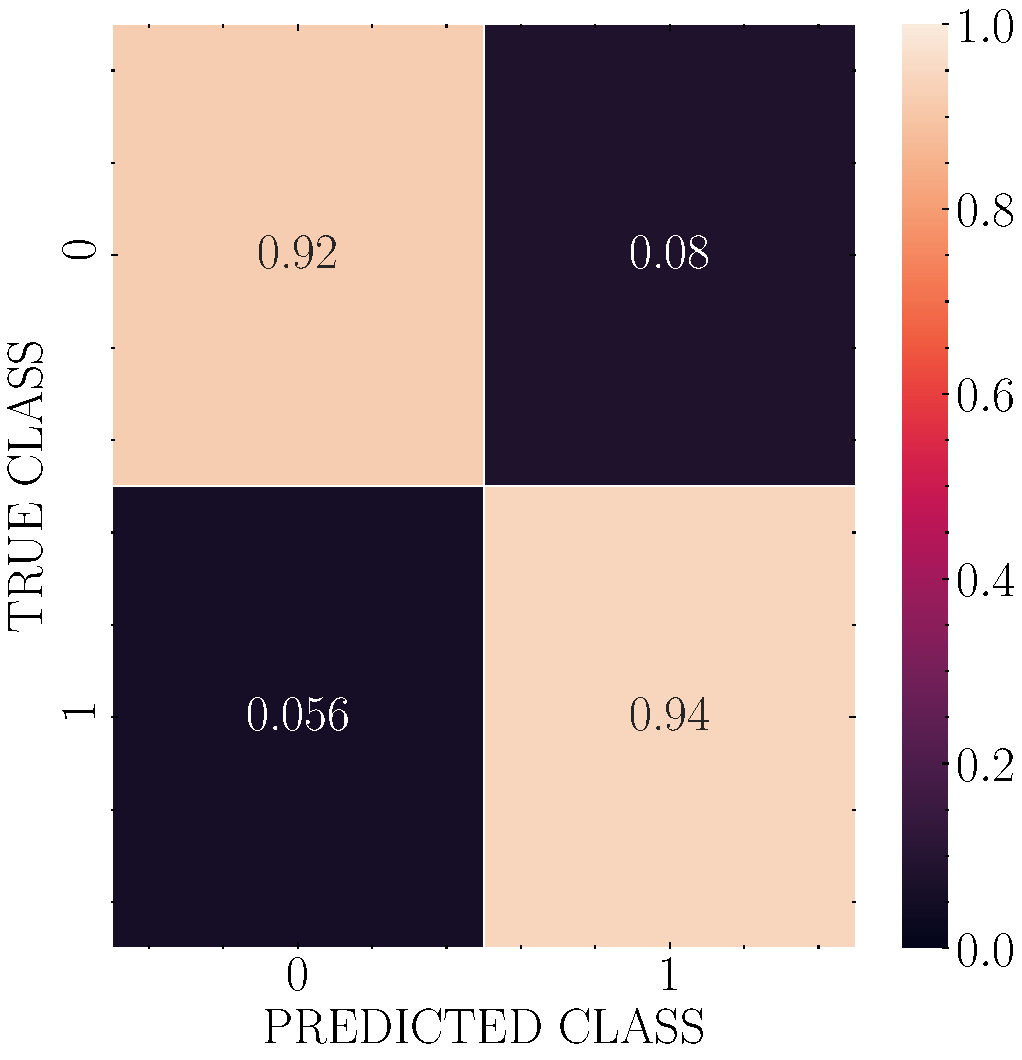
\includegraphics[width=1.5in]{../results/ex1/acc_LS_dataset_Normal_size_100}}
\subfigure[LOG, Size $100$]{\label{fig:a}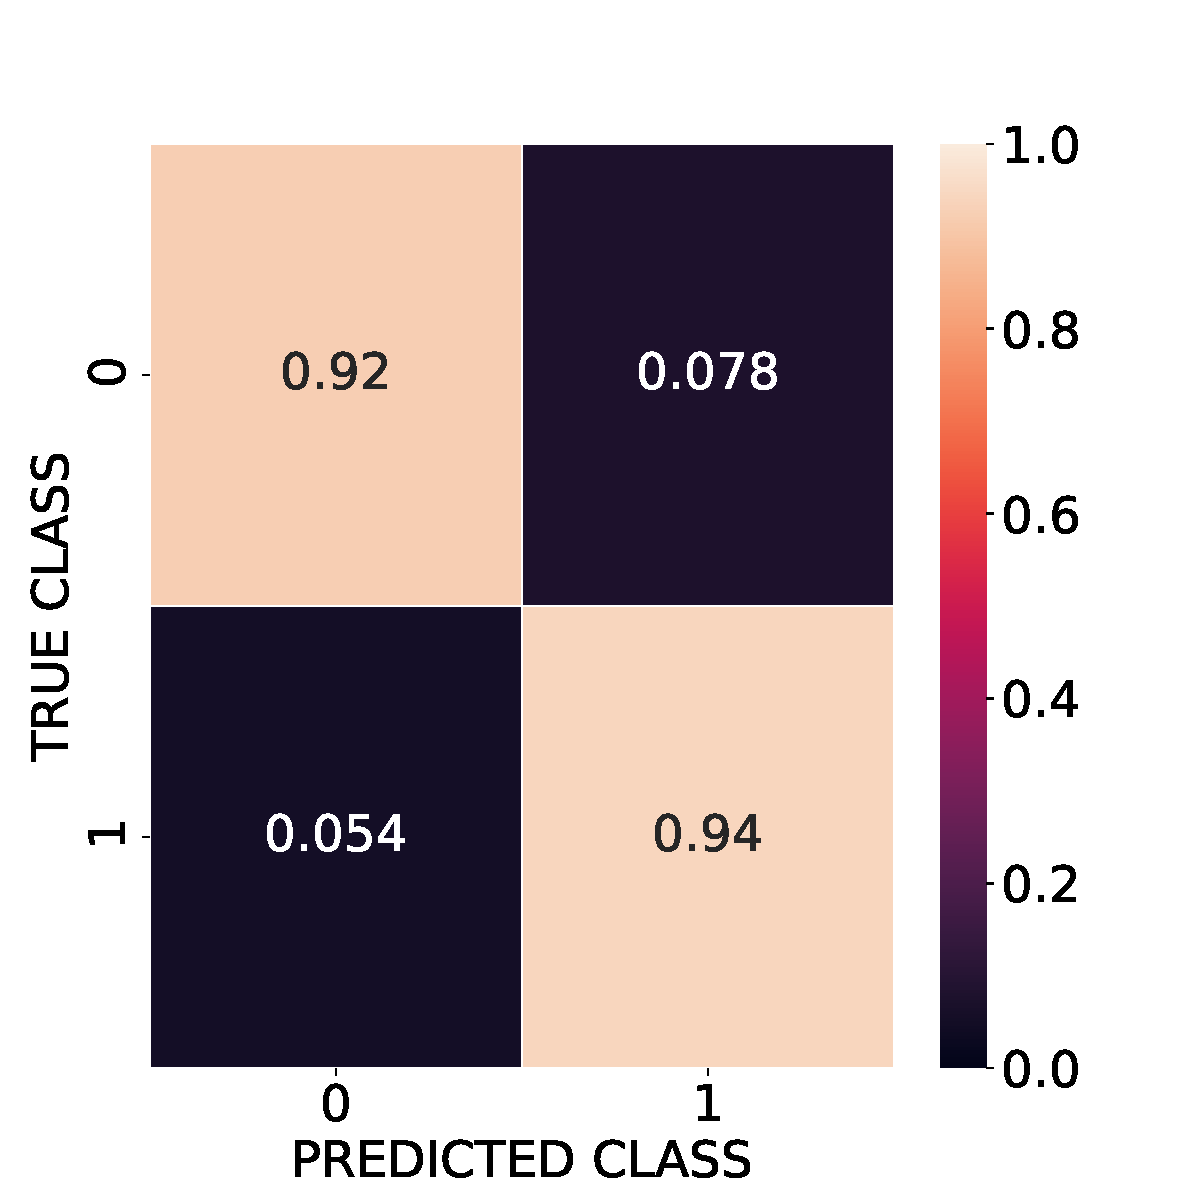
\includegraphics[width=1.5in]{../results/ex1/acc_LOG_dataset_Normal_size_100}}
\subfigure[LS, Size $500$]{\label{fig:a}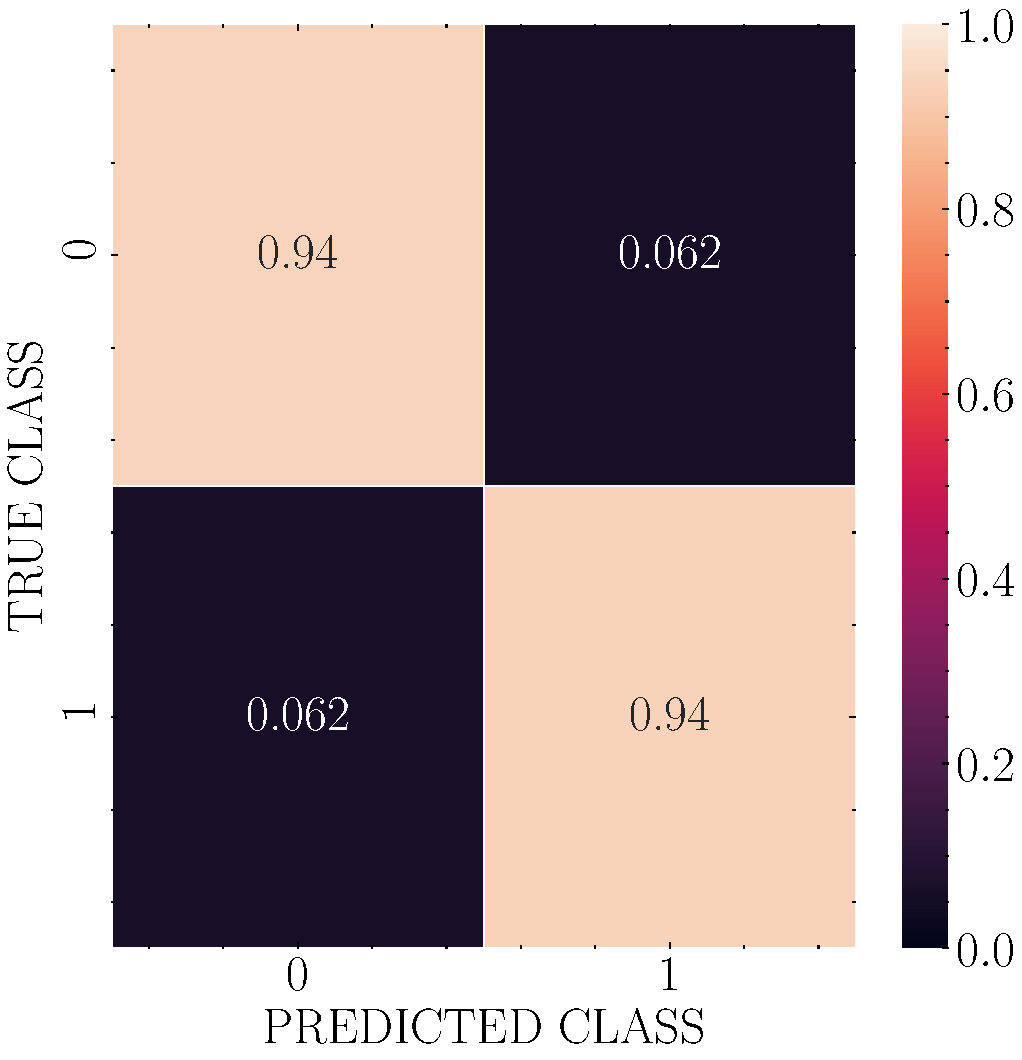
\includegraphics[width=1.5in]{../results/ex1/acc_LS_dataset_Normal_size_500}}
\subfigure[LOG, Size $500$]{\label{fig:a}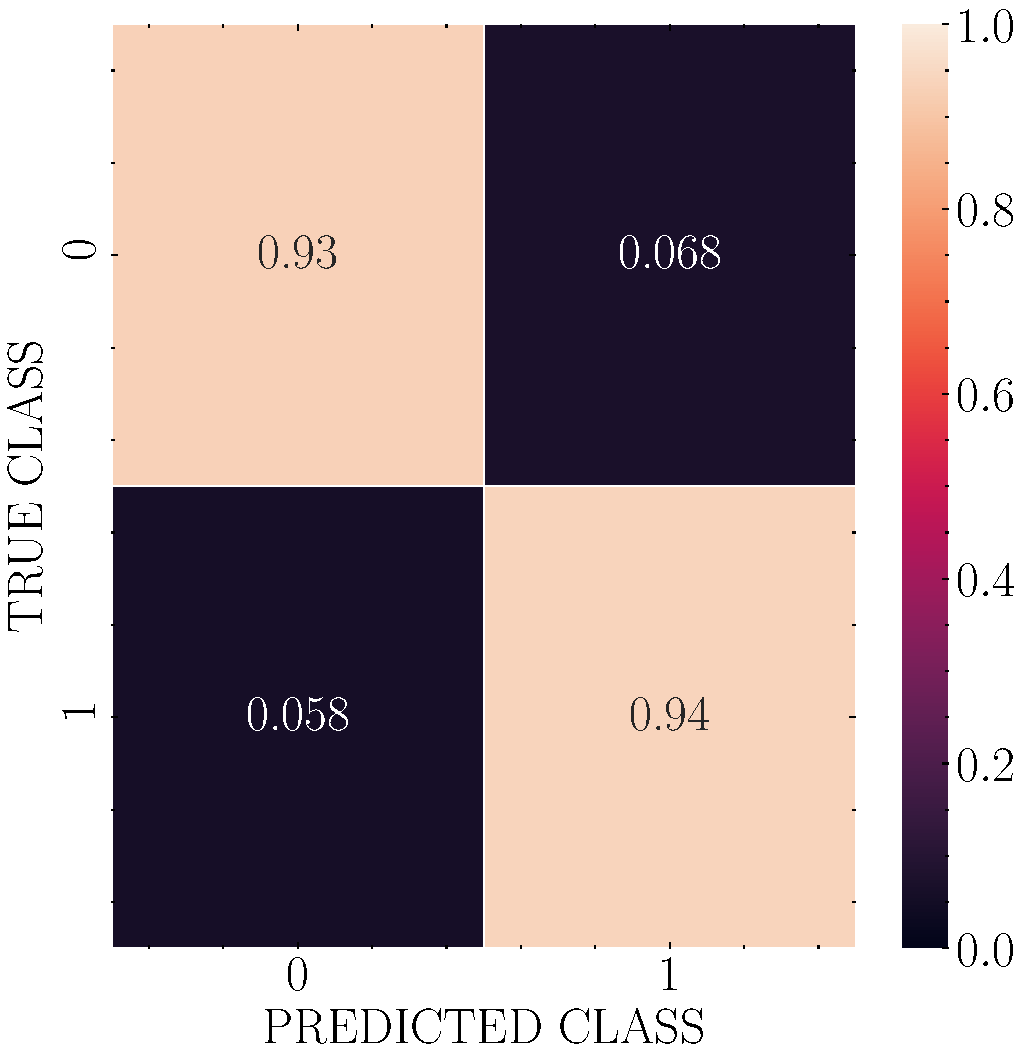
\includegraphics[width=1.5in]{../results/ex1/acc_LOG_dataset_Normal_size_500}}

\subfigure[LS, Size $999$]{\label{fig:a}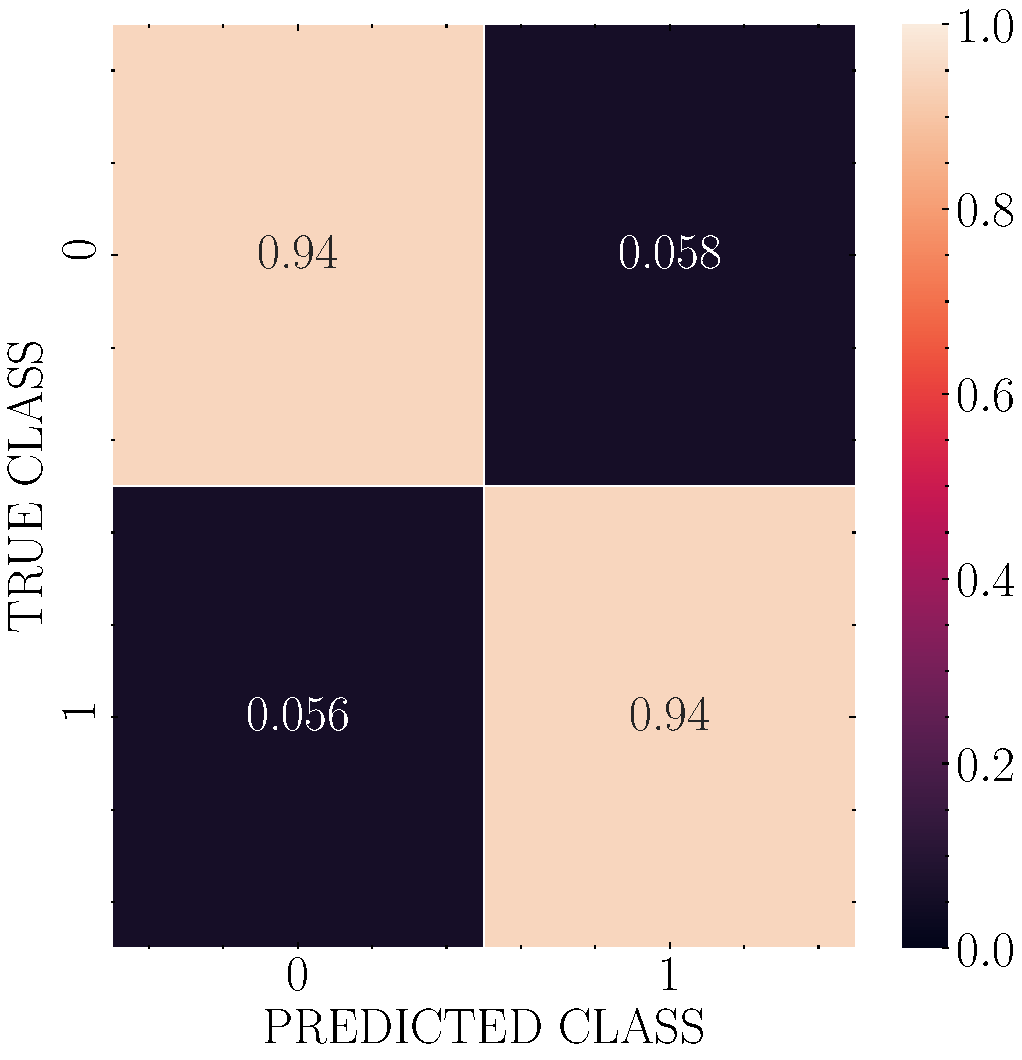
\includegraphics[width=1.5in]{../results/ex1/acc_LS_dataset_Normal_size_999}}
\subfigure[LOG, Size $999$]{\label{fig:a}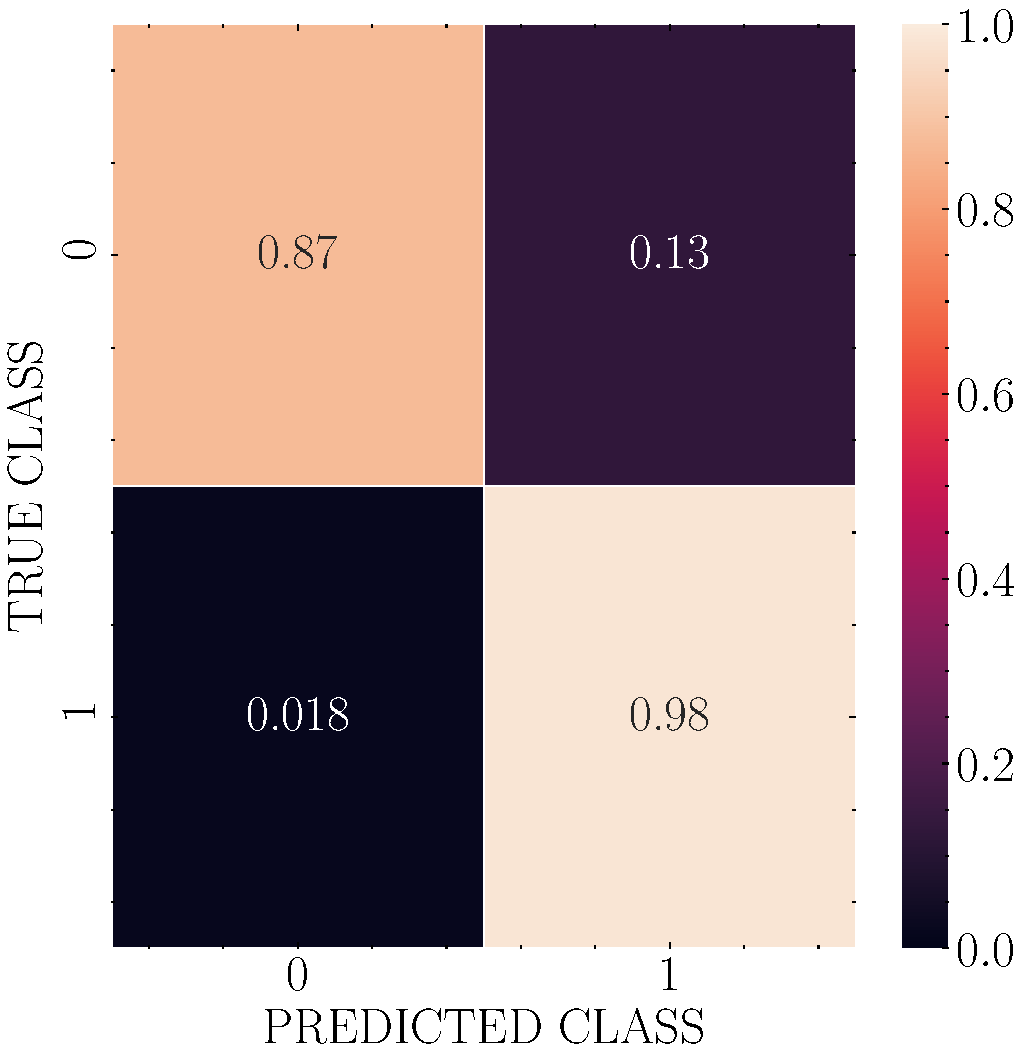
\includegraphics[width=1.5in]{../results/ex1/acc_LOG_dataset_Normal_size_999}}

\caption{Linear Least-Squares Classifier and Logistic Regression on Gaussian distributed data.}
\label{fig:LS_LOG_Gaussian}
\end{figure}

{\it \bfseries Inferences:} It can be seen that the accuracy of both the classifiers increase to the similar values. Since the class conditionals are Gaussian and have identity covariance, the linear least-squares classifier and logistic regression give approximately the same discriminant function. \\

% ------------------------------------------------------------------------------------------------------------------------------------------------------
% ------------------------------------------------------------------------------------------------------------------------------------------------------

\section{Multi-Class Linear Classification on Iris Dataset}
\label{sec:bayes20D}

The \texttt{iris} data set contains features in $\rr^{5}$ and classifies into three classes -- Iris Sentosa, Iris Versicolour and Iris Virginica.

\problem{Problem (2.i) One vs. Rest Classifier}
\label{prob:2.i}

In the one vs. rest mode, three binary classifiers are learnt as Iris Sentosa vs. not Iris Sentosa, Iris Versicolour and not Iris Versicolour and Iris Virginica and not Iris Virginica. In this mode of multi-class classification, ambiguities may arise when multiple class flag the feature into the true class. The linear least-squares classifier are trained by minimising (\ref{eq:lsClassifier}). \\

{\it \bfseries Results:} Figure \ref{fig:LSOA_Iris} shows the confusion matrices for each class with varying train-test split fraction of the dataset. The resultant accuracies are shown in the respective titles. The results are averaged over $10000$ realisations. \\

\begin{figure}
\centering
\subfigure[Class $0$, Fraction $0.2$]{\label{fig:a}\includegraphics[width=1.5in]{../results/ex2/acc_LSOA_dataset_iris_fraction_0.2_class_0}}
\subfigure[Class $1$, Fraction $0.2$]{\label{fig:a}\includegraphics[width=1.5in]{../results/ex2/acc_LSOA_dataset_iris_fraction_0.2_class_1}}
\subfigure[Class $2$, Fraction $0.2$]{\label{fig:a}\includegraphics[width=1.5in]{../results/ex2/acc_LSOA_dataset_iris_fraction_0.2_class_2}}

\subfigure[Class $0$, Fraction $0.4$]{\label{fig:a}\includegraphics[width=1.5in]{../results/ex2/acc_LSOA_dataset_iris_fraction_0.4_class_0}}
\subfigure[Class $1$, Fraction $0.4$]{\label{fig:a}\includegraphics[width=1.5in]{../results/ex2/acc_LSOA_dataset_iris_fraction_0.4_class_1}}
\subfigure[Class $2$, Fraction $0.4$]{\label{fig:a}\includegraphics[width=1.5in]{../results/ex2/acc_LSOA_dataset_iris_fraction_0.4_class_2}}

\subfigure[Class $0$, Fraction $0.6$]{\label{fig:a}\includegraphics[width=1.5in]{../results/ex2/acc_LSOA_dataset_iris_fraction_0.6_class_0}}
\subfigure[Class $1$, Fraction $0.6$]{\label{fig:a}\includegraphics[width=1.5in]{../results/ex2/acc_LSOA_dataset_iris_fraction_0.6_class_1}}
\subfigure[Class $2$, Fraction $0.6$]{\label{fig:a}\includegraphics[width=1.5in]{../results/ex2/acc_LSOA_dataset_iris_fraction_0.6_class_2}}

\subfigure[Class $0$, Fraction $0.8$]{\label{fig:a}\includegraphics[width=1.5in]{../results/ex2/acc_LSOA_dataset_iris_fraction_0.8_class_0}}
\subfigure[Class $1$, Fraction $0.8$]{\label{fig:a}\includegraphics[width=1.5in]{../results/ex2/acc_LSOA_dataset_iris_fraction_0.8_class_1}}
\subfigure[Class $2$, Fraction $0.8$]{\label{fig:a}\includegraphics[width=1.5in]{../results/ex2/acc_LSOA_dataset_iris_fraction_0.8_class_2}}

\caption{One vs. Rest Linear Least-Squares Classifier with varying train-test split fraction.}
\label{fig:LSOA_Iris}
\end{figure}

{\it \bfseries Inference:} In general, it can be seen that the accuracy of classification increases in each class with increasing test size. However, this does not give any information to resolve ambiguities. The scores corresponding to each class are lost, and three decisions are obtained. Such multi-class classification is useful when the decision at interest is to know if the class is Iris Sentosa vs. not Iris Sentosa, or so on and the decision of Iris Versicolour and Iris Viriginica are irrelevant.

% ------------------------------------------------------------------------------------------------------------------------------------------------------

\problem{Problem (2.ii) Multiclass Classifier}
\label{prob:2.ii}

In the multi-class mode, one $3$-class classifier using the method described in Section \ref{subsec:linearRegression}, by considering labels to be corresponding one-hot vectors to learn a score function that scores classification for each class. In this mode, there is no ambiguity in classifying a new feature in to one of the three classes, as there is always a unique class that provides the highest score (ties maybe resolved arbitrarily). However, this may come at a cost of reduced accuracy in classification. \\

{\it \bfseries Results:} Figure \ref{fig:LSMC_Iris} shows the confusion matrices for each class with varying train-test split fraction of the dataset. The resultant accuracies are shown in the respective titles. The results are averaged over $10000$ realisations. \\

\begin{figure}
\centering
\subfigure[Fraction $0.2$]{\label{fig:a}\includegraphics[width=1.5in]{../results/ex2/acc_LSMC_dataset_iris_fraction_0.2}}
\subfigure[Fraction $0.4$]{\label{fig:a}\includegraphics[width=1.5in]{../results/ex2/acc_LSMC_dataset_iris_fraction_0.4}}
\subfigure[Fraction $0.6$]{\label{fig:a}\includegraphics[width=1.5in]{../results/ex2/acc_LSMC_dataset_iris_fraction_0.6}}
\subfigure[Fraction $0.8$]{\label{fig:a}\includegraphics[width=1.5in]{../results/ex2/acc_LSMC_dataset_iris_fraction_0.8}}

\caption{Multi-class Linear Least-Squares Classifier with varying train-test split fraction.}
\label{fig:LSMC_Iris}
\end{figure}

{\it \bfseries Inference:} It can be seen that the accuracy of classification increases with increasing train-test split fraction. In such classification, the decision is not ambiguous -- the output for each new feature is a unique class label. However, as compared to accuracies in Figure \ref{fig:LSOA_Iris}, the accuracies are lower, i.e. an unambiguous decision is made with lesser confidence. Such multi-class classification is useful when the decision at interest is to know exactly which class the new feature belongs, where all classifications are relevant.

% ------------------------------------------------------------------------------------------------------------------------------------------------------
% ------------------------------------------------------------------------------------------------------------------------------------------------------

\section{Linear Classification on Financial Data}
\label{sec:german}

The \texttt{german.data-numeric} dataset contains features in $\rr^{24}$ related to finance of individuals and classifies into two classes -- bad and good. The data provided are in varying ranges, some are scores and some are binary flags. Hence, some data preprocessing maybe needed to obtain useful results. \\

{\it \bfseries Implementation:} Linear Least-Squares and Logistic Regression are used for classification. Two data preprocessing methods are considered -- normalisation and whitening. The linear least-squares classifier is trained by minimising (\ref{eq:lsClassifier}) and logistic regression (LOG) is trained using gradient descent with constant step-size using (\ref{eq:logGD}). \\

{\it \bfseries Results:} Figure \ref{fig:german_none}, \ref{fig:german_normalise}, \ref{fig:german_whiten} shows the confusion matrices of classification using linear least-squares and logistic regression, using no preprocessing, data normalising and data whitening respectively, with varying train-test split fraction. The results are averaged over $10000$ realisations. \\

\begin{figure}
\centering
\subfigure[LS, Fraction $0.2$]{\label{fig:a}\includegraphics[width=1.5in]{../results/ex3/acc_LS_dataset_german_method_none_fraction_0.2}}
\subfigure[LS, Fraction $0.4$]{\label{fig:a}\includegraphics[width=1.5in]{../results/ex3/acc_LS_dataset_german_method_none_fraction_0.4}}
\subfigure[LS, Fraction $0.6$]{\label{fig:a}\includegraphics[width=1.5in]{../results/ex3/acc_LS_dataset_german_method_none_fraction_0.6}}
\subfigure[LS, Fraction $0.8$]{\label{fig:a}\includegraphics[width=1.5in]{../results/ex3/acc_LS_dataset_german_method_none_fraction_0.8}}

\subfigure[LOG, Fraction $0.2$]{\label{fig:a}\includegraphics[width=1.5in]{../results/ex3/acc_LOG_dataset_german_method_none_fraction_0.2}}
\subfigure[LOG, Fraction $0.4$]{\label{fig:a}\includegraphics[width=1.5in]{../results/ex3/acc_LOG_dataset_german_method_none_fraction_0.4}}
\subfigure[LOG, Fraction $0.6$]{\label{fig:a}\includegraphics[width=1.5in]{../results/ex3/acc_LOG_dataset_german_method_none_fraction_0.6}}
\subfigure[LOG, Fraction $0.8$]{\label{fig:a}\includegraphics[width=1.5in]{../results/ex3/acc_LOG_dataset_german_method_none_fraction_0.8}}

\caption{Linear Least-Squares Classifier on German Numeric dataset, with varying train-test split fraction and no data preprocessing.}
\label{fig:german_none}
\end{figure}

{\it \bfseries Inference on no preprocessing:} The accuracy of either of the classifiers does not appear to change with changing train-test split fraction. Linear least-squares classifier performs better than logistic regression, for any given train-test split fraction. \\

\begin{figure}
\centering
\subfigure[LS, Fraction $0.2$]{\label{fig:a}\includegraphics[width=1.5in]{../results/ex3/acc_LS_dataset_german_method_normalise_fraction_0.2}}
\subfigure[LS, Fraction $0.4$]{\label{fig:a}\includegraphics[width=1.5in]{../results/ex3/acc_LS_dataset_german_method_normalise_fraction_0.4}}
\subfigure[LS, Fraction $0.6$]{\label{fig:a}\includegraphics[width=1.5in]{../results/ex3/acc_LS_dataset_german_method_normalise_fraction_0.6}}
\subfigure[LS, Fraction $0.8$]{\label{fig:a}\includegraphics[width=1.5in]{../results/ex3/acc_LS_dataset_german_method_normalise_fraction_0.8}}

\subfigure[LOG, Fraction $0.2$]{\label{fig:a}\includegraphics[width=1.5in]{../results/ex3/acc_LOG_dataset_german_method_normalise_fraction_0.2}}
\subfigure[LOG, Fraction $0.4$]{\label{fig:a}\includegraphics[width=1.5in]{../results/ex3/acc_LOG_dataset_german_method_normalise_fraction_0.4}}
\subfigure[LOG, Fraction $0.6$]{\label{fig:a}\includegraphics[width=1.5in]{../results/ex3/acc_LOG_dataset_german_method_normalise_fraction_0.6}}
\subfigure[LOG, Fraction $0.8$]{\label{fig:a}\includegraphics[width=1.5in]{../results/ex3/acc_LOG_dataset_german_method_normalise_fraction_0.8}}

\caption{Linear Least-Squares Classifier on German Numeric dataset, with varying train-test split fraction and normalising data as preprocessing.}
\label{fig:german_normalise}
\end{figure}

{\it \bfseries Inference on preprocessing using normalisation:} The accuracy of either of the classifiers increases with increase in train-test split fraction. Even in this case, linear least-squares classifier performs better than logistic regression, for any given train-test split fraction. However, there is a noticable trend of increasing accuracy in classification using logistic regression. Logistic regression with train-test split fraction of $0.2$ gives an overall accuracy of $70.52 \%$, however, the false negative rate is large. With higher training sizes, the accuracy in classification with normalisation is higher than in classification without any preprocessing. \\

\begin{figure}
\centering
\subfigure[LS, Fraction $0.2$]{\label{fig:a}\includegraphics[width=1.5in]{../results/ex3/acc_LS_dataset_german_method_whiten_fraction_0.2}}
\subfigure[LS, Fraction $0.4$]{\label{fig:a}\includegraphics[width=1.5in]{../results/ex3/acc_LS_dataset_german_method_whiten_fraction_0.4}}
\subfigure[LS, Fraction $0.6$]{\label{fig:a}\includegraphics[width=1.5in]{../results/ex3/acc_LS_dataset_german_method_whiten_fraction_0.6}}
\subfigure[LS, Fraction $0.8$]{\label{fig:a}\includegraphics[width=1.5in]{../results/ex3/acc_LS_dataset_german_method_whiten_fraction_0.8}}

\subfigure[LOG, Fraction $0.2$]{\label{fig:a}\includegraphics[width=1.5in]{../results/ex3/acc_LOG_dataset_german_method_whiten_fraction_0.2}}
\subfigure[LOG, Fraction $0.4$]{\label{fig:a}\includegraphics[width=1.5in]{../results/ex3/acc_LOG_dataset_german_method_whiten_fraction_0.4}}
\subfigure[LOG, Fraction $0.6$]{\label{fig:a}\includegraphics[width=1.5in]{../results/ex3/acc_LOG_dataset_german_method_whiten_fraction_0.6}}
\subfigure[LOG, Fraction $0.8$]{\label{fig:a}\includegraphics[width=1.5in]{../results/ex3/acc_LOG_dataset_german_method_whiten_fraction_0.8}}

\caption{Linear Least-Squares Classifier on German Numeric dataset, with varying train-test split fraction and whitening data as preprocessing.}
\label{fig:german_whiten}
\end{figure}

{\it \bfseries Inference on preprocessing using whitening:} The accuracy of least-squares classifier shows an increasing trend with increase in train-test split fraction. There is no such clear trend with logistic regression. With lower training sizes, logistic regression gives higher accuracies with higher false negatives, and with higher training sizes, the accuracies are similar to accuracies using normalisation. Either of the preprocessing methods provides better results with higher training size than no preprocessing.

% ------------------------------------------------------------------------------------------------------------------------------------------------------
% ------------------------------------------------------------------------------------------------------------------------------------------------------

\section{Linear Least-Squares Regression in 1D}
\label{sec:linearRegression}

The regression problem is to learn values in $\rr$ for features in $\rr^{d}$. Regression using least-squares is similar to least-squares classification, where the value $f(\bx)$ is taken to be the value in (\ref{eq:lsClassifier}). Learning of the weights from the training data is identical to learning in the classification problem, as described in Section \ref{subsec:linearRegression}. \\

{\it \bfseries Implementation:} Linear least-squares regression is used to fit polynomials of different orders. The features used are $\bx$ from the given $1D$ training data and its powers, depending on the order. The training is done using varying training sizes by subsampling the given data randomly and uniformly. \\

{\it \bfseries Results:} Figure \ref{fig:regression_random} and \ref{fig:regression_uniform} show samples and regression polynomials learnt from training using random subsampling and uniform subsampling, respectively, for varying training sizes. Polynomials are learnt for orders $2$, $3$ and $4$. The $L^{2}$ error between the learnt polynomial and the true polynomial are shown in the legends. These errors are averaged over $10000$ realisations. The true polynomials and the samples used are also shown. \\

\begin{figure}
\centering
\subfigure[Training Samples $40$]{\label{fig:a}\includegraphics[width=1.5in]{../results/ex4/samples_LS_regression_subsample_random_size_40}}
\subfigure[Training Samples $60$]{\label{fig:a}\includegraphics[width=1.5in]{../results/ex4/samples_LS_regression_subsample_random_size_60}}
\subfigure[Training Samples $80$]{\label{fig:a}\includegraphics[width=1.5in]{../results/ex4/samples_LS_regression_subsample_random_size_80}}
\subfigure[Training Samples $99$]{\label{fig:a}\includegraphics[width=1.5 in]{../results/ex4/samples_LS_regression_subsample_random_size_99}}
\caption{Linear Least-Squares Regression on synthetic data with random subsampling.}
\label{fig:regression_random}
\end{figure}

\begin{figure}
\centering
\subfigure[Training Samples $40$]{\label{fig:a}\includegraphics[width=1.5in]{../results/ex4/samples_LS_regression_subsample_uniform_size_40}}
\subfigure[Training Samples $60$]{\label{fig:a}\includegraphics[width=1.5in]{../results/ex4/samples_LS_regression_subsample_uniform_size_60}}
\subfigure[Training Samples $80$]{\label{fig:a}\includegraphics[width=1.5in]{../results/ex4/samples_LS_regression_subsample_uniform_size_80}}
\subfigure[Training Samples $99$]{\label{fig:a}\includegraphics[width=1.5in]{../results/ex4/samples_LS_regression_subsample_uniform_size_99}}
\caption{Linear Least-Squares Regression on synthetic data with uniform subsampling.}
\label{fig:regression_uniform}
\end{figure}

{\it \bfseries Inference:} For either case, it can be seen that the errors reduce with increase in training samples. However, the trend is clear in the case of uniform subsampling across all degrees. The errors in the case of random sampling are higher than uniform sampling. These can be attributed to numerical precision errors in the matrix inversion. The feature matrix is known to have a Vandermonde structure and hence the conditioning worsens when the spacing between the samples reduces. As the training size increases, the error in the degree $3$ polynomial is the least. \\

The errors indicate a method to select the correct order. From the results, the choice of degree $3$ is correct. This is in accordance with the minimum description length (MDL) principle. The degree $3$ polynomial has the smallest pointwise errors. Hence, the number of bits needed to store the errors, weights and the $1$D features is the least.

% ------------------------------------------------------------------------------------------------------------------------------------------------------
% ------------------------------------------------------------------------------------------------------------------------------------------------------

\section{Code Repository}
The Python codes to reproduce the results can be found in the GitHub repository \url{https://github.com/kamath-abhijith/Linear_Models}. Use \texttt{requirements.txt} to install the dependencies and the shell scripts to generate the figures.


\end{document} 
